%----------------------------------------------------------------------------------------
%    PACKAGES AND THEMES
%----------------------------------------------------------------------------------------

\documentclass[aspectratio=169,xcolor=dvipsnames]{beamer}
\usetheme{SimpleDarkBlue}

\usepackage{hyperref}
\usepackage{graphicx} % Allows including images
\usepackage{booktabs} % Allows the use of \toprule, \midrule and \bottomrule in tables
\usepackage{tikz}
\usepackage{verbatim}

%----------------------------------------------------------------------------------------
%    TITLE PAGE
%----------------------------------------------------------------------------------------

\begin{document}
%\input{slides-por-aula/Apresentação-do-Curso}
\input{slides-por-aula/Aula1-Motivacao-inicial}
\input{slides-por-aula/Aula2-Conceitos-Confidencialidade-Integridade}
\input{slides-por-aula/Aula3-Disponibilidade-Flows-de-Rede}
%\input{slides-por-aula/Aula4-Conceitos-básicos-de-segurança}
%\input{slides-por-aula/Aula5-Conceitos-criptografia-simetrica}
%\input{slides-por-aula/Aula6-Cifras-de-fluxo}
%\input{slides-por-aula/Aula7-WEP}
%\input{slides-por-aula/Aula8-nums-pseudoal}
%\input{slides-por-aula/Aula9-cifra-bloco}
%\input{slides-por-aula/Aula10-hash}
%\title{Aula 11 - Criptografia Assimétrica}

\author{Prof. Gabriel Rodrigues Caldas de Aquino}

\institute
{
  Instituto de Computação \\
  Universidade Federal do Rio de Janeiro\\
  gabrielaquino@ic.ufrj.br% Your institution for the title page
}
\date{Compilado em: \\ \today} % Date, can be changed to a custom date

%----------------------------------------------------------------------------------------
%    PRESENTATION SLIDE
%----------------------------------------------------------------------------------------



\begin{frame}
  % Print the title page as the first slide
  \titlepage
\end{frame}

\begin{frame}{Criptografia de Chave Pública}

  A criptografia de chave pública introduz uma mudança fundamental:
  \begin{itemize}
    \item Baseada em \textbf{funções matemáticas}, e não apenas em substituição e permutação.
    \item É \textbf{assimétrica}: utiliza duas chaves separadas (pública e privada), ao contrário da simétrica que usa uma única chave.
    \item Essa assimetria impacta diretamente a \textbf{confidencialidade}, a \textbf{distribuição de chaves} e a \textbf{autenticação}.
    \item Grande parte da teoria dos criptossistemas de chave pública é baseada na teoria dos números.
  \end{itemize}
\end{frame}
\begin{frame}{Criptografia de Chave Pública}

  Concepções equivocadas comuns:
  \begin{itemize}
    \item Não é intrinsecamente mais segura que a criptografia simétrica — a segurança depende do \textbf{tamanho da chave} e do \textbf{custo computacional} para quebrar a cifra.
    \item Não substitui a criptografia simétrica — devido ao \textbf{alto overhead computacional}, continua restrita principalmente a:
          \begin{itemize}
            \item \textbf{Gerenciamento de chaves}
            \item \textbf{Assinaturas digitais}
          \end{itemize}
  \end{itemize}
\end{frame}


\begin{frame}{Criptografia de Chave Pública - Termos comuns}
  \textbf{Chaves Assimétricas}:   Duas chaves relacionadas, uma \textbf{pública} e uma \textbf{privada}, usadas para operações complementares:
  \begin{itemize}
    \item Encriptação e decriptação
    \item Geração e verificação de assinatura
  \end{itemize}


  \textbf{Certificado de Chave Pública}: Documento emitido e assinado digitalmente pela chave privada de uma \textbf{Autoridade de Certificação (CA)}:
  \begin{itemize}
    \item Vincula o \textbf{nome de um assinante} a uma \textbf{chave pública}.
    \item Garante que o assinante identificado tem \textbf{controle exclusivo} da chave privada correspondente.
  \end{itemize}
\end{frame}
\begin{frame}{Criptografia de Chave Pública - Termos comuns}
  \textbf{Algoritmo Criptográfico Assimétrico}: Algoritmo criptográfico que usa duas chaves relacionadas:
  \begin{itemize}
    \item Uma chave \textbf{pública} e uma chave \textbf{privada}.
    \item É computacionalmente inviável derivar a chave privada a partir da pública.
  \end{itemize}


  \textbf{Infraestrutura de Chave Pública (PKI)}: Conjunto de políticas, processos e plataformas para administração de certificados e pares de chaves:
  \begin{itemize}
    \item Emissão, manutenção e revogação de certificados.
    \item Envolve servidores, software e estações de trabalho.
    \item Suporte para autenticação, confidencialidade e integridade.
  \end{itemize}
\end{frame}

\begin{frame}{Como Surgiu a Criptografia Assimétrica}
  O conceito de criptografia de chave pública evoluiu de uma tentativa de atacar \textbf{dois dos problemas mais difíceis associados à encriptação simétrica}:

  \begin{itemize}
    \item  \textbf{A distribuição de chaves} sob a encriptação simétrica:
          \begin{itemize}
            \item  Requer que dois comunicantes já compartilhem uma chave, que de alguma forma foi distribuída a eles; \textbf{OU}
            \item Requer o uso de um centro de distribuição de chaves - Diffie [DIFF88]:
                  “afinal, qual seria a vantagem de desenvolver criptossistemas impenetráveis, se seus usuários fossem forçados a
                  compartilhar suas chaves com um CDC que poderia ser comprometido por roubo ou suborno?”
          \end{itemize}
    \item  \textbf{Assinaturas digitais} - Se o uso da criptografia tivesse que se tornar comum, não apenas nas
          situações militares, mas para fins comerciais e particulares, então as mensagens e documentos eletrônicos precisariam do equivalente das assinaturas usadas nos documentos em papel.
  \end{itemize}
\end{frame}

\begin{frame}{Criptossistemas de chave pública}
  Os algoritmos assimétricos contam com uma chave para encriptação e uma chave diferente, porém relacio  nada, para a decriptação. Eles têm a seguinte característica importante:
  \begin{itemize}
    \item É computacionalmente inviável determinar a chave de decriptação dado apenas o conhecimento do   algoritmo de criptografia e da chave de encriptação.
    \item Além disso, alguns algoritmos, como RSA, também exibem esta característica:  Qualquer uma das duas chaves relacionadas pode ser usada para encriptação, com a outra para a decriptação.
  \end{itemize}


\end{frame}

\begin{frame}{Encriptação com chave pública}

  \begin{figure}
    \centering
    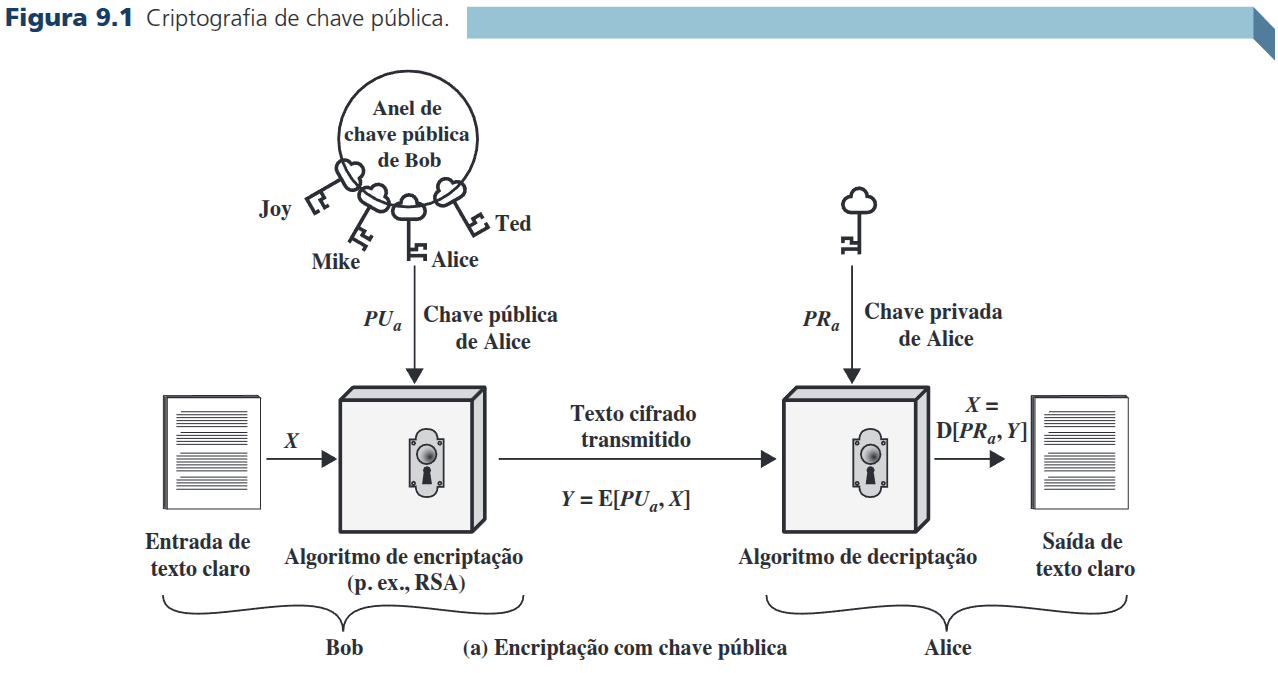
\includegraphics[width=\linewidth]{Figuras/encriptacao-com-chave-publica.png}

  \end{figure}

\end{frame}

\begin{frame}{Encriptação com chave privada}

  \begin{figure}
    \centering
    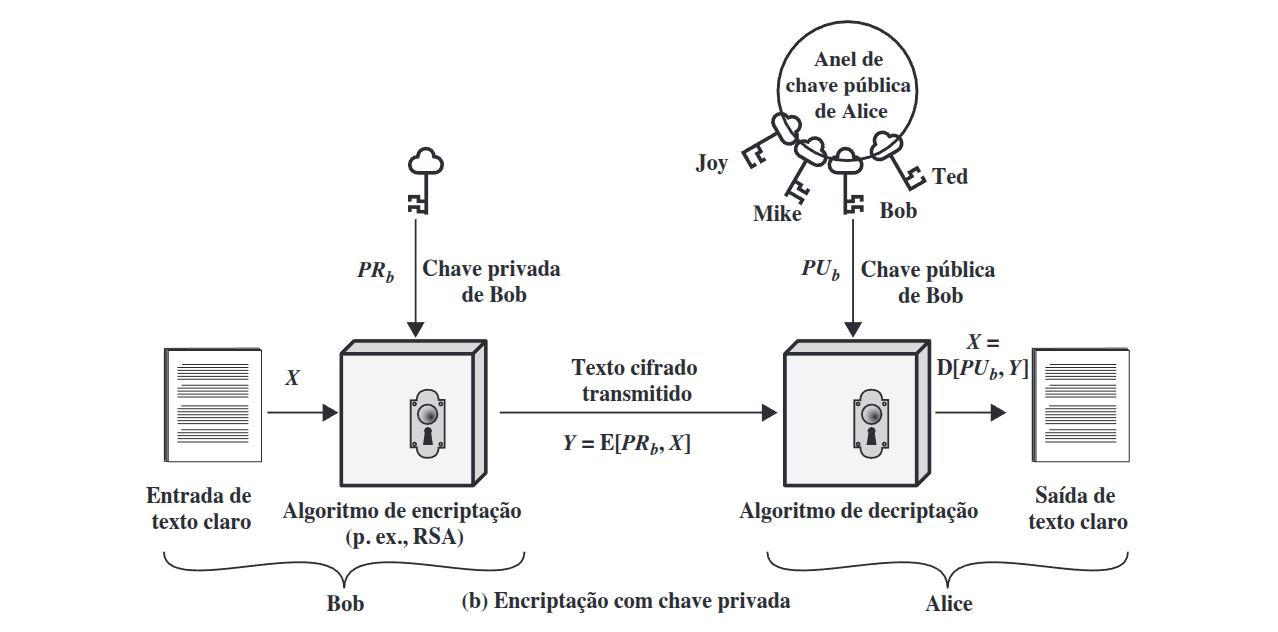
\includegraphics[width=\linewidth]{Figuras/encriptacao-com-chave-privada.png}

  \end{figure}

\end{frame}

\begin{frame}{Etapas Essenciais da Criptografia de Chave Pública}
  \begin{enumerate}
    \item Cada usuário gera um \textbf{par de chaves} (pública e privada) para encriptação e decriptação.
    \item A \textbf{chave pública} é disponibilizada em um repositório ou arquivo acessível; a \textbf{chave privada} permanece secreta.
    \item Para enviar uma mensagem confidencial a Alice, Bob usa a \textbf{chave pública de Alice} para encriptar a mensagem.
    \item Ao receber, Alice utiliza sua \textbf{chave privada} para decriptar. Apenas ela consegue recuperar o texto original.
  \end{enumerate}
\end{frame}


\begin{frame}{Esquema de Encriptação de Chave Pública}
  Um esquema de encriptação de chave pública possui cinco elementos principais:
  \begin{enumerate}
    \item \textbf{Texto claro}: mensagem ou dados legíveis fornecidos como entrada.
    \item \textbf{Algoritmo de encriptação}: aplica transformações no texto claro.
    \item \textbf{Chaves pública e privada}: par de chaves; se uma encripta, a outra decripta.
    \item \textbf{Texto cifrado}: mensagem embaralhada gerada como saída, dependente da chave.
    \item \textbf{Algoritmo de decriptação}: reverte o processo, recuperando o texto claro original.
  \end{enumerate}
\end{frame}

\begin{frame}{Criptossitema de chave pública - Objetivo Sigilo}

  \begin{figure}
    \centering
    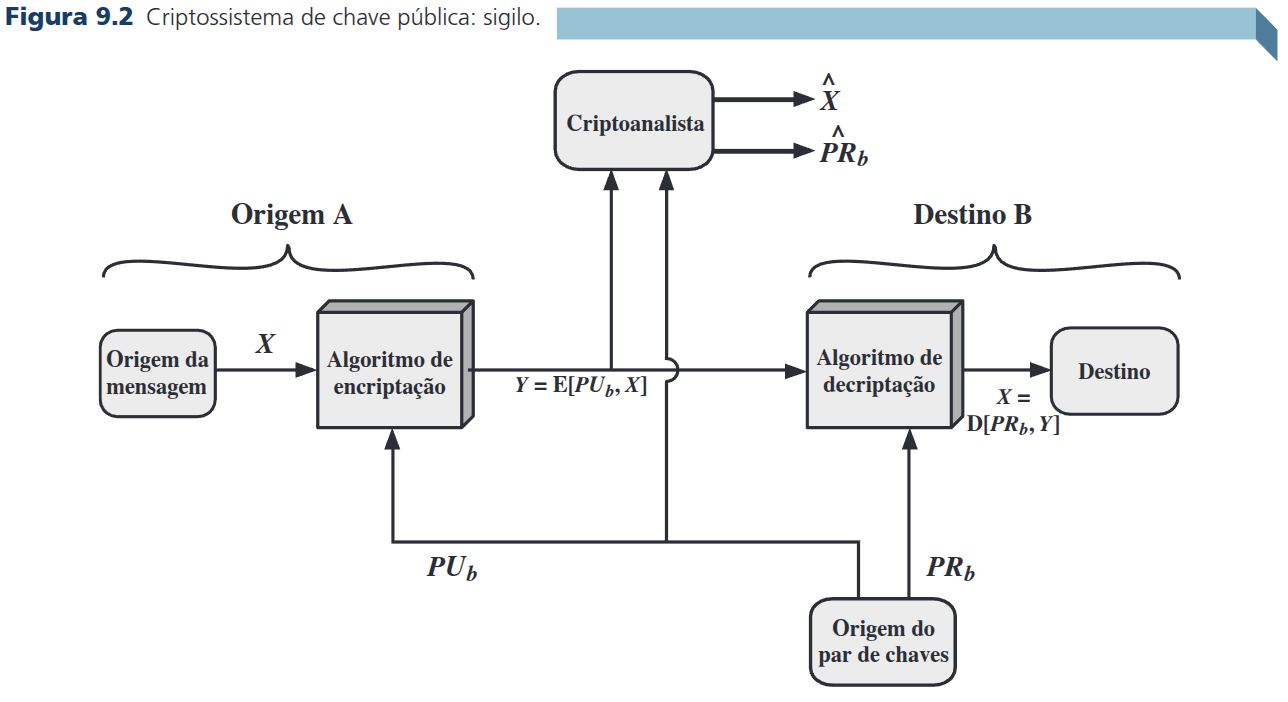
\includegraphics[width=\linewidth]{Figuras/criptossistema-chave-publica.png}

  \end{figure}

\end{frame}

\begin{frame}{Criptossitema de chave pública - Objetivo autenticação}

  \begin{figure}
    \centering
    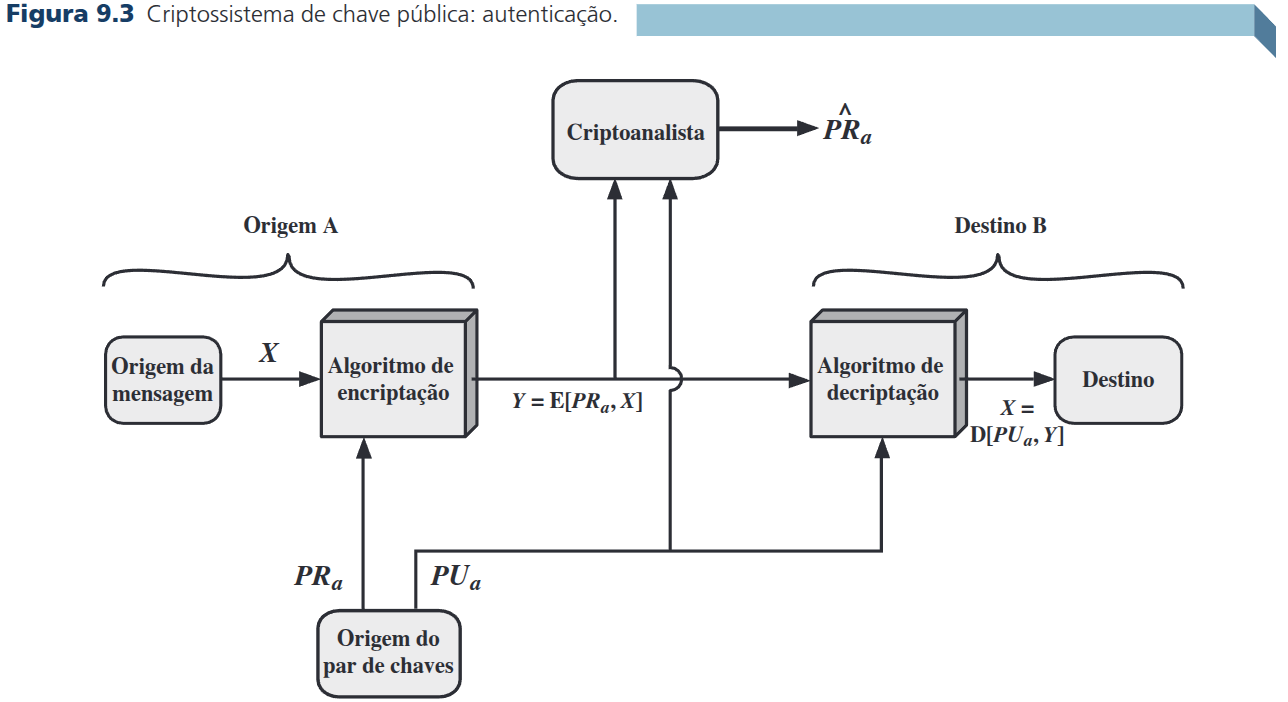
\includegraphics[width=0.9\linewidth]{Figuras/criptossistema-chave-publica-autenticacao.png}

  \end{figure}

\end{frame}

\begin{frame}{Autenticação e Confidencialidade com Chave Pública}
  \textbf{Importante}:
  \begin{itemize}
    \item Apenas a encriptação com a chave privada do emissor garante \textbf{autenticação}, mas não a confidencialidade.
    \item Para prover \textbf{ambos}, aplica-se uma dupla encriptação:
  \end{itemize}

  \[
    Z = E(PU_b, \; E(PR_a, \; X))
  \]
  \[
    X = D(PU_a, \; D(PR_b, \; Z))
  \]

  \begin{itemize}
    \item O emissor primeiro encripta com sua \textbf{chave privada} (assinatura digital).
    \item Em seguida, encripta novamente com a \textbf{chave pública do receptor}.
    \item O receptor, ao decriptar, recupera tanto a \textbf{confidencialidade} quanto a \textbf{autenticidade}.
    \item Desvantagem: exige 4 operações de criptografia assimétrica por mensagem.
  \end{itemize}
\end{frame}

\begin{frame}{Criptossitema de chave pública - Objetivo autenticação e sigilo}

  \begin{figure}
    \centering
    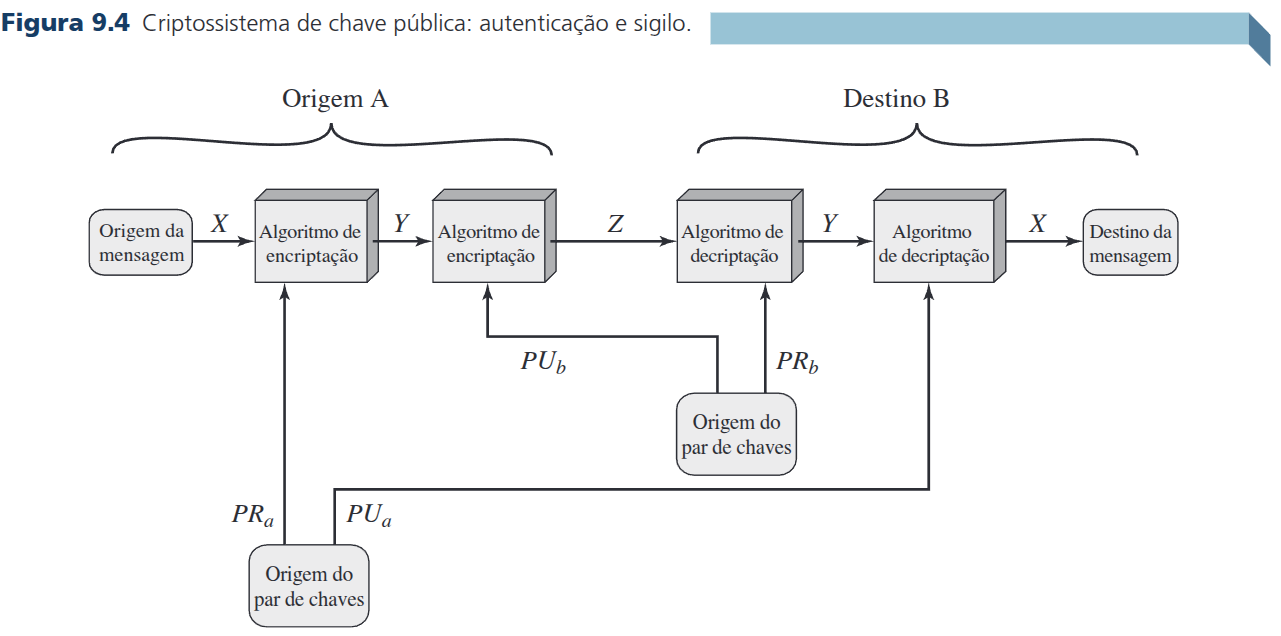
\includegraphics[width=\linewidth]{Figuras/criptossistema-de-chave-publica-autenticacao-e-sigilo.png}

  \end{figure}

\end{frame}

\begin{frame}{Aplicações de criptografia de chave pública}

  \begin{figure}
    \centering
    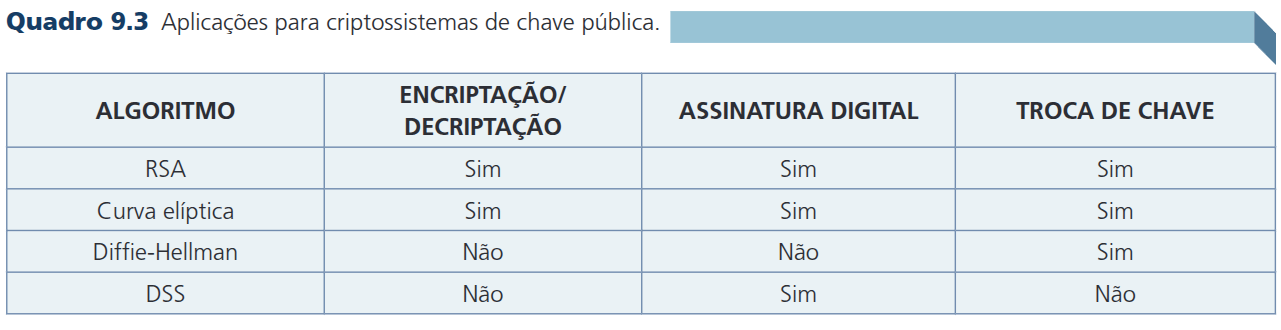
\includegraphics[width=\linewidth]{Figuras/aplicacoes-criptografia-chave-publica.png}

  \end{figure}
  \textbf{Obs}: DSS é a sigla para
  Digital Signature Standard, um padrão de assinatura digital que, em conjunto com o DSA (Digital Signature Algorithm) e o SHA (Secure Hash Algorithm), permite a criação de assinaturas digitais e verificação de integridade de dados, utilizando criptografia de chave pública de forma a garantir a autenticidade e a não-repudiação de uma transação
\end{frame}

\begin{frame}{Requisitos para Criptografia de Chave Pública}
  \begin{enumerate}
    \item Geração de par de chaves $(PU_b, PR_b)$ deve ser \textbf{computacionalmente fácil}.
    \item Encriptação: dado $PU_b$ e $M$, calcular $C = E(PU_b, M)$ deve ser \textbf{fácil}.
    \item Decriptação: dado $PR_b$ e $C$, calcular $M = D(PR_b, C)$ deve ser \textbf{fácil}.
    \item \textbf{Inviável} obter $PR_b$ a partir de $PU_b$.
    \item \textbf{Inviável} recuperar $M$ conhecendo apenas $PU_b$ e $C$.
    \item (Opcional) Ordem das chaves pode ser invertida:
          $M = D[PU_b, E(PR_b, M)] = D[PR_b, E(PU_b, M)]$.
  \end{enumerate}

  \vspace{0.3cm}
  \textbf{Observação:} Apenas poucos algoritmos atendem a todos os requisitos, como RSA, ECC, Diffie-Hellman e DSS.
\end{frame}
\begin{frame}{Função de Mão Única com Alçapão}
  \begin{itemize}
    \item Função de mão única: mapeia um domínio $X$ em um intervalo $Y$ de forma que:
          \[
            Y = f(X) \text{ é fácil de calcular, mas } X = f^{-1}(Y) \text{ é inviável de obter.}
          \]
    \item "Com alçapão": existe uma informação secreta que permite inverter a função de forma eficiente.
    \item Essencial para criptografia de chave pública: permite encriptação segura sem compartilhar a chave privada.
  \end{itemize}

\end{frame}

\begin{frame}{Complexidade de Funções Criptográficas}
  \begin{itemize}
    \item \textbf{Fácil}: problema resolvível em tempo polinomial $O(n^a)$ em função do tamanho da entrada $n$. Onde $a$ é uma constante fixa.
    \item Algoritmos polinomiais pertencem à classe P.
    \item \textbf{Inviável}: problema cujo esforço cresce mais rápido que o tempo polinomial, por exemplo, $O(2^n)$.
    \item Observação: medir complexidade pelo pior caso ou caso médio não é suficiente para criptografia.
    \item Criptografia exige que a função seja inviável de reverter para \textbf{praticamente todas as entradas}.
  \end{itemize}
\end{frame}
\begin{frame}{Função de Mão Única com Alçapão}
  \begin{itemize}
    \item Uma função que é fácil de calcular em uma direção e inviável na outra, a menos que informação adicional (alçapão) seja conhecida.
    \item Formalmente, uma família de funções reversíveis $f_k$:
          \begin{itemize}
            \item $Y = f_k(X)$ é fácil, se $k$ e $X$ forem conhecidos.
            \item $X = f_k^{-1}(Y)$ é fácil, se $k$ e $Y$ forem conhecidos.
            \item $X = f_k^{-1}(Y)$ é inviável, se apenas $Y$ for conhecido, sem $k$.
          \end{itemize}
    \item A construção de esquemas de \textbf{chave pública} depende de \textbf{encontrar funções de mão única com alçapão adequadas}.
  \end{itemize}
\end{frame}

\begin{frame}{Algoritmo RSA}
  \begin{itemize}
    \item O artigo de Diffie e Hellman (1976) desafiou a comunidade a criar algoritmos de chave pública. \href{https://dl.acm.org/doi/10.1145/1499799.1499815}{\textcolor{blue}{Referência}}
    \item Muitos algoritmos iniciais se mostraram falhos.
    \item Em 1977, Ron Rivest, Adi Shamir e Len Adleman (MIT) desenvolveram o esquema RSA. \href{https://dl.acm.org/doi/10.1145/359340.359342}{\textcolor{blue}{Referência}}
    \item Publicado em 1978, o RSA se tornou a técnica mais aceita e amplamente implementada para criptografia de chave pública.
  \end{itemize}
\end{frame}
\begin{frame}{Funcionamento do RSA}
  \begin{itemize}
    \item RSA é uma cifra de bloco: texto claro e cifrado são inteiros entre 0 e $n-1$.
    \item Tamanho típico: $n \approx 1024$ bits (309 dígitos decimais).
    \item Cada bloco de texto claro $M$ deve satisfazer $0 \le M < n$.
    \item Encriptação e decriptação:
          \[
            C = M^e \mod n,
          \]
          \[
            \quad M = C^d \mod n = (M^e)^d \mod n
          \]
    \item Chave pública: $PU = \{e, n\}$
          Chave privada: $PR = \{d, n\}$
    \item Requisitos:
          \begin{enumerate}
            \item $M^{ed} \mod n = M$ para todo $M < n$
            \item Calcular $M^e \mod n$ e $C^d \mod n$ é relativamente fácil
            \item Conhecendo $e$ e $n$, é inviável determinar $d$
          \end{enumerate}
    \item $d$ pode ser calculado usando o algoritmo de Euclides estendido
  \end{itemize}
\end{frame}
\begin{frame}{Requisito de Inversão no RSA}
  \begin{itemize}
    \item Para garantir $M^{ed} \mod n = M$, os expoentes $e$ e $d$ devem ser inversos multiplicativos módulo $\varphi(n)$, onde $\varphi(n)$ é a função totiente de Euler.
    \item Para $n = pq$, com $p$ e $q$ primos:
          \[
            \varphi(n) = (p-1)(q-1)
          \]
    \item Relação entre $e$ e $d$:
          \[
            ed \equiv 1 \mod \varphi(n) \quad \Rightarrow \quad d \equiv e^{-1} \mod \varphi(n)
          \]
    \item Condição: $e$ e $d$ devem ser relativamente primos a $\varphi(n)$:
          \[
            \gcd(d, \varphi(n)) = 1
          \]
  \end{itemize}

\end{frame}

\begin{frame}{Inverso Multiplicativo no RSA}
  No RSA, a chave privada $d$ é escolhida como o inverso multiplicativo de $e$ módulo $\varphi(n)$:

  \[
    d \equiv e^{-1} \pmod{\varphi(n)}
  \]

  \begin{itemize}
    \item Isso significa que $d$ satisfaz:
          \[
            d \cdot e \equiv 1 \pmod{\varphi(n)}
          \]
    \item Exemplo: $e = 7$, $\varphi(n) = 160$
          \[
            23 \cdot 7 = 161 \equiv 1 \pmod{160}
          \]
    \item Portanto, $d = 23$ é o inverso multiplicativo de $e = 7$ módulo 160.

  \end{itemize}
\end{frame}


\begin{frame}{Esquema RSA}
  \textbf{Ingredientes:}
  \begin{itemize}
    \item Dois números primos secretos: $p$ e $q$.
    \item Calcula-se $n = pq$ (público).
    \item Escolhe-se $e$ tal que $mdc(\varphi(n), e) = 1$ e $1 < e < \varphi(n)$ (público).
    \item Calcula-se $d \equiv e^{-1} \mod \varphi(n)$ (privado).
  \end{itemize}

  \textbf{Chaves:}
  \begin{itemize}
    \item Chave privada: $\{d, n\}$
    \item Chave pública: $\{e, n\}$
  \end{itemize}

  \textbf{Processo de encriptação e decriptação:}
  \begin{itemize}
    \item Usuário B quer enviar mensagem $M$ para A:
          \[
            C = M^e \mod n \quad \text{(encriptação)}
          \]
    \item Usuário A recebe $C$ e decripta:
          \[
            M = C^d \mod n
          \]
  \end{itemize}
\end{frame}
\begin{frame}{Tabela resumo dos parâmetros do RSA}

  \begin{figure}
    \centering
    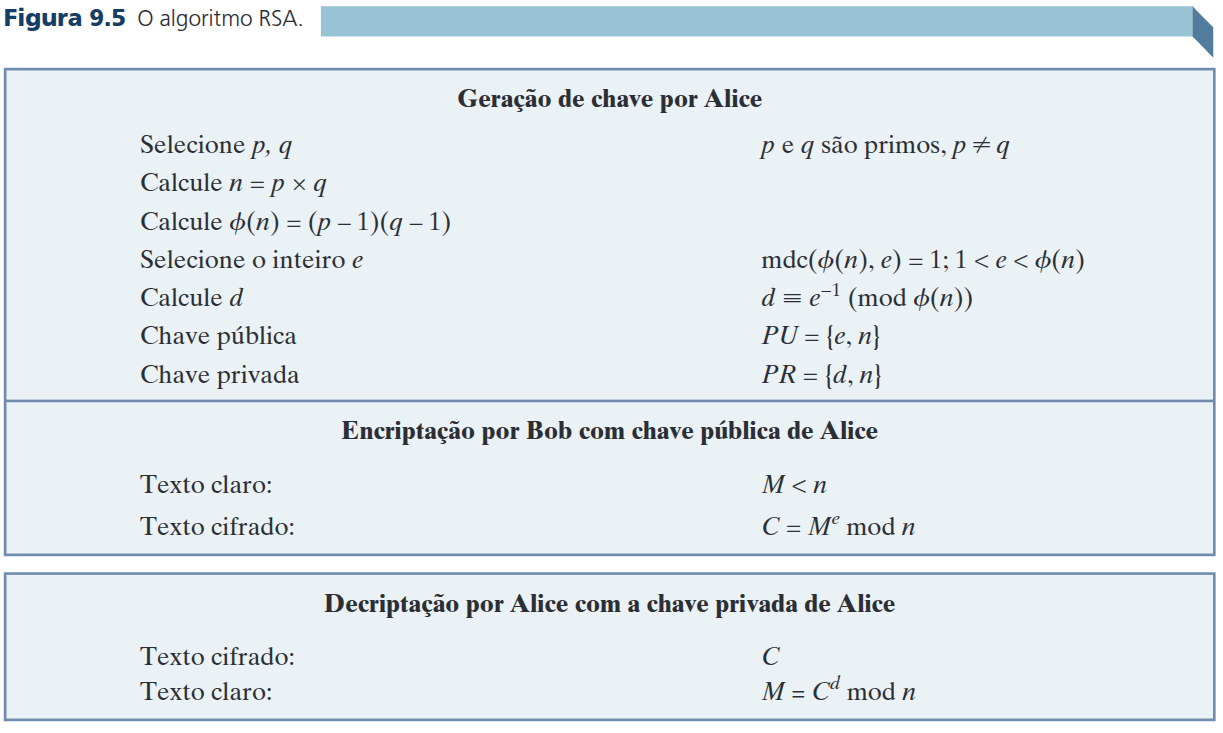
\includegraphics[width=0.8\linewidth]{Figuras/tabela-resumo-rsa.png}

  \end{figure}

\end{frame}
\begin{frame}{Exemplo Numérico do RSA}
  \textbf{Geração de chaves:}
  \begin{itemize}
    \item $p = 17$, $q = 11$
    \item $n = pq = 187$
    \item $\varphi(n) = (p-1)(q-1) = 160$
    \item Escolhe $e = 7$, $mdc(e, 160) = 1$
    \item Calcula $d \equiv e^{-1} \mod 160 \Rightarrow d = 23$
  \end{itemize}

  \begin{block}{Explicação}
    \begin{itemize}
      \item Exemplo: $e = 7$, $\varphi(n) = 160$
            \[
              23 \cdot 7 = 161 \equiv 1 \pmod{160}
            \]
      \item Portanto, $d = 23$ é o inverso multiplicativo de $e = 7$ módulo 160.

    \end{itemize}

  \end{block}

  \textbf{Chaves:}
  \begin{itemize}
    \item Pública: $PU = \{7, 187\}$
    \item Privada: $PR = \{23, 187\}$
  \end{itemize}
\end{frame}
\begin{frame}{Exemplo Numérico do RSA}
  \textbf{Encriptação de $M = 88$:}
  \[
    C = M^e \mod n = 88^7 \mod 187
  \]
  \[
    88^7 \mod 187 = (88 \times 88^2 \times 88^4) \mod 187 = (88 \times 77 \times 132) \mod 187 = 11
  \]

  \textbf{Decriptação:}
  \[
    M = C^d \mod n = 11^{23} \mod 187
  \]
  \[
    11^{23} \mod 187 = 88
  \]

  \textbf{Resultado:} A mensagem original $M = 88$ é recuperada com sucesso.
\end{frame}
\begin{frame}{Exemplo Simples numérico - RSA}

  \begin{figure}
    \centering
    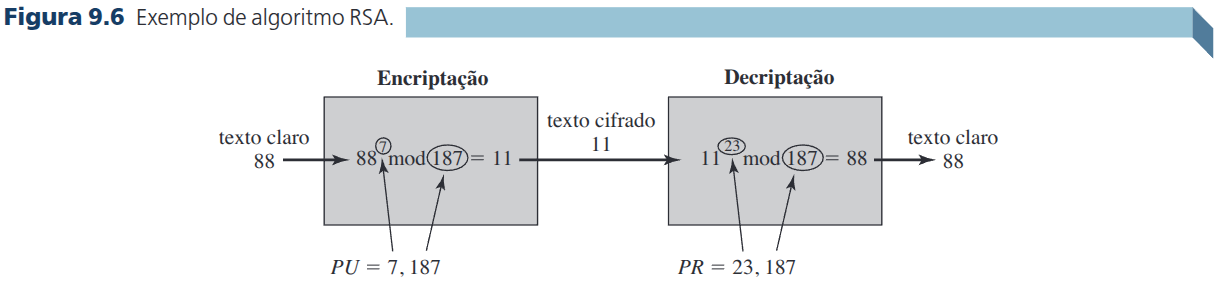
\includegraphics[width=\linewidth]{Figuras/exemplo-rsa-numerico-simples.png}

  \end{figure}

\end{frame}

\begin{frame}{Processamento de múltiplos blocos usando RSA}

  \begin{figure}
    \centering
    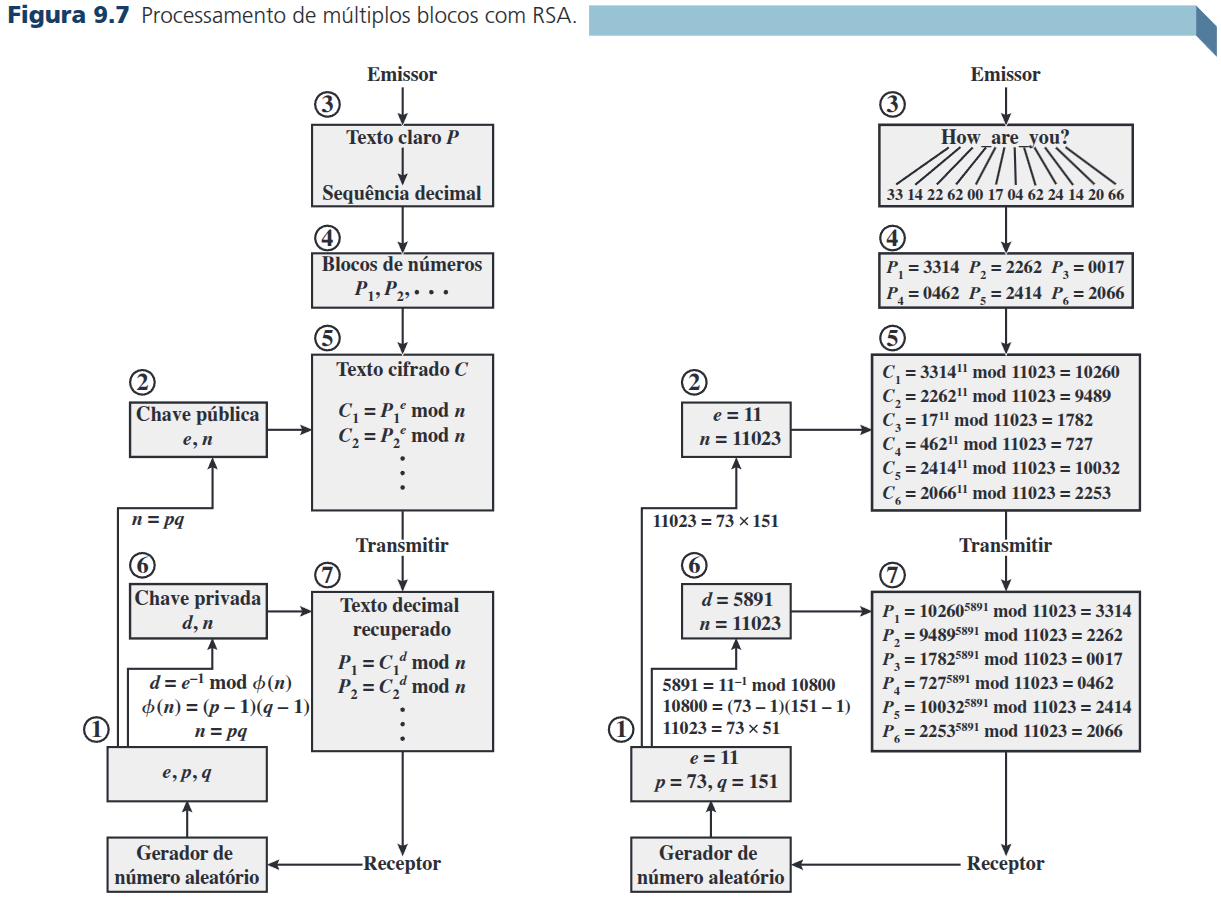
\includegraphics[width=0.7\linewidth]{Figuras/processamento-multiplos-blocos-rsa.png}

  \end{figure}

\end{frame}
%\title{Aula 12 - IPsec}

\author{Prof. Gabriel Rodrigues Caldas de Aquino}

\institute
{
    Instituto de Computação \\
    Universidade Federal do Rio de Janeiro\\
    gabrielaquino@ic.ufrj.br% Your institution for the title page
}
\date{Compilado em: \\ \today} % Date, can be changed to a custom date

%----------------------------------------------------------------------------------------
%    PRESENTATION SLIDE
%----------------------------------------------------------------------------------------



\begin{frame}
    % Print the title page as the first slide
    \titlepage
\end{frame}

\begin{frame}{IPsec: O Protocolo IP de Segurança}
    \begin{itemize}
        \item Provê segurança na camada de rede.
        \item Protege datagramas IP entre quaisquer entidades (dispositivos finais (\textit{hosts}), roteadores).
        \item Usado para criar Redes Privadas Virtuais (VPNs) sobre a Internet pública.
        \item Definido pelo IAB como essencial para o IPv6 (autenticação e criptografia).
        \item Projetado para ser compatível tanto com IPv4 quanto com IPv6.
        \item Atualmente, muitos fabricantes já oferecem suporte ao IPsec.
    \end{itemize}
\end{frame}

\begin{frame}{Relembrando encapsulamento em redes}


    \begin{figure}
        \centering
        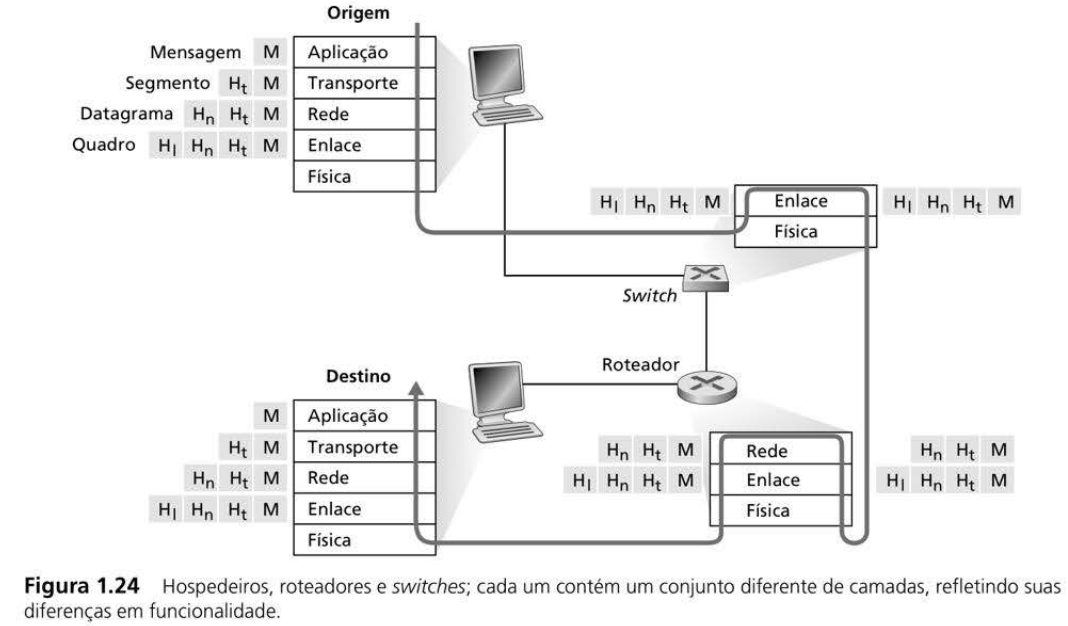
\includegraphics[width=0.7\textwidth]{Figuras/encapsulamento-pilha-protocolos.png}
    \end{figure}



\end{frame}

\begin{frame}{Relembrando o formato do datagrama IPv4}


    \begin{figure}
        \centering
        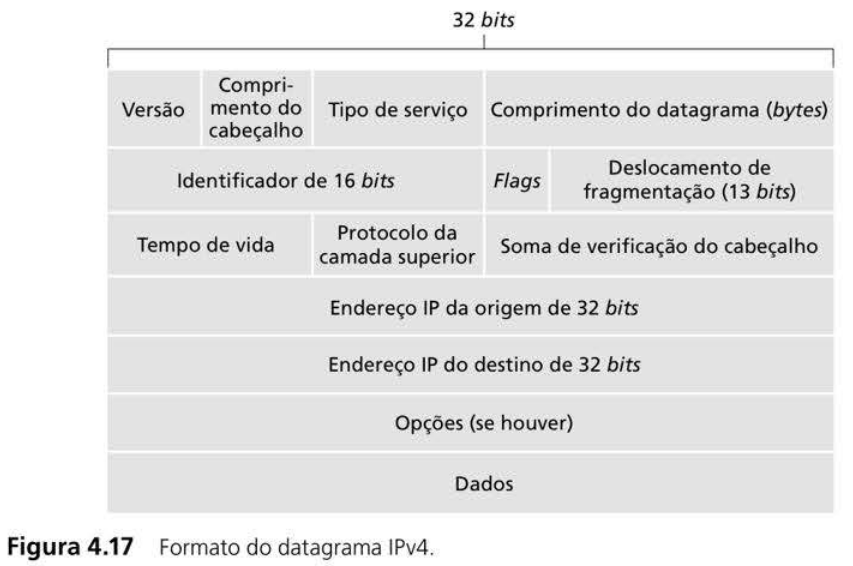
\includegraphics[width=0.7\textwidth]{Figuras/formato-datagrama-ipv4.png}
    \end{figure}



\end{frame}

\begin{frame}{Áreas Funcionais da Segurança em Nível IP}
    \begin{itemize}
        \item A segurança em nível IP abrange três áreas funcionais:
    \end{itemize}

    \begin{block}{1. Autenticação}
        \begin{itemize}
            \item Garante que o pacote foi realmente enviado pela fonte identificada.
            \item Assegura que o pacote não foi alterado durante o trânsito.
        \end{itemize}
    \end{block}

    \begin{block}{2. Confidencialidade}
        \begin{itemize}
            \item Permite aos nós da rede cifrar (criptografar) mensagens.
            \item Previne a espionagem (eavesdropping) por terceiros.
        \end{itemize}
    \end{block}

    \begin{block}{3. Gerenciamento de Chaves}
        \begin{itemize}
            \item Trata da troca segura de chaves entre as partes.
        \end{itemize}
    \end{block}
\end{frame}

\begin{frame}{O Conceito de Sigilo na Camada de Rede}
    \begin{itemize}
        \item O que significa prover sigilo na camada de rede?
              \begin{itemize}
                  \item A entidade remetente (hospedeiro ou roteador) cifra as \textbf{cargas úteis (payloads)} de todos os datagramas que envia.
              \end{itemize}

        \item O que é a carga útil (payload)?
              \begin{itemize}
                  \item Segmento TCP
                  \item Segmento UDP
                  \item Mensagem ICMP
                  \item Mensagem SNMP, etc.
              \end{itemize}

        \item Resultado: \textbf{"Cobertura Total" }
              \begin{itemize}
                  \item Todos os dados (e-mails, páginas Web, mensagens de gerenciamento) ficam ocultos de intrusos.
              \end{itemize}
    \end{itemize}
\end{frame}



\begin{frame}{Outros Serviços de Segurança da Camada de Rede}
    Além da confidencialidade, um protocolo de segurança da camada de rede pode prover:
    \begin{itemize}

        \item \textbf{Autenticação da Origem}
              \begin{itemize}
                  \item Permite à entidade destinatária verificar a origem (remetente) do datagrama protegido.
              \end{itemize}

        \item \textbf{Integridade dos Dados}
              \begin{itemize}
                  \item Permite à entidade destinatária verificar se o datagrama sofreu qualquer adulteração durante o trânsito.
              \end{itemize}

        \item \textbf{Prevenção do Ataque de Repetição (Replay Attack)}
              \begin{itemize}
                  \item Permite ao destinatário (Bob) detectar quaisquer datagramas duplicados que um atacante possa inserir no fluxo.
              \end{itemize}
        \item \textbf{Característica:} IPsec pode \textbf{criptografar e/ou autenticar todo o tráfego no nível IP}.
    \end{itemize}


\end{frame}
\begin{frame}{Aplicações Comuns do IPsec}

    \begin{itemize}
        \item O IPsec pode ser usado em LANs, WANs (públicas/privadas) e na Internet.
        \item Todas as aplicações distribuídas se beneficiam, sem necessidade de modificação.

        \item \textbf{Exemplos de uso:}
              \begin{itemize}
                  \item \textbf{Conectividade Segura de Filiais (VPN):}
                        \begin{itemize}
                            \item Permite construir uma VPN segura sobre a Internet.
                            \item Reduz custos e a necessidade de redes privadas.
                        \end{itemize}

                  \item \textbf{Acesso Remoto Seguro:}
                        \begin{itemize}
                            \item Usuários remotos (viajantes, telecommuters) acessam a rede da empresa de forma segura através de um ISP local.
                        \end{itemize}

                  \item \textbf{Conectividade Extranet/Intranet com Parceiros:}
                        \begin{itemize}
                            \item Protege a comunicação com outras organizações (autenticação, confidencialidade, troca de chaves).
                        \end{itemize}

                  \item \textbf{Reforço à Segurança de E-commerce:}
                        \begin{itemize}
                            \item Adiciona segurança, mesmo que as aplicações Web já possuam protocolos de segurança próprios.
                        \end{itemize}
              \end{itemize}
    \end{itemize}
\end{frame}

\begin{frame}{Benefícios do IPsec}
    \begin{itemize}
        \item \textbf{Implementação em Firewall/Roteador}
              \begin{itemize}
                  \item Aplica segurança forte a todo o tráfego que cruza o perímetro.
                  \item O tráfego interno (workgroup) não sofre overhead de processamento.
              \end{itemize}

        \item \textbf{Resistência a Bypass}
              \begin{itemize}
                  \item Difícil de contornar (bypass) se o firewall IPsec for a única entrada da Internet.
              \end{itemize}

        \item \textbf{Transparência para Aplicações}
              \begin{itemize}
                  \item Atua abaixo da camada de transporte (TCP/UDP).
                  \item Não exige mudança de software em usuários ou servidores.
                  \item Aplicações de camada superior não são afetadas.
              \end{itemize}
        \item \textbf{Transparência para o Usuário Final}
              \begin{itemize}
                  \item Não é necessário treinar os usuários sobre os mecanismos de segurança.
                  \item Não é preciso gerenciar chaves por usuário (emitir/revogar).
              \end{itemize}

        \item \textbf{Flexibilidade (Segurança Individual)}
              \begin{itemize}
                  \item Pode prover segurança para usuários individuais, se necessário.
                  \item Útil para trabalhadores remotos (off-site).
                  \item Permite criar sub-redes virtuais seguras para aplicações sensíveis.
              \end{itemize}
    \end{itemize}
\end{frame}

\begin{frame}{IPsec e Redes Privadas Virtuais (VPNs)}
    \begin{itemize}
        \item \textbf{O Cenário:}
              \begin{itemize}
                  \item Instituições que se estendem por diversas regiões geográficas.
              \end{itemize}

        \item \textbf{A Necessidade:}
              \begin{itemize}
                  \item Desejam ter sua própria rede IP.
                  \item Objetivo: Permitir que seus hospedeiros e servidores enviem dados uns aos outros de forma segura e sigilosa.
              \end{itemize}

        \item \textbf{A Solução Tradicional: Rede Privada}
              \begin{itemize}
                  \item Definição: Uma rede física independente, reservada a uma instituição particular.
                  \item Características:
                  \item É completamente separada da Internet pública.
                  \item Requer infraestrutura própria: roteadores, enlaces e DNS.
              \end{itemize}

        \item \textbf{O Problema da Rede Privada:}
              \begin{itemize}
                  \item Custo muito elevado.
                  \item A instituição precisa comprar, instalar e manter sua própria infraestrutura de rede física.
              \end{itemize}
    \end{itemize}
\end{frame}

\begin{frame}{A Solução: Rede Privada Virtual (VPN)}
    \begin{itemize}
        \item  VPNs operam "em cima" (sobre) da Internet pública.
        \item O tráfego é  \textbf{criptografado} e enviado através da infraestrutura da Internet pública.
        \item Não é necessária uma rede fisicamente independente e dedicada.

        \item A criptografia é aplicada \textbf{antes} que os pacotes entrem na Internet pública.
    \end{itemize}


    % Você pode inserir sua figura aqui
    \begin{figure}
        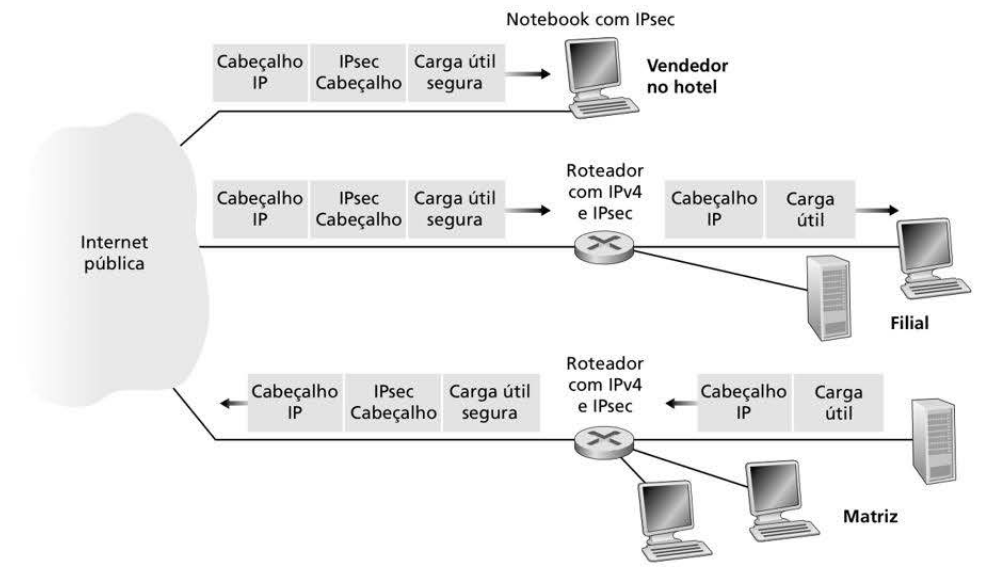
\includegraphics[width=0.68\textwidth]{Figuras/ipsec-vpn.png}
        \label{fig:vpn}
    \end{figure}
\end{frame}

\begin{frame}{VPN: Cenário de Exemplo e Fluxo de Tráfego}
    \begin{itemize}
        \item \textbf{Componentes da Instituição (Exemplo):}
              \begin{itemize}
                  \item Matriz, Filial e outros acessando da Internet

              \end{itemize}

        \item \textbf{Fluxo 1: Comunicação Interna (Dentro de um Local)}
              \begin{itemize}
                  \item Ex: Hospedeiro na Matriz $\leftrightarrow$ Hospedeiro na Matriz.
                  \item Ex: Hospedeiro na Filial $\leftrightarrow$ Hospedeiro na Filial.
                  \item Método: IP v4 padrão (sem IPsec). O tráfego não sai para a rede pública.
              \end{itemize}

        \item \textbf{Fluxo 2: Comunicação Externa (Entre Locais via VPN)}
              \begin{itemize}
                  \item Ex: Hospedeiro na Matriz $\leftrightarrow$ Hospedeiro na Filial.
                  \item Ex: Vendedor Viajante $\leftrightarrow$ Hospedeiro na Matriz.
                  \item Caminho: O tráfego deve cruzar a Internet pública.
                  \item Método: O tráfego é \textbf{codificado (criptografado)} antes de entrar na Internet (usando IPsec).
              \end{itemize}
    \end{itemize}
\end{frame}

\begin{frame}{Tráfego Misto: IPsec e IPv4 Comum}
    \begin{itemize}
        \item \textbf{Ponto Importante:}
              \begin{itemize}
                  \item Nem todo o tráfego enviado à Internet pelos roteadores de borda ou pelos notebooks será protegido por IPsec.
              \end{itemize}

        \item \textbf{Exemplo: Acesso à Internet Pública}
              \begin{itemize}
                  \item Um hospedeiro na matriz quer acessar um servidor Web comum (ex: Amazon, Google).
                  \item Este tráfego não é destinado à VPN.
              \end{itemize}

        \item \textbf{Resultado: Coexistência de Tráfego}
              \begin{itemize}
                  \item O roteador de borda (e os notebooks) emitirão \textbf{ambos} os tipos de datagramas para a Internet:
                        \begin{itemize}
                            \item Datagramas IPv4 comuns (para tráfego público).
                            \item Datagramas IPsec seguros (para tráfego da VPN).
                        \end{itemize}
              \end{itemize}
    \end{itemize}
\end{frame}

\begin{frame}{VPN: Fluxo de Tráfego (Matriz $\rightarrow$ Vendedor Viajante)}
    \begin{itemize}
        \item \textbf{1. Na Matriz (Origem)}
              \begin{itemize}
                  \item Um hospedeiro envia um datagrama IPv4 padrão (ex: TCP/UDP).
              \end{itemize}

        \item \textbf{2. No Roteador de Borda (Gateway IPsec da Matriz)}
              \begin{itemize}
                  \item Intercepta o datagrama IPv4.
                  \item Converte o datagrama IPv4 em um datagrama \textbf{IPsec}.
                  \item Encaminha o pacote IPsec para a Internet.
              \end{itemize}

        \item \textbf{3. Na Internet (Trânsito)}
              \begin{itemize}
                  \item O datagrama IPsec possui um cabeçalho IPv4 tradicional (externo).
                  \item Roteadores da Internet o processam como um datagrama IPv4 comum.
              \end{itemize}

        \item \textbf{4. Estrutura do Pacote IPsec (no Trânsito)}
              \begin{itemize}
                  \item A carga útil (payload) do datagrama IPsec contém:
                        \begin{itemize}
                            \item Um \textbf{cabeçalho IPsec} (para processamento de segurança).
                            \item A carga útil original (ex: segmento TCP/UDP), que está \textbf{codificada} (criptografada).
                        \end{itemize}
              \end{itemize}

        \item \textbf{5. No Notebook do Vendedor (Destino)}
              \begin{itemize}
                  \item O S.O. recebe o datagrama IPsec.
                  \item \textbf{Decodifica} a carga útil (descriptografa).
                  \item Verifica outros serviços (ex: integridade dos dados).
                  \item Passa a carga útil original (não codificada) para a camada superior (TCP ou UDP).
              \end{itemize}
    \end{itemize}
\end{frame}

\begin{frame}{Protocolos Principais do IPsec: AH vs. ESP}
    O conjunto IPsec possui dois protocolos principais para envio de dados seguros (entre hospedeiros ou roteadores):
    \begin{itemize}


        \item \textbf{1. Protocolo Cabeçalho de Autenticação (AH - Authentication Header)}
              \begin{itemize}


                  \item \textbf{Provê} Autenticação da Origem.
                  \item \textbf{Provê} Integridade dos Dados.

                  \item \textbf{NÃO} provê Sigilo (Confidencialidade).
              \end{itemize}

        \item \textbf{2. Protocolo Carga de Segurança de Encapsulamento (ESP - Encapsulating Security Payload)}
              \begin{itemize}


                  \item \textbf{Provê} Autenticação da Origem.
                  \item \textbf{Provê} Integridade dos Dados.
                  \item \textbf{Provê} \textbf{Sigilo (Confidencialidade)} $\leftarrow$ (Função combinada de autenticação/criptografia).

              \end{itemize}
    \end{itemize}
\end{frame}

\begin{frame}{O Foco no ESP (AH é Deprecated)}
    \begin{itemize}
        \item \textbf{Por que o ESP é muito mais utilizado?}
              \begin{itemize}
                  \item O Sigilo (Criptografia) é muitas vezes essencial para VPNs.
                  \item VPNs geralmente desejam \textbf{autenticação E criptografia} para:
                        \begin{itemize}
                            \item 1. Impedir que usuários não autorizados penetrem na rede.
                            \item 2. Impedir que espiões (eavesdroppers) na Internet leiam as mensagens.
                        \end{itemize}
              \end{itemize}

        \item \textbf{O Status Atual do AH}: é \textbf{deprecated} (obsoleto)
              \begin{itemize}

                  \item Motivo: O próprio protocolo ESP já fornece a autenticação da mensagem.
                  \item O AH é mantido no IPsecv3 apenas para \textit{backward compatibility} (compatibilidade retroativa).
                  \item \textbf{Não deve ser usado em novas aplicações.}
              \end{itemize}

        \item \textbf{Foco atual:} \textbf{ESP}.

    \end{itemize}
\end{frame}

\begin{frame}{Associações de Segurança (SA)}
    \begin{itemize}
        \item Datagramas IPsec são enviados entre pares de entidades da rede (hospedeiro $\leftrightarrow$ hospedeiro, roteador $\leftrightarrow$ roteador, etc.).

        \item \textbf{O que é uma Associação de Segurança (SA - \textit{Security Association})?}
              \begin{itemize}

                  \item É uma \textbf{conexão lógica} da camada de rede.
                  \item Criada \textbf{antes} que a entidade remetente possa enviar datagramas IPsec à entidade destinatária.
              \end{itemize}

        \item \textbf{Característica Chave: Unidirecional}
              \begin{itemize}
                  \item Uma SA é uma conexão lógica \textbf{simples} (simplex).
                  \item Ela flui em apenas uma direção: do remetente para o destinatário.
              \end{itemize}

        \item \textbf{Comunicação Bidirecional (Mútua)}
              \begin{itemize}
                  \item Se duas entidades querem enviar dados seguros entre si (nos dois sentidos): Precisam ser estabelecidas \textbf{duas SAs} (duas conexões lógicas).
                  \item Uma SA em cada direção.
              \end{itemize}
    \end{itemize}
\end{frame}

\begin{frame}{Exemplo: Contagem de SAs em uma VPN}
    \begin{itemize}
        \item \textbf{Cenário (Instituição):}
              \begin{itemize}
                  \item 1 Matriz.
                  \item 1 Filial.
                  \item $n$ Vendedores Viajantes (notebooks).
              \end{itemize}

        \item \textbf{Fluxos de Tráfego IPsec (Bidirecional):}
              \begin{itemize}
                  \item Tráfego bidirecional entre o roteador de borda da Matriz e o roteador de borda da Filial.
                  \item Tráfego bidirecional entre o roteador de borda da Matriz e CADA UM dos $n$ Vendedores.
              \end{itemize}

        \item \textbf{Cálculo - Quantidade de SA:}
              \begin{itemize}
                  \item \textbf{Matriz $\leftrightarrow$ Filial:}
                        \begin{itemize}
                            \item 1 SA (Matriz $\rightarrow$ Filial)
                            \item 1 SA (Filial $\rightarrow$ Matriz)
                            \item \textit{Subtotal = 2 SAs}
                        \end{itemize}
                  \item \textbf{Matriz $\leftrightarrow$ $n$ Vendedores:}
                        \begin{itemize}
                            \item Para cada vendedor, são necessárias 2 SAs (uma em cada direção).
                            \item \textit{Subtotal = 2 $\times$ n SAs}
                        \end{itemize}
              \end{itemize}

        \item \textbf{Total de SAs na VPN:}
              \begin{itemize}
                  \item Total = (SAs da Filial) + (SAs dos Vendedores)
                  \item Total = 2 + 2$n$ SAs
              \end{itemize}
    \end{itemize}
\end{frame}

\begin{frame}{O Banco de Dados de Associações de Segurança (SAD)}
    \begin{itemize}
        \item Toda implementação IPsec inclui um \textbf{Banco de Dados de Associações de Segurança} (SAD - Security Association Database).

        \item Este banco de dados armazena e define todos os parâmetros associados a cada SA (Associação de Segurança) ativa.

        \item Uma SA é caracterizada por um conjunto de parâmetros específicos. \textbf{Que vamos ver nos próximos slides}

        \item Uma entidade IPsec (roteador ou hospedeiro) armazena informações de estado para \textbf{muitas SAs} simultaneamente.

        \item \textbf{Relembrando o Exemplo da VPN:}
              \begin{itemize}
                  \item Cenário: 1 Matriz, 1 Filial e $n$ vendedores.
                  \item O roteador de borda da Matriz guarda informações de estado para \textbf{(2 + 2$n$)} SAs.
              \end{itemize}
    \end{itemize}


\end{frame}

\begin{frame}{O SPD - Security Policy Database}
    \textbf{O Problema:} R1 recebe um datagrama IPv4 da rede interna destinado a um IP de fora.
    \begin{itemize}

        \item \textbf{Como R1 sabe }se este datagrama deve ser convertido em IPsec (ou enviado como IPv4 comum)?
              \begin{itemize}
                  \item ... e se for IPsec, qual SA (dentre as várias no SAD) ele deve usar?
              \end{itemize}
    \end{itemize}

    \begin{itemize}



        \item \textbf{A Solução: O Banco de Dados de Política de Segurança (SPD)}
              \begin{itemize}

                  \item A entidade IPsec (R1) mantém esta \textit{outra} estrutura de dados (além do SAD).
                  \item O SPD indica \textbf{quais tipos} de datagramas serão processados pelo IPsec.
                  \item A decisão é baseada em: Endereço IP remetente, Endereço IP destinatário, e Tipo do protocolo (TCP/UDP).
                  \item O SPD também aponta para qual SA deve ser usada.
              \end{itemize}

        \item \textbf{A Diferença Chave: SPD vs. SAD}
              \begin{itemize}
                  \item \textbf{SPD (Política):} Indica \textbf{"O QUE"} fazer com um datagrama (Processar com IPsec, Descartar, Deixar passar).
                  \item \textbf{SAD (Associação):} Indica \textbf{"COMO"} fazer o IPsec (Chaves de criptografia/autenticação, algoritmos, SPI, etc).
              \end{itemize}
    \end{itemize}
\end{frame}

\begin{frame}{Informações de Estado da SA (Exemplo: Roteador R1)}


    \begin{figure}
        \centering
        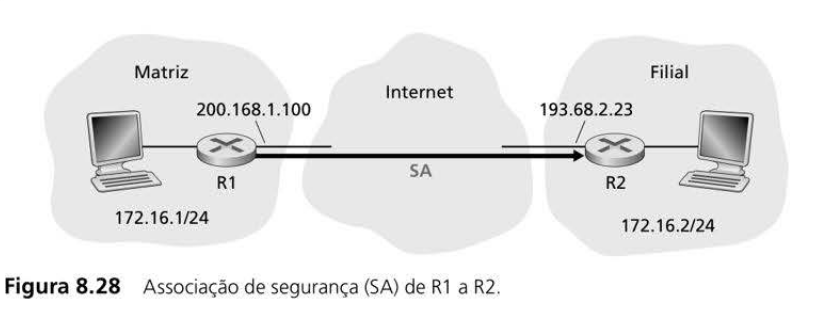
\includegraphics[width=0.7\textwidth]{Figuras/ipsec-e-SAs.png}
    \end{figure}



\end{frame}

\begin{frame}{Uso das Informações de Estado da SA (Exemplo R1 $\rightarrow$ R2)}
    \begin{itemize}
        \item \textbf{No Remetente (Roteador R1)}
              \begin{itemize}
                  \item Quando R1 precisa construir um datagrama IPsec para encaminhar por essa SA:
                  \item Ele acessa as informações de estado (SPI, chaves, algoritmos) da SA.
                  \item Usa essas informações para determinar como deve \textbf{autenticar} e \textbf{criptografar} o datagrama.
              \end{itemize}

        \item \textbf{No Destinatário (Roteador R2)}
              \begin{itemize}
                  \item R2 mantém as \textit{mesmas} informações de estado sobre essa SA (identificada pelo SPI).
                  \item Ele as usa para \textbf{autenticar} (verificar a integridade) e \textbf{decodificar} (descriptografar) qualquer datagrama IPsec que chegar da SA.
              \end{itemize}
    \end{itemize}
\end{frame}

\begin{frame}{Informações de Estado da SA (Exemplo: Roteador RI)}

    O Roteador R1 manterá as informações de estado sobre essa SA:

    \begin{itemize}
        \item Um identificador de 32 bits para a SA: \textbf{Índice de Parâmetro de Segurança (SPI)}


        \item As interfaces da SA:
              \begin{itemize}
                  \item Interface remetente (Origem): 200.168.1.100
                  \item Interface destinatária (Destino): 193.68.2.23
              \end{itemize}

        \item Parâmetros de Criptografia (para Sigilo):
              \begin{itemize}
                  \item O tipo de criptografia (ex: 3DES com CBC).
                  \item A chave de criptografia.
              \end{itemize}

        \item Parâmetros de Integridade (para Autenticação):
              \begin{itemize}
                  \item O tipo de verificação de integridade (ex: HMAC com MD5).
                  \item A chave de autenticação.
              \end{itemize}
    \end{itemize}
\end{frame}

\begin{frame}{Parâmetros da SA (Parte 1)}
    \begin{itemize}
        \item \textbf{Contador de Número de Sequência (Sequence number counter)}
              \begin{itemize}
                  \item Um valor de 32 bits usado para gerar o campo "Sequence Number" nos cabeçalhos AH ou ESP
                  \item Essencial para o antireplay.
              \end{itemize}

        \item \textbf{Estouro do Contador (Sequence counter overflow)}
              \begin{itemize}
                  \item Uma "flag" que indica se o estouro (overflow) do contador deve:
                        \begin{itemize}
                            \item Gerar um evento auditável (log).
                            \item Impedir a transmissão de mais pacotes nesta SA.
                        \end{itemize}
              \end{itemize}

        \item \textbf{Janela Antireplay (Antireplay window)}
              \begin{itemize}
                  \item Define uma "janela deslizante" (sliding window).
                  \item Usada para determinar se um pacote AH ou ESP recebido é um \textit{replay} (pacote duplicado/malicioso).
                  \item O número de sequência do pacote deve estar dentro desta janela.
              \end{itemize}
    \end{itemize}
\end{frame}

\begin{frame}{Parâmetros da SA (Parte 2)}
    \begin{itemize}

        \item \textbf{Informações ESP}
              \begin{itemize}
                  \item Algoritmo de criptografia e autenticação.
                  \item Chaves, Valores de Inicialização (IVs), tempos de vida das chaves e parâmetros relacionados ao ESP.
              \end{itemize}

        \item \textbf{Tempo de Vida da SA (Lifetime)}
              \begin{itemize}
                  \item Um intervalo de tempo ou uma contagem de bytes.
                  \item Após atingido, a SA deve ser substituída por uma nova SA (e novo SPI) ou terminada.
              \end{itemize}

        \item \textbf{Modo do Protocolo IPsec (Protocol mode)}
              \begin{itemize}
                  \item Define o modo de operação: Túnel (Tunnel) ou Transporte (Transport)
              \end{itemize}

        \item \textbf{Path MTU}
              \begin{itemize}
                  \item Armazena o "Maximum Transmission Unit" (tamanho máximo do pacote) observado no caminho.
                  \item Usado para evitar fragmentação de pacotes.
                  \item Inclui variáveis de "envelhecimento" (aging).
              \end{itemize}
    \end{itemize}
\end{frame}

\begin{frame}{O Datagrama IPsec: Modo Túnel vs. Modo Transporte}
    \begin{itemize}
        \item Analisando o datagrama IPsec.

        \item O IPsec possui \textbf{duas formas diferentes de pacotes} (dois modos de operação):
              \begin{itemize}
                  \item \textbf{Modo Túnel (Tunnel Mode)}
                  \item \textbf{Modo Transporte (Transport Mode)}
              \end{itemize}

        \item \textbf{Comparação de Uso:}
              \begin{itemize}
                  \item O \textbf{Modo Túnel} é o mais apropriado para o cenário de VPNs (que vimos anteriormente).
                  \item Por esta razão, o Modo Túnel é \textbf{mais implementado} do que o Modo Transporte.
              \end{itemize}

        \item \textbf{Foco da Aula:}
              \begin{itemize}
                  \item A partir de agora vamos nos concentrar \textbf{exclusivamente no Modo Túnel}.
                  \item (Uma vez que se tem uma compreensão sólida do Modo Túnel, é fácil aprender o Modo Transporte).
              \end{itemize}
    \end{itemize}
\end{frame}
\begin{frame}{Processo de Criação do Datagrama ESP (Modo Túnel)  - Parte 1}
    O processo de encapsulamento (ex: no roteador de borda) segue estes passos
    \begin{itemize}


        \item \textbf{1. Criptografia e criação da mensagem}
              \begin{itemize}
                  \item Pega-se o datagrama IP original (que será protegido).
                  \item Criptografa-se este datagrama (ele se torna o campo "Payload Data").
                  \item Anexa-se na frente dele o "Cabeçalho ESP" (SPI + Seq. Number).
                  \item O pacote resultante é o Cabeçalho ESP + Carga Criptografada + Trailers ESP.
              \end{itemize}

        \item \textbf{2. Autenticação (MAC/ICV)}
              \begin{itemize}
                  \item Cria-se uma autenticação MAC (ou ICV - Integrity Check Value) sobre o datagrama inteiro.
                  \item Utiliza-se o algoritmo (ex: HMAC) e a chave de autenticação especificados na SA.
              \end{itemize}
    \end{itemize}
\end{frame}
\begin{frame}{Processo de Criação do Datagrama ESP (Modo Túnel) - Parte 2}
    \begin{itemize}

        \item \textbf{3. Formação da Carga Útil (Payload) ESP}
              \begin{itemize}
                  \item Anexa-se o MAC (ICV) atrás do datagrama.
                  \item O resultado (Cabeçalho ESP + Carga Criptografada + Trailers + MAC) forma a \textbf{Carga Útil ESP} completa.
              \end{itemize}

        \item \textbf{4. Criação do Novo Cabeçalho IP (Modo Túnel)}
              \begin{itemize}
                  \item Por fim, cria-se um \textbf{novo cabeçalho IP} (IPv4 clássico, 20 bytes).
                  \item Este novo cabeçalho é anexado \textbf{antes} da Carga Útil ESP.
                  \item Este é o cabeçalho que os roteadores da Internet irão ler.
              \end{itemize}
    \end{itemize}
\end{frame}

\begin{frame}{Datagrama IPSec}


    \begin{figure}
        \centering
        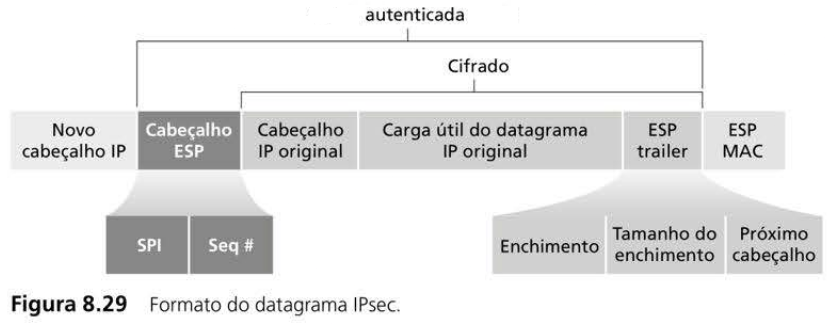
\includegraphics[width=0.9\textwidth]{Figuras/datagrama-ipsec.png}


    \end{figure}



\end{frame}



\begin{frame}{O Datagrama IPsec Resultante (Modo Túnel)}
    \begin{itemize}


        \item \textbf{A Carga Útil (Payload) deste datagrama contém:}
              \begin{itemize}
                  \item O Cabeçalho ESP (SPI, Seq. Number).
                  \item O \textbf{Datagrama IP Original} (cifrado).
                  \item O Trailer ESP (Padding, Pad Length, Next Header) (cifrado).
                  \item O Campo de Autenticação ESP (ICV/MAC).
              \end{itemize}

        \item \textbf{Cabeçalho IP Original (Interno e Cifrado)}
              \begin{itemize}
                  \item Contém os endereços dos \textit{hospedeiros finais}.
                  \item Endereço IP Remetente (Ex): \texttt{172.16.1.17}
                  \item Endereço IP Destinatário (Ex): \texttt{172.16.2.48}
                  \item Estes endereços são \textbf{cifrados} e invisíveis para a Internet.
              \end{itemize}

        \item \textbf{Novo Cabeçalho IP (Externo e Visível)}
              \begin{itemize}
                  \item Contém os endereços das \textit{extremidades do túnel} (os gateways IPsec).
                  \item Endereço IP Remetente (Ex): \texttt{200.168.1.100}
                  \item Endereço IP Destinatário (Ex): \texttt{193.68.2.23}
                  \item O campo "Protocolo" deste novo cabeçalho é \textbf{50} (indicando ESP), e não TCP(6) ou UDP(17).
              \end{itemize}
    \end{itemize}
\end{frame}

\begin{frame}{Revisão: O Cabeçalho ESP (Enviado em Aberto)}
    \begin{itemize}
        \item O "Cabeçalho ESP" é anexado na frente da unidade cifrada (payload + trailer).
        \item Este cabeçalho \textbf{não é criptografado} (é enviado "em aberto" / "clear text").
        \item Ele consiste em dois campos principais:

        \item \textbf{1. O Índice de Parâmetro de Segurança (SPI)}
              \begin{itemize}
                  \item \textbf{Função:} Indica à entidade destinatária (ex: R2) a qual Associação de Segurança (SA) este datagrama pertence.
                  \item \textbf{Ação no Destino:} A entidade usa o SPI para indexar (localizar) rapidamente a SA correta em seu Banco de Dados (SAD).
                  \item Ao localizar a SA, o destino sabe quais algoritmos e chaves deve usar para autenticar e decriptar o pacote.
              \end{itemize}

        \item \textbf{2. O Campo de Número de Sequência}
              \begin{itemize}
                  \item \textbf{Função:} É usado para a proteção contra ataques de repetição (replay attacks).
                  \item (O destinatário verifica este número contra a sua "janela antireplay" definida na SA).
              \end{itemize}
    \end{itemize}
\end{frame}

\begin{frame}{O Trailer ESP: Campos e Criptografia}
    \begin{itemize}
        \item O trailer ESP consiste em três campos:
        \item \textbf{Importante:} O trailer é adicionado ao datagrama IP original \textbf{antes} da cifragem.

        \item \textbf{1. Enchimento (Padding)}
              \begin{itemize}
                  \item \textbf{O quê:} Bytes sem significado.
                  \item \textbf{Por quê:} Cifras de bloco exigem que a mensagem a ser cifrada seja um múltiplo inteiro do comprimento de bloco (ex: 128 bits para o AES).
                  \item O enchimento é usado para "completar" o bloco.
              \end{itemize}

        \item \textbf{2. Tamanho do Enchimento (Pad Length)}
              \begin{itemize}
                  \item \textbf{O quê:} Um campo que indica quantos bytes de enchimento (\textit{padding}) foram inseridos.
                  \item \textbf{Por quê:} Permite à entidade destinatária saber exatamente quanto enchimento deve remover após a decriptação.
              \end{itemize}

        \item \textbf{3. Próximo Cabeçalho (Next Header)}
              \begin{itemize}
                  \item \textbf{O quê:} Identifica o tipo de dados da carga útil (o datagrama original).
                  \item \textbf{Por quê:} Informa ao S.O. do destinatário para qual protocolo entregar o pacote decriptado (ex: TCP, UDP, ICMP).
              \end{itemize}

        \item \textbf{Resumo do Processo de Cifragem:}
              \begin{itemize}
                  \item Os [Dados da Carga Útil (Datagrama IP original)] e o [Trailer ESP] são concatenados.
                  \item O resultado concatenado é então \textbf{cifrado} como uma única unidade.
              \end{itemize}
    \end{itemize}
\end{frame}

\begin{frame}{O MAC de Autenticação ESP (ICV)}
    \begin{itemize}
        \item Além da criptografia, a entidade remetente anexa uma \textbf{Autenticação MAC} (MAC - Message Authentication Code) ou ICV.

        \item \textbf{Sobre o que o MAC é calculado?}
              \begin{itemize}
                  \item O remetente calcula o MAC sobre \textbf{toda o datagrama}.
              \end{itemize}

        \item \textbf{O que  o cálculo do MAC?}
              \begin{itemize}
                  \item O Cabeçalho ESP (SPI + Seq. Number) - (em aberto).
                  \item O Datagrama IP original (já criptografado).
                  \item O Trailer ESP (Padding, etc.) (já criptografado).
              \end{itemize}

        \item \textbf{Como o MAC é calculado? (Revisão)}
              \begin{itemize}
                  \item O remetente anexa uma \textbf{chave MAC secreta} definida na SA.
                  \item Em seguida, calcula um \textbf{hash de tamanho fixo} do resultado (ex: HMAC-MD5 ou HMAC-SHA1).
                  \item Este hash é o MAC/ICV, que é anexado ao final do pacote.
              \end{itemize}
    \end{itemize}
\end{frame}

\begin{frame}{Processamento no Destino (Exemplo: Roteador R2)}
    \begin{itemize}
        \item Quando R2 recebe o datagrama IPsec (destino: R2, protocolo: 50):

        \item \textbf{1. Identificação da SA:}
              \begin{itemize}
                  \item R2 entende que é um pacote ESP (Protocolo 50).
                  \item Ele lê o campo \textbf{SPI} (no cabeçalho ESP) para determinar a qual SA o datagrama pertence (procurando no SAD).
              \end{itemize}

        \item \textbf{2. Verificação de Autenticidade/Integridade:}
              \begin{itemize}
                  \item R2 calcula o MAC sobre o datagrama (usando a chave da SA).
                  \item Compara o MAC calculado com o valor no campo MAC ESP.
                  \item Se forem compatíveis: R2 sabe que (A) o pacote veio de R1 e (B) não foi adulterado.
              \end{itemize}

        \item \textbf{3. Verificação Antireplay:}
              \begin{itemize}
                  \item R2 verifica o campo \textbf{Número de Sequência} para garantir que o datagrama é novo (e não um pacote repetido).
              \end{itemize}
    \end{itemize}
\end{frame}
\begin{frame}{Processamento no Destino (Exemplo: Roteador R2)}
    \begin{itemize}
        \item \textbf{4. Decodificação (Descriptografia):}
              \begin{itemize}
                  \item R2 decodifica a unidade cifrada (payload + trailer) usando o algoritmo e a chave de criptografia da SA.
              \end{itemize}

        \item \textbf{5. Extração do Pacote Original:}
              \begin{itemize}
                  \item R2 remove o enchimento (padding) e extrai o datagrama IP original (que estava cifrado).
              \end{itemize}

        \item \textbf{6. Encaminhamento:}
              \begin{itemize}
                  \item R2 finalmente encaminha o datagrama IP original (agora em claro) para a rede da filial, em direção ao seu destino final (ex: 172.16.2.48).
              \end{itemize}
    \end{itemize}
\end{frame}

\begin{frame}{IKE: Gerenciamento de Chave no IPsec}
    \begin{itemize}
        \item \textbf{O Desafio: Como criar as Associações de Segurança (SAs)?}

        \item \textbf{Opção 1: "Teclagem Manual" (Manual Keying)}
              \begin{itemize}
                  \item \textbf{Cenário:} VPNs com um número pequeno de pontos finais (ex: 2 roteadores).
                  \item \textbf{Ação:} O administrador de rede pode inserir \textit{manualmente} as informações da SA (algoritmos, chaves, SPIs) nos SADs das entidades.
              \end{itemize}

        \item \textbf{O Problema desta Abordagem:}
              \begin{itemize}
                  \item É claramente \textbf{impraticável} para uma VPN grande.
                  \item (Ex: Redes com centenas ou milhares de roteadores e hospedeiros IPsec).
              \end{itemize}

        \item \textbf{Opção 2: O Mecanismo Automático (IKE)}
              \begin{itemize}
                  \item Implementações grandes e geograficamente distribuídas exigem um mecanismo automático para a criação das SAs.
                  \item O IPsec utiliza para isso o protocolo \textbf{IKE (Internet Key Exchange)}.
                  \item Especificado na \textbf{RFC 5996}.
              \end{itemize}
    \end{itemize}
\end{frame}

\begin{frame}{IKE: Funções Principais do Protocolo}
    \begin{itemize}
        \item O protocolo IKE (Internet Key Exchange) é o mecanismo automático para criar SAs.
        \item \textbf{Responsabilidades do IKE:}

        \item \textbf{1. Autenticação das Entidades}
              \begin{itemize}
                  \item Troca certificados para provar a identidade das partes (ex: R1 e R2).
              \end{itemize}

        \item \textbf{2. Negociação de Parâmetros}
              \begin{itemize}
                  \item Negocia os algoritmos de criptografia (ex: AES, 3DES).
                  \item Negocia os algoritmos de autenticação (ex: HMAC-SHA1).
              \end{itemize}

        \item \textbf{3. Geração de Chaves}
              \begin{itemize}
                  \item Troca informações de chave com segurança (usando Diffie-Hellman).
                  \item Cria as chaves de sessão (secretas) que serão usadas nas SAs do IPsec.
              \end{itemize}
    \end{itemize}
\end{frame}

\begin{frame}{IKE: A Estrutura de Duas Fases}
    \begin{itemize}
        \item O IKE opera em duas fases principais (contexto: R1 e R2).

        \item \textbf{Fase 1: O Canal Seguro}
              \begin{itemize}
                  \item Objetivo: Criar um canal seguro e autenticado \textbf{para o próprio IKE}.
                  \item Consiste em duas trocas de pares de mensagens.
                  \item Resultado: Criação de uma \textbf{IKE SA} (bidirecional).
              \end{itemize}

        \item \textbf{Atenção: IKE SA $\neq$ IPsec SA}
              \begin{itemize}
                  \item A \textbf{IKE SA} (Fase 1) é um canal seguro para proteger as negociações do IKE.
                  \item As \textbf{IPsec SAs} (Fase 2) são as conexões unidirecionais usadas para proteger os dados do usuário (o tráfego da VPN).
              \end{itemize}
    \end{itemize}
\end{frame}

\begin{frame}{IKE: Detalhes da Fase 1}
    \begin{itemize}
        \item \textbf{Primeira Troca de Mensagens (Anônima)}
              \begin{itemize}
                  \item Os dois lados (R1, R2) usam \textbf{Diffie-Hellman}.
                  \item \textbf{Objetivo:} Criar a IKE SA bidirecional.
                  \item Chaves são estabelecidas para criptografia e autenticação \textbf{da IKE SA}.
                  \item Um \textbf{segredo mestre} é estabelecido (para ser usado na Fase 2).
                  \item \textit{Importante:} Nesta etapa, nem R1 nem R2 revelam sua identidade (não assinam nada com chaves privadas).
              \end{itemize}

        \item \textbf{Segunda Troca de Mensagens (Autenticada)}
              \begin{itemize}
                  \item Ambos os lados \textbf{revelam suas identidades} (ex: certificados) assinando as mensagens.
                  \item \textit{Segurança:} As identidades não são expostas a "analisadores passivos", pois esta troca já ocorre \textbf{dentro do canal seguro IKE SA} criado na primeira troca.
                  \item \textit{Negociação:} Os dois lados negociam os algoritmos de autenticação e criptografia que serão usados pelas futuras \textbf{SAs IPsec} (da Fase 2).
              \end{itemize}
    \end{itemize}
\end{frame}

\begin{frame}{IKE: Fase 2 e a Motivação}
    \begin{itemize}
        \item \textbf{IKE Fase 2: Criação das SAs IPsec}
              \begin{itemize}
                  \item Ao fim da Fase 1, existe um canal IKE SA seguro e autenticado.
                  \item Na Fase 2, os dois lados usam este canal para criar as \textbf{SAs do IPsec}.
                  \item Criam uma SA IPsec em cada direção (duas SAs unidirecionais).
                  \item As chaves de sessão de criptografia e autenticação são estabelecidas para ambas as SAs IPsec.
                  \item Agora, podem usar essas SAs IPsec para enviar dados seguros.
              \end{itemize}

        \item \textbf{A Motivação para as Duas Fases}
              \begin{itemize}
                  \item \textbf{Custo Computacional.}
                  \item A Fase 1 é "cara" (envolve criptografia de chave pública: Diffie-Hellman e assinaturas RSA).
                  \item A Fase 2 é "barata" (não envolve chave pública; usa o segredo mestre da Fase 1).
                  \item \textbf{Vantagem:} Permite criar um \textit{grande número} de SAs IPsec (Fase 2) com um custo computacional relativamente pequeno, após estabelecer apenas uma IKE SA (Fase 1).
              \end{itemize}
    \end{itemize}
\end{frame}
%\title{Aula 13 - TLS}

\author{Prof. Gabriel Rodrigues Caldas de Aquino}

\institute
{
    Instituto de Computação \\
    Universidade Federal do Rio de Janeiro\\
    gabrielaquino@ic.ufrj.br% Your institution for the title page
}
\date{Compilado em: \\ \today} % Date, can be changed to a custom date

%----------------------------------------------------------------------------------------
%    PRESENTATION SLIDE
%----------------------------------------------------------------------------------------



\begin{frame}
    % Print the title page as the first slide
    \titlepage
\end{frame}

\begin{frame}{Protegendo conexões TCP: TLS}
    \begin{itemize}
        \item \textbf{Contextualização:}
              \begin{itemize}
                  \item Vimos segurança na camada de rede.
                  \item Agora, subimos uma camada na pilha de protocolo.
              \end{itemize}

        \item \textbf{O Objetivo do TLS:}
              \begin{itemize}
                  \item Examinar como a criptografia pode aprimorar o \textbf{TCP}.
                  \item (Transport Layer Security).
              \end{itemize}

        \item \textbf{Serviços de Segurança Adicionados ao TCP:}
              \begin{itemize}
                  \item Sigilo (Confidencialidade).
                  \item Integridade dos Dados.
                  \item Autenticação do Ponto Final (End-point Authentication).
              \end{itemize}

        \item \textbf{Padronização e Histórico:}
              \begin{itemize}
                  \item O TLS é padronizado pelo IETF na \textbf{RFC 4346}.
                  \item Uma versão anterior e semelhante deste protocolo é o \textbf{SSL (Secure Sockets Layer)} versão 3.
              \end{itemize}
    \end{itemize}
\end{frame}

\begin{frame}{TLS: Histórico e Adoção}
    \begin{itemize}
        \item \textbf{Origem:} O SSL (Secure Sockets Layer) foi originalmente projetado pela Netscape.
              \begin{itemize}
                  \item (Ideias básicas sobre proteção do TCP antecedem este trabalho, ex: Woo, 1994).
              \end{itemize}

        \item \textbf{Sucessor:} O TLS (Transport Layer Security) é o sucessor padronizado do SSL.

        \item \textbf{Adoção Massiva:}
              \begin{itemize}
                  \item Suportado por todos os navegadores Web e servidores Web populares.
                  \item Usado pelo Gmail e por \textbf{basicamente todos os sites de comércio eletrônico} (Amazon, eBay, TaoBao).
                  \item Centenas de bilhões de dólares são gastos anualmente usando TLS.
              \end{itemize}

        \item \textbf{Como o usuário identifica o TLS?}
              \begin{itemize}
                  \item Se você já comprou algo online com cartão de crédito, sua comunicação foi quase certamente via TLS.
                  \item A URL no navegador se inicia com \textbf{https://} (em vez de http://).
              \end{itemize}
    \end{itemize}
\end{frame}

\begin{frame}{A Necessidade do TLS: Cenário de E-commerce}
    \begin{itemize}
        \item \textbf{O Cenário Típico:}
              \begin{itemize}
                  \item \textbf{Bob} (cliente) está navegando na Web.
                  \item Ele acessa o site da \textbf{Alice Incorporated} (vendedor) para comprar perfume.
              \end{itemize}

        \item \textbf{A Ação:}
              \begin{itemize}
                  \item O site exibe um formulário.
                  \item Bob insere informações sensíveis:
                        \begin{itemize}
                            \item Tipo de perfume e quantidade.
                            \item Seu endereço.
                            \item O \textbf{número de seu cartão de crédito}.
                        \end{itemize}
                  \item Bob clica em "Enviar".
              \end{itemize}

        \item \textbf{A Expectativa (sem segurança):}
              \begin{itemize}
                  \item Bob espera receber o perfume e a cobrança correta.
                  \item \textbf{O Risco:} Se nenhuma medida de segurança for tomada, Bob pode ter "surpresas".
              \end{itemize}
    \end{itemize}
\end{frame}

\begin{frame}{Riscos: O Cenário de E-commerce sem TLS}
    \begin{itemize}
        \item \textbf{1. Se nenhuma Confidencialidade (Sigilo) for utilizada:}
              \begin{itemize}
                  \item Um invasor (Trudy) poderia \textbf{interceptar} o pedido.
                  \item Trudy rouba as informações do cartão de crédito de Bob.
                  \item Consequência: O invasor pode fazer compras à custa de Bob.
              \end{itemize}

        \item \textbf{2. Se nenhuma Integridade dos Dados for utilizada:}
              \begin{itemize}
                  \item Um invasor poderia \textbf{modificar} o pedido de Bob em trânsito.
                  \item Ex: Fazer Bob comprar 10x mais frascos de perfume do que o desejado.
              \end{itemize}

        \item \textbf{3. Se nenhuma Autenticação do Servidor for utilizada:}
              \begin{itemize}
                  \item Um servidor (mantido por Trudy) poderia \textbf{se passar} pela Alice Inc., usando o mesmo logotipo.
                  \item Bob insere seus dados no site falso de Trudy.
                  \item Consequência: Trudy fica com o dinheiro e some, ou pratica \textbf{roubo de identidade} (nome, endereço, cartão).
              \end{itemize}
    \end{itemize}
\end{frame}

\begin{frame}{TLS: Além do HTTP e Posição na Pilha}
    \begin{itemize}
        \item \textbf{Uso Comum: HTTPS}
              \begin{itemize}
                  \item Muitas vezes, o TLS é usado para oferecer segurança em transações que ocorrem pelo HTTP.
              \end{itemize}

        \item \textbf{O Verdadeiro Alcance: Qualquer Aplicação TCP}
              \begin{itemize}
                  \item Como o TLS protege o \textbf{TCP}, ele pode ser empregado por \textbf{qualquer aplicação} que execute sobre o TCP (ex: FTP, SMTP, etc.).
              \end{itemize}

        \item \textbf{Interface para o Desenvolvedor (API)}
              \begin{itemize}
                  \item O TLS provê uma Interface de Programação de Aplicações (API) com Sockets, muito semelhante à API de Sockets do TCP.
                  \item Para usar o TLS, a aplicação simplesmente inclui as classes ou bibliotecas SSL/TLS.
              \end{itemize}

        \item \textbf{Localização na Pilha de Protocolos}
              \begin{itemize}
                  \item Tecnicamente, o TLS reside na \textbf{Camada de Aplicação}.
                  \item Do ponto de vista do \textbf{desenvolvedor}, ele é visto como um \textbf{protocolo de transporte} que provê serviços do TCP aprimorados com serviços de segurança.
                  \item (Conforme Figura 8.24: TLS fica entre a Aplicação e o TCP).
              \end{itemize}
    \end{itemize}
\end{frame}

\begin{frame}{TLS e o TCP}


    \begin{figure}
        \centering
        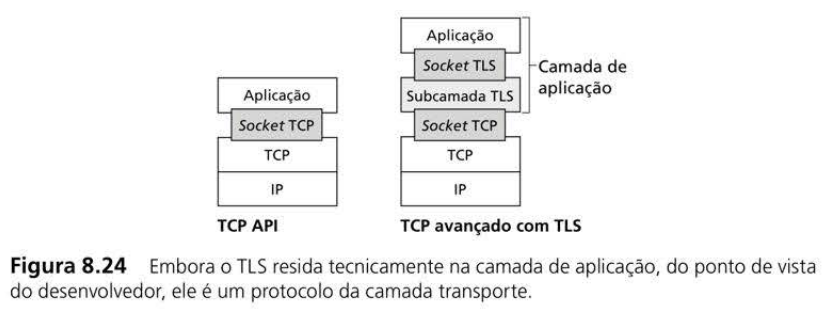
\includegraphics[width=0.9\textwidth]{Figuras/tcp-e-tls.png}


    \end{figure}



\end{frame}

\begin{frame}{Arquitetura do TLS}
    \begin{itemize}
        \item O TLS é projetado para \textbf{usar o TCP} para prover um serviço seguro, confiável (reliable) e fim-a-fim.

        \item O TLS não é um protocolo único, mas sim \textbf{duas camadas} de protocolos.

        \item \textbf{Camada 1: O Protocolo de Registro (Record Protocol)}
              \begin{itemize}
                  \item Fica "em cima" do TCP.
                  \item Fornece os serviços básicos de segurança (criptografia, integridade) para os protocolos da camada superior.
              \end{itemize}

        \item \textbf{Camada 2: Protocolos Superiores (Gerenciamento TLS)}
              \begin{itemize}
                  \item São protocolos \textbf{específicos do TLS}, usados na \textbf{gestão} das trocas TLS.
                  \item São três protocolos que rodam "em cima" do Record Protocol:
                        \begin{itemize}
                            \item Protocolo Handshake (Handshake Protocol)
                            \item Protocolo de Troca de Especificação de Cifra (Change Cipher Spec Protocol)
                            \item Protocolo de Alerta (Alert Protocol)
                        \end{itemize}
              \end{itemize}

        \item \textbf{Camada de Aplicação (Exemplo)}
              \begin{itemize}
                  \item O \textbf{HTTP} (Hypertext Transfer Protocol), usado para interação Web cliente/servidor, pode operar "em cima" do TLS.
              \end{itemize}
    \end{itemize}
\end{frame}

\begin{frame}{A pilha SSL/TLS}


    \begin{figure}
        \centering
        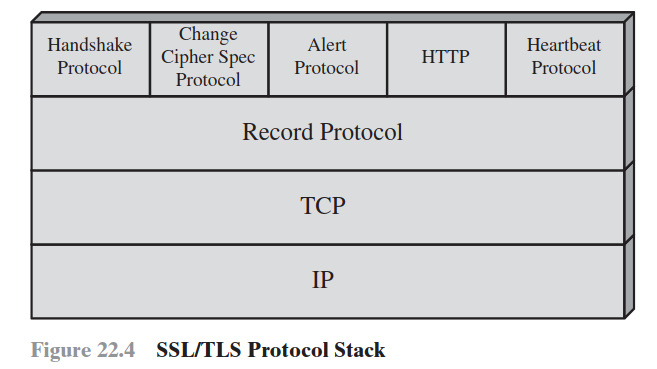
\includegraphics[width=0.7\textwidth]{Figuras/ssl-tls-protocol-stack.png}


    \end{figure}

\end{frame}

\begin{frame}{Conceitos Importantes: Conexão TLS vs. Sessão TLS}
    \begin{itemize}
        \item Existem dois conceitos centrais: Conexão e Sessão.

        \item \textbf{Conexão (Connection)}
              \begin{itemize}
                  \item É um transporte (no sentido OSI) que provê um serviço.
                  \item No TLS, é uma relação \textit{peer-to-peer}.
                  \item As conexões são \textbf{transitórias} (passageiras).
                  \item \textbf{Toda conexão está associada a UMA sessão.}
              \end{itemize}

        \item \textbf{Sessão (Session)}
              \begin{itemize}
                  \item É uma associação entre um cliente e um servidor.
                  \item Criada pelo \textbf{Handshake Protocol}.
                  \item Define um conjunto de \textbf{parâmetros de segurança criptográficos} (chaves, algoritmos, etc.).
                  \item Estes parâmetros podem ser \textbf{compartilhados} entre múltiplas conexões.
                  \item \textbf{Objetivo:} Evitar a negociação (cara) de novos parâmetros de segurança para cada nova conexão.
              \end{itemize}

        \item \textbf{Relacionamento:}
              \begin{itemize}
                  \item Pode haver \textbf{múltiplas conexões seguras} entre um cliente e um servidor.
                  \item Na prática, essas múltiplas conexões compartilham (reutilizam) os parâmetros de uma \textbf{única sessão}.
              \end{itemize}
    \end{itemize}
\end{frame}

\begin{frame}{O protocolo de registro do TLS}


    \begin{figure}
        \centering
        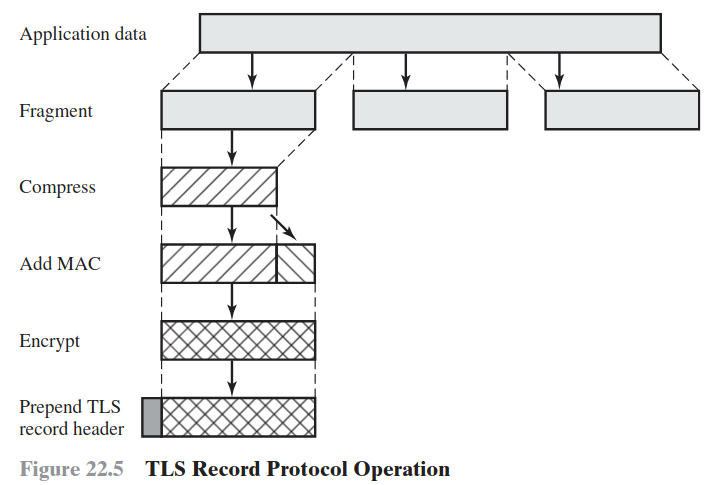
\includegraphics[width=0.7\textwidth]{Figuras/tls-record-protocol.png}


    \end{figure}

\end{frame}

\begin{frame}{Protocolo de Registro TLS (Record Protocol): Serviços}
    \begin{itemize}
        \item O Protocolo de Registro (SSL/TLS Record Protocol) provê dois serviços básicos para as conexões TLS:

        \item \textbf{1. Confidencialidade (Sigilo)}
              \begin{itemize}
                  \item O Protocolo Handshake (visto mais tarde) define uma \textbf{chave secreta compartilhada}.
                  \item Esta chave é usada para \textbf{criptografia simétrica} dos payloads (dados) do TLS.
              \end{itemize}

        \item \textbf{2. Integridade da Mensagem}
              \begin{itemize}
                  \item O Protocolo Handshake também define (outra) \textbf{chave secreta compartilhada}.
                  \item Esta chave é usada para formar um \textbf{MAC (Message Authentication Code)}.
              \end{itemize}

        \item \textbf{Tipos de Conteúdo (Content Types) transportados:}
              \begin{itemize}
                  \item \textit{change\_cipher\_spec} (Protocolo de Gerenciamento TLS)
                  \item \textit{alert} (Protocolo de Gerenciamento TLS)
                  \item \textit{handshake} (Protocolo de Gerenciamento TLS)
                  \item \textit{application\_data} (Dados da Aplicação, ex: HTTP).
              \end{itemize}
        \item \textbf{Obs:} O conteúdo de \textit{application\_data} é \textbf{opaco} para o TLS (ele não sabe o que é HTTP, apenas o protege).
    \end{itemize}
\end{frame}

%\title{Aula 13 - Firewalls}

\author{Prof. Gabriel Rodrigues Caldas de Aquino}

\institute
{
    Instituto de Computação \\
    Universidade Federal do Rio de Janeiro\\
    gabrielaquino@ic.ufrj.br% Your institution for the title page
}
\date{Compilado em: \\ \today} % Date, can be changed to a custom date

%----------------------------------------------------------------------------------------
%    PRESENTATION SLIDE
%----------------------------------------------------------------------------------------



\begin{frame}
    % Print the title page as the first slide
    \titlepage
\end{frame}

\begin{frame}{Firewalls e VPNs}


    \begin{figure}
        \centering
        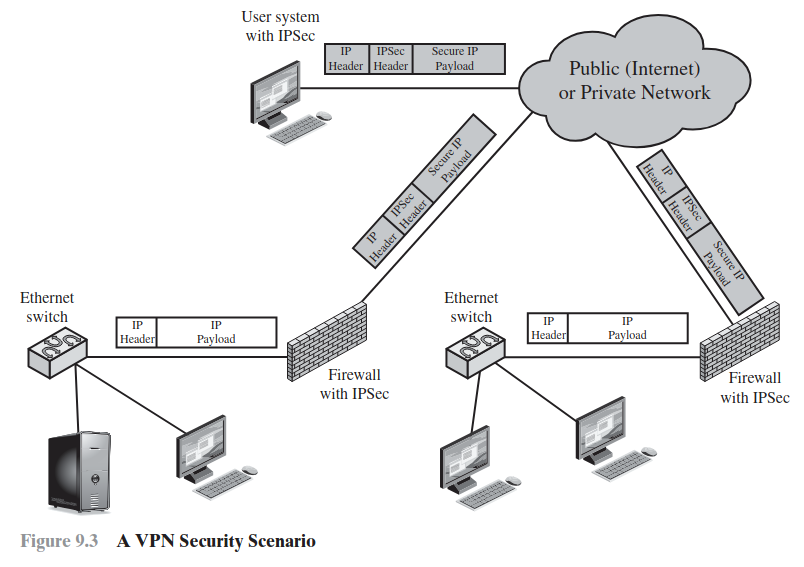
\includegraphics[width=0.7\textwidth]{Figuras/firewalls-vpns.png}


    \end{figure}

\end{frame}

\begin{frame}{O que são Firewalls}
    \begin{itemize}
        \item Firewalls são um meio \textbf{eficaz} de proteger um sistema local ou uma rede contra ameaças de segurança baseadas em rede.

        \item \textbf{O Dilema (O Balanço):}
              \begin{itemize}
                  \item \textbf{Proteger} os ativos internos contra ameaças.
                  \item Ao mesmo tempo, \textbf{permitir} o acesso ao mundo exterior (WANs e Internet).
              \end{itemize}

        \item \textbf{9.1 A Necessidade de Firewalls}
              \begin{itemize}
                  \item A necessidade de firewalls é resultado direto da \textbf{evolução} constante dos sistemas de informação em corporações, agências governamentais e outras organizações.
              \end{itemize}
    \end{itemize}
\end{frame}

\begin{frame}{A Necessidade de Firewalls: Evolução dos Sistemas (Parte 1)}
    \begin{itemize}
        \item Desenvolvimentos notáveis na evolução dos sistemas:

        \item \textbf{1. Sistema Centralizado (Mainframe)}
              \begin{itemize}
                  \item Um mainframe central suportando terminais diretamente conectados.
              \end{itemize}

        \item \textbf{2. Redes Locais (LANs)}
              \begin{itemize}
                  \item Interconectando PCs e terminais entre si e ao mainframe.
              \end{itemize}

        \item \textbf{3. Rede Local Corporativa (Premises Network)}
              \begin{itemize}
                  \item Consiste em várias LANs, interconectando PCs, servidores e (talvez) mainframes.
              \end{itemize}
    \end{itemize}
\end{frame}

\begin{frame}{A Necessidade de Firewalls: Evolução dos Sistemas (Parte 2)}
    \begin{itemize}
        \item Desenvolvimentos notáveis (continuação):

        \item \textbf{4. Rede Corporativa Ampla (Enterprise-wide)}
              \begin{itemize}
                  \item Múltiplas redes locais (premises) geograficamente distribuídas.
                  \item Interconectadas por uma \textbf{WAN privada}.
              \end{itemize}

        \item \textbf{5. Conectividade com a Internet}
              \begin{itemize}
                  \item As várias redes locais (premises) se conectam à Internet (além da WAN privada).
              \end{itemize}

        \item \textbf{6. Computação em Nuvem (Enterprise Cloud)}
              \begin{itemize}
                  \item Servidores virtualizados em data centers.
                  \item Provendo serviços internos (organizacionais) e externos (acessíveis pela Internet).
              \end{itemize}
    \end{itemize}
\end{frame}

\begin{frame}{O Dilema da Conectividade com a Internet}
    \begin{itemize}
        \item \textbf{A Realidade Atual:}
              \begin{itemize}
                  \item A conectividade com a Internet \textbf{não é mais opcional} para a maioria das organizações.
                  \item A informação e os serviços disponíveis são essenciais.
                  \item Usuários internos (indivíduos) precisam e desejam o acesso à Internet.
              \end{itemize}

        \item \textbf{O Problema (A Ameaça):}
              \begin{itemize}
                  \item Embora o acesso à Internet traga benefícios, ele \textbf{permite ao mundo exterior} alcançar e interagir com os ativos da rede local.
                  \item Isso cria uma ameaça significativa para a organização.
              \end{itemize}

        \item \textbf{Por que a Segurança por Máquina não é Suficiente?}
              \begin{itemize}
                  \item É possível equipar cada workstation e servidor com segurança forte (ex: proteção contra intrusão).
                  \item \textbf{Porém:} Isso pode \textbf{não ser suficiente} e, em alguns casos, \textbf{não é custo-efetivo}.
              \end{itemize}
        \item \textbf{Conclusão:} A necessidade de uma solução de perímetro (Firewall).
    \end{itemize}
\end{frame}

\begin{frame}{O Desafio da Segurança Apenas no Hospedeiro (Host-Based)}
    \begin{itemize}
        \item Considere uma rede com centenas ou milhares de sistemas.
              \begin{itemize}
                  \item Executando vários sistemas operacionais (diferentes versões de Windows, MacOS, Linux).
              \end{itemize}

        \item \textbf{O Problema (Desafio de Escala):}
              \begin{itemize}
                  \item Quando uma falha de segurança é descoberta, \textbf{cada} sistema potencialmente afetado deve ser atualizado (patched).
                  \item Isso requer um gerenciamento de configuração escalável e \textit{patching} agressivo para funcionar.
                  \item É difícil, embora possível e necessário se for a \textit{única} defesa.
              \end{itemize}

        \item \textbf{A Alternativa (ou Complemento): O Firewall}
              \begin{itemize}
                  \item Uma alternativa amplamente aceita para os serviços de segurança baseados em host.
              \end{itemize}
    \end{itemize}
\end{frame}

\begin{frame}{Firewall: A Defesa de Perímetro}
    \begin{itemize}
        \item \textbf{Posicionamento:}
              \begin{itemize}
                  \item Inserido \textbf{entre} a rede local (premises) e a Internet.
              \end{itemize}

        \item \textbf{Objetivo Principal:}
              \begin{itemize}
                  \item Estabelecer um \textbf{link controlado}.
                  \item Erguer um "muro" de segurança externo, ou \textbf{perímetro}.
                  \item Proteger a rede local de ataques baseados na Internet.
              \end{itemize}

        \item \textbf{O Conceito de "Ponto de Gargalo" (Choke Point)}
              \begin{itemize}
                  \item Fornece um \textbf{ponto único} onde a segurança e a auditoria podem ser impostas.
              \end{itemize}

        \item \textbf{Implementação:}
              \begin{itemize}
                  \item Pode ser um único sistema de computador.
                  \item Ou um conjunto de dois ou mais sistemas que cooperam.
              \end{itemize}

        \item \textbf{Resultado: Defesa em Profundidade}
              \begin{itemize}
                  \item O firewall fornece uma \textbf{camada adicional de defesa}, isolando os sistemas internos.
                  \item Segue a doutrina militar clássica de "defesa em profundidade" (defense in depth).
              \end{itemize}
    \end{itemize}
\end{frame}

\begin{frame}{Objetivos de Design do Firewall (Segundo [BELL94])}
    \begin{itemize}
        \item \textbf{1. Centralização do Tráfego:}
              \begin{itemize}
                  \item \textbf{Todo} o tráfego (de dentro para fora e vice-versa) \textbf{deve passar} através do firewall.
                  \item \textit{Como isso é alcançado?} Bloqueando fisicamente todo o acesso à rede local, \textbf{exceto} pela via do firewall.
              \end{itemize}

        \item \textbf{2. Controle de Autorização:}
              \begin{itemize}
                  \item \textbf{Apenas} o tráfego autorizado, conforme definido pela \textbf{política de segurança local}, terá permissão para passar.
              \end{itemize}

        \item \textbf{3. Imunidade do Próprio Firewall:}
              \begin{itemize}
                  \item O próprio firewall deve ser \textbf{imune à penetração}.
                  \item \textit{Como isso é alcançado?} Implica o uso de um \textit{hardened system} (sistema reforçado) com um sistema operacional seguro.
              \end{itemize}
    \end{itemize}
\end{frame}

\begin{frame}{O Papel Crítico da Política de Acesso}
    \begin{itemize}
        \item Um componente crítico no planejamento e implementação de um firewall é a especificação de uma \textbf{Política de Acesso} (Access Policy) adequada.

        \item \textbf{O que é a Política de Acesso?}
              \begin{itemize}
                  \item Lista os tipos de tráfego \textbf{autorizados} a passar pelo firewall.
                  \item Define critérios baseados em:
                        \begin{itemize}
                            \item Faixas de endereço (Address ranges)
                            \item Protocolos
                            \item Aplicações
                            \item Tipos de conteúdo (Content types)
                        \end{itemize}
              \end{itemize}

        \item \textbf{Desenvolvimento da Política:}
              \begin{itemize}
                  \item \textbf{Origem:} Deve ser desenvolvida a partir da \textbf{avaliação de risco} (risk assessment) e da política de segurança da informação da organização.
                  \item \textbf{Processo:} Inicia com uma especificação ampla (quais tipos de tráfego a organização \textit{precisa} suportar).
                  \item \textbf{Refinamento:} É então refinada para detalhar os \textbf{elementos de filtro} (filter elements) específicos.
                  \item \textbf{Implementação:} Finalmente, é implementada na topologia de firewall apropriada.
              \end{itemize}
    \end{itemize}
\end{frame}

\begin{frame}{Características da Política de Acesso (NIST SP 800-41) - Parte 1}
    \begin{itemize}
        \item O NIST SP 800-41 lista características que a política de acesso pode usar para filtrar tráfego:

        \item \textbf{Valores de Endereço IP e Protocolo}
              \begin{itemize}
                  \item Controla o acesso com base em: endereços de origem/destino, números de porta, direção do fluxo (inbound/outbound).
                  \item Usado por: \textbf{Filtros de Pacotes} e \textbf{Stateful Inspection Firewalls}.
                  \item Objetivo: Limitar o acesso a serviços específicos.
              \end{itemize}

        \item \textbf{Protocolo da Aplicação}
              \begin{itemize}
                  \item Controla o acesso com base nos dados autorizados do protocolo da aplicação.
                  \item Usado por: \textbf{Application-Level Gateway} (Proxy).
                  \item Ex: Checar e-mail (SMTP) para spam, ou requisições (HTTP) para sites autorizados.
              \end{itemize}
    \end{itemize}
\end{frame}

\begin{frame}{Características da Política de Acesso (NIST SP 800-41) - Parte 2}
    \begin{itemize}
        \item \textbf{Identidade do Usuário (User Identity)}
              \begin{itemize}
                  \item Controla o acesso com base na identidade do usuário.
                  \item Típico para usuários internos (\textit{inside users}).
                  \item Requer autenticação segura (ex: IPsec).
              \end{itemize}

        \item \textbf{Atividade da Rede (Network Activity)}
              \begin{itemize}
                  \item Controla o acesso com base em considerações como:
                        \begin{itemize}
                            \item \textbf{Hora da requisição} (ex: apenas em horário comercial).
                            \item \textbf{Taxa de requisições} (ex: para detectar tentativas de \textit{scanning}).
                            \item Outros padrões de atividade.
                        \end{itemize}
              \end{itemize}
    \end{itemize}
\end{frame}

\begin{frame}{Capacidades do Firewall: O que Esperar}
    \begin{itemize}
        \item \textbf{1. Ponto de Gargalo Único (Single Choke Point)}
              \begin{itemize}
                  \item Tenta manter usuários não autorizados fora da rede.
                  \item Proíbe serviços vulneráveis de entrar ou sair da rede.
                  \item Fornece proteção contra IP spoofing e ataques de roteamento.
                  \item \textit{Vantagem:} Simplifica a gestão de segurança (capacidades consolidadas).
              \end{itemize}

        \item \textbf{2. Localização para Monitoramento}
              \begin{itemize}
                  \item Permite a implementação de auditorias (audits) e alarmes.
              \end{itemize}

        \item \textbf{3. Plataforma para Funções de Internet (Não-Segurança)}
              \begin{itemize}
                  \item \textbf{NAT (Network Address Translator):} Mapeia endereços locais para endereços de Internet.
                  \item \textbf{Gerenciamento de Rede:} Audita ou registra (logs) o uso da Internet.
              \end{itemize}

        \item \textbf{4. Plataforma para IPsec}
              \begin{itemize}
                  \item Pode ser usado para implementar Redes Privadas Virtuais (VPNs).
                  \item Utiliza a capacidade do "modo túnel" (tunnel mode) do IPsec.
              \end{itemize}
    \end{itemize}
\end{frame}

\begin{frame}{Limitações dos Firewalls}
    \begin{itemize}
        \item \textbf{1. Não protege contra ataques que "contornam" (bypass) o firewall.}
              \begin{itemize}
                  \item Sistemas internos podem ter acesso direto a um ISP (ex: banda larga móvel ou com fio).
                  \item LANs internas podem ter conexões diretas com organizações parceiras.
              \end{itemize}

        \item \textbf{2. Não protege totalmente contra ameaças internas.}
              \begin{itemize}
                  \item Ex: Um funcionário insatisfeito (disgruntled employee).
                  \item Ex: Um funcionário que coopera (sem saber) com um atacante externo (ex: phishing).
              \end{itemize}

        \item \textbf{3. LANs sem fio (Wireless) inseguras.}
              \begin{itemize}
                  \item Podem ser acessadas de fora da organização.
                  \item Firewalls internos (separando redes) não podem proteger contra comunicação wireless direta entre sistemas em lados opostos do firewall.
              \end{itemize}

        \item \textbf{4. Dispositivos portáteis infectados (BYOD).}
              \begin{itemize}
                  \item Um laptop, PDA ou dispositivo de armazenamento portátil (pen drive) pode ser usado e infectado \textbf{fora} da rede corporativa.
                  \item E, em seguida, ser conectado e usado \textbf{internamente}, transportando a ameaça.
              \end{itemize}
    \end{itemize}
\end{frame}

\begin{frame}{Firewall genérico}


    \begin{figure}
        \centering
        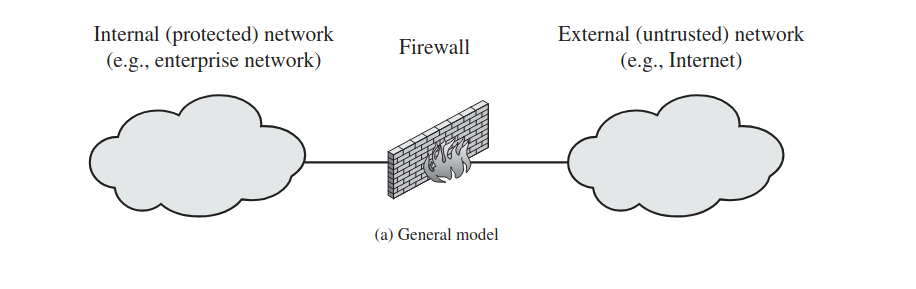
\includegraphics[width=\textwidth]{Figuras/firewall1.png}


    \end{figure}

\end{frame}

\begin{frame}{Tipos de Firewalls}


    \begin{figure}
        \centering
        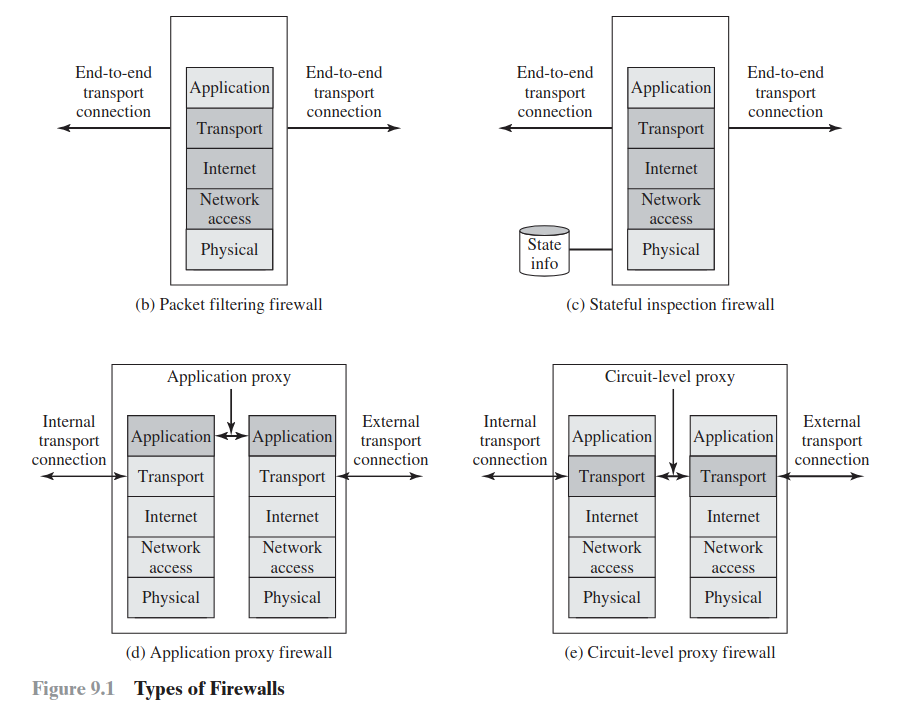
\includegraphics[width=0.7\textwidth]{Figuras/firewall-tipos.png}


    \end{figure}

\end{frame}

\begin{frame}{Introdução: Tipos de Firewalls}
    \begin{itemize}
        \item Um firewall pode monitorar o tráfego de rede em \textbf{vários níveis}:
              \begin{itemize}
                  \item Pacotes de rede de baixo nível (individualmente ou como um fluxo).
                  \item Todo o tráfego dentro de uma conexão de transporte.
                  \item Detalhes dos protocolos de aplicação.
              \end{itemize}

        \item O nível de monitoramento apropriado é determinado pela \textbf{política de acesso} (access policy) desejada.

        \item \textbf{Lógica de Filtragem (Implementa a Política):}
              \begin{itemize}
                  \item \textbf{Filtro Positivo (Positive Filter):} Permite passar \textit{apenas} os pacotes que atendem a critérios específicos.
                  \item \textbf{Filtro Negativo (Negative Filter):} Rejeita \textit{qualquer} pacote que atenda a certos critérios.
              \end{itemize}

        \item \textbf{O que o Firewall Examina (Depende do Tipo):}
              \begin{itemize}
                  \item Um ou mais cabeçalhos de protocolo em cada pacote.
                  \item O \textit{payload} (carga útil) de cada pacote.
                  \item O padrão gerado por uma \textbf{sequência} de pacotes.
              \end{itemize}


    \end{itemize}
\end{frame}

\begin{frame}{Tipo 1: Firewall de Filtro de Pacotes (Definição)}
    \begin{itemize}
        \item Chamado de \textit{Packet Filtering Firewall}.
        \item Aplica um conjunto de regras a \textbf{cada} pacote IP (de entrada e saída).
        \item Ação resultante: \textbf{Encaminhar} (forward) ou \textbf{Descartar} (discard) o pacote.
        \item Tipicamente configurado para filtrar pacotes em \textbf{ambas as direções} (de e para a rede interna).

        \item \textbf{Regras baseadas nas informações do pacote (Camadas 3 e 4):}
              \begin{itemize}
                  \item \textbf{Endereço IP de Origem:} O IP do sistema que originou o pacote.
                  \item \textbf{Endereço IP de Destino:} O IP do sistema que o pacote tenta alcançar.
                  \item \textbf{Porta de Origem/Destino (Nível Transporte):} O número da porta TCP ou UDP (que define aplicações como SNMP ou HTTP).
                  \item \textbf{Campo Protocolo IP:} Define o protocolo de transporte (ex: TCP, UDP, ICMP).
                  \item \textbf{Interface:} Em firewalls com 3+ portas, indica de qual interface o pacote veio ou para qual vai.
              \end{itemize}
    \end{itemize}
\end{frame}

\begin{frame}{Filtro de Pacotes: Lógica de Regras e Políticas Padrão}
    \begin{itemize}
        \item O filtro é configurado como uma \textbf{lista de regras}.
        \item O firewall compara os cabeçalhos (IP/TCP) de cada pacote com esta lista.

        \item \textbf{Se houver correspondência:} A regra é invocada (encaminhar/descartar).
        \item \textbf{Se NÃO houver correspondência:} A \textbf{ação padrão} (default action) é tomada.

        \item \textbf{Duas Políticas Padrão Possíveis:}

        \item \textbf{1. Padrão = Descartar (Default Discard)}
              \begin{itemize}
                  \item "Aquilo que não é expressamente permitido é proibido."
                  \item \textbf{Mais conservadora (segura).}
                  \item Inicialmente, tudo é bloqueado; serviços são adicionados caso a caso.
                  \item Mais visível para usuários (visto como um obstáculo no início).
                  \item Preferida por empresas e governo.
              \end{itemize}

        \item \textbf{2. Padrão = Encaminhar (Default Forward)}
              \begin{itemize}
                  \item "Aquilo que não é expressamente proibido é permitido."
                  \item Aumenta a facilidade de uso para os usuários finais.
                  \item \textbf{Segurança reduzida.}
                  \item O admin deve "reagir" a cada nova ameaça conforme ela se torna conhecida.
                  \item Usada por organizações mais abertas (ex: universidades).
              \end{itemize}
    \end{itemize}
\end{frame}

\begin{frame}{Exemplo de regras de filtragem em Firewalls}


    \begin{figure}
        \centering
        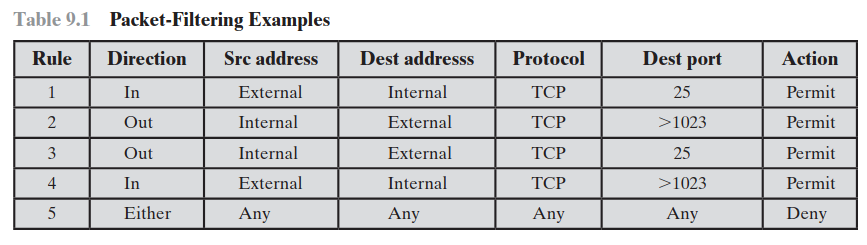
\includegraphics[width=\textwidth]{Figuras/filtragem-de-pacotes.png}


    \end{figure}

\end{frame}

\begin{frame}{Filtro de Pacotes: Exemplo de Regras SMTP (Tabela 9.1)}
    \begin{itemize}
        \item \textbf{Objetivo:} Permitir tráfego de e-mail (SMTP, porta 25) de entrada e saída, mas bloquear todo o resto.
        \item \textbf{Lógica:} Regras aplicadas de cima para baixo (top-to-bottom).

        \item \textbf{Intenção das Regras:}
              \begin{itemize}
                  \item \textbf{Regra 1:} Permitir e-mail \textbf{de entrada} (destino porta 25).
                  \item \textbf{Regra 2:} Permitir a \textbf{resposta} ao e-mail de entrada.
                  \item \textbf{Regra 3:} Permitir e-mail \textbf{de saída} (destino porta 25).
                  \item \textbf{Regra 4:} Permitir a \textbf{resposta} ao e-mail de saída.
                  \item \textbf{Regra 5:} Política padrão (Default = Discard). (Sempre a última regra, explícita ou implicitamente).
              \end{itemize}

        \item \textbf{O Problema (A Falha):}
              \begin{itemize}
                  \item \textbf{A Regra 4 é muito permissiva.} Ela permite tráfego externo para \textbf{qualquer} porta de destino acima de 1023 (assumindo que seja uma "resposta").
              \end{itemize}
    \end{itemize}
\end{frame}

\begin{frame}{Exemplo SMTP: O Exploit e a Solução}
    \begin{itemize}
        \item \textbf{Exemplo de Exploit (usando a Regra 4):}
              \begin{itemize}
                  \item Um atacante externo abre uma conexão da porta 5150 (do atacante) para um Web Proxy interno na porta 8080.
                  \item A Regra 4 (antiga) \textbf{permite} isso, pois a porta de destino (8080) é \> 1023.
                  \item Isso deveria ser proibido e poderia permitir um ataque ao servidor proxy.
              \end{itemize}

        \item \textbf{A Solução (Refinando as Regras):}
              \begin{itemize}
                  \item Configurar o campo de \textbf{porta de origem (source port)} nas regras, tornando-as mais específicas (menos permissivas).
              \end{itemize}

        \item \textbf{Regras Refinadas:}
              \begin{itemize}
                  \item \textbf{Regras 2 e 4 (Respostas):}
                        \begin{itemize}
                            \item Definir a Porta de Origem = \textbf{25}.
                            \item (Pois a resposta a um e-mail deve vir da porta 25 do servidor).
                        \end{itemize}
                  \item \textbf{Regras 1 e 3 (Novas conexões):}
                        \begin{itemize}
                            \item Definir a Porta de Origem = \textbf{\> 1023}.
                            \item (Pois um cliente iniciando um e-mail usará uma porta alta).
                        \end{itemize}
              \end{itemize}
    \end{itemize}
\end{frame}

\begin{frame}{Filtro de Pacotes: Vulnerabilidade Remanescente (SMTP)}
    \begin{itemize}
        \item Mesmo com as regras de porta de origem refinadas, uma vulnerabilidade permanece.

        \item \textbf{A Situação (Regras 3 e 4):}
              \begin{itemize}
                  \item Permitem que qualquer host interno envie e-mail para fora (Porta de Destino = 25).
              \end{itemize}

        \item \textbf{O Problema:}
              \begin{itemize}
                  \item O uso da porta 25 para recebimento de SMTP é apenas um \textbf{padrão} (default).
              \end{itemize}

        \item \textbf{O Risco (O Exploit):}
              \begin{itemize}
                  \item Uma máquina externa (atacante) poderia ser configurada para rodar \textbf{outra aplicação} (maliciosa) na porta 25.
                  \item O atacante poderia então enviar pacotes \textbf{DA} sua porta de origem 25 (TCP Source Port = 25) para tentar invadir máquinas internas.
                  \item A Regra 4 (revisada) permitiria isso, pois ela está configurada para aceitar pacotes \textit{vindos} da porta 25 (assumindo ser uma resposta).
              \end{itemize}
    \end{itemize}
\end{frame}

\begin{frame}{Filtro de Pacotes: A Solução (Flag ACK)}
    \begin{itemize}
        \item \textbf{A Contramedida:}
              \begin{itemize}
                  \item Para combater essa ameaça, podemos adicionar um campo de \textbf{Flag ACK} (ACK flag) à verificação da regra.
              \end{itemize}

        \item \textbf{Onde aplicar:}
              \begin{itemize}
                  \item Esta verificação é adicionada à \textbf{Regra 4} (a regra que permite a \textit{resposta} do servidor externo).
              \end{itemize}

        \item \textbf{A Nova Lógica (Regra 4):}
              \begin{itemize}
                  \item A regra agora exigiria que o \textbf{flag ACK} esteja \textbf{definido} (set) no pacote de entrada.
              \end{itemize}

        \item \textbf{Por que isso funciona?}
              \begin{itemize}
                  \item Um pacote que é parte de uma conexão TCP \textbf{estabelecida} (como uma resposta SMTP legítima) \textbf{SEMPRE} terá o flag ACK definido.
                  \item Um pacote de um atacante tentando \textbf{iniciar} uma nova conexão (o exploit) \textbf{NÃO} teria o flag ACK definido (ex: teria um flag SYN).
              \end{itemize}

        \item A Regra 4 agora se pareceria com:
              \begin{itemize}
                  \item (O texto a seguir deve descrever a nova regra, incluindo a verificação do Flag ACK).
              \end{itemize}
    \end{itemize}
\end{frame}

\begin{frame}{Exemplo de regras de filtragem em Firewalls}


    \begin{figure}
        \centering
        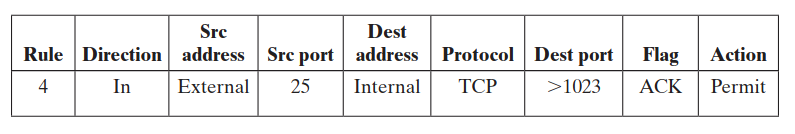
\includegraphics[width=\textwidth]{Figuras/filtro-pacote02.png}


    \end{figure}
    \textbf{A Lógica da Nova Regra:}
    \begin{itemize}
        \item A regra agora permite pacotes de entrada (respostas) que possuem:
              \begin{itemize}
                  \item Porta de Origem (Source Port) = 25
                  \item \textbf{E} o flag ACK definido no segmento TCP.
              \end{itemize}
        \item (Isso efetivamente bloqueia pacotes que \textit{iniciam} conexões (ex: flag SYN) da porta 25, que era a vulnerabilidade.)
    \end{itemize}
\end{frame}

\begin{frame}{Filtro de Pacotes: Vantagens}
    \begin{itemize}
        \item \textbf{1. Simplicidade}
              \begin{itemize}
                  \item A sua lógica de regras é direta (baseada em cabeçalhos L3/L4).
              \end{itemize}

        \item \textbf{2. Transparência}
              \begin{itemize}
                  \item Geralmente são transparentes para os usuários (não exigem configuração no cliente).
              \end{itemize}

        \item \textbf{3. Velocidade}
              \begin{itemize}
                  \item São muito rápidos, pois não inspecionam o payload (carga útil) do pacote.
              \end{itemize}

        \item \textbf{Desvantagens:}
              \begin{itemize}
                  \item O NIST SP 800-41 lista várias fraquezas significativas.
              \end{itemize}
    \end{itemize}
\end{frame}

\begin{frame}{Filtro de Pacotes: Fraquezas (NIST SP 800-41) - Parte 1}
    \begin{itemize}
        \item \textbf{1. Não examina dados da camada superior (Payload)}
              \begin{itemize}
                  \item \textbf{Problema:} Não pode prevenir ataques que usam vulnerabilidades \textbf{específicas da aplicação}.
                  \item \textbf{Exemplo:} Não pode bloquear comandos de aplicação específicos (se o firewall permite a aplicação, todas as funções dela são permitidas).
              \end{itemize}

        \item \textbf{2. Funcionalidade de Log Limitada}
              \begin{itemize}
                  \item \textbf{Problema:} Devido à informação limitada que o firewall vê.
                  \item \textbf{Conteúdo do Log:} Geralmente contém apenas as informações usadas para a decisão (IPs de origem/destino, tipo de tráfego).
              \end{itemize}
    \end{itemize}
\end{frame}

\begin{frame}{Filtro de Pacotes: Fraquezas (NIST SP 800-41) - Parte 2}
    \begin{itemize}
        \item \textbf{3. Não suporta autenticação avançada de usuário}
              \begin{itemize}
                  \item \textbf{Problema:} Novamente, devido à falta de funcionalidade de camada superior.
              \end{itemize}

        \item \textbf{4. Vulnerável a ataques contra a pilha TCP/IP}
              \begin{itemize}
                  \item \textbf{Exemplo:} \textit{Network layer address spoofing} (falsificação de endereço IP).
                  \item \textbf{Problema:} Muitos filtros não conseguem detectar um pacote onde a informação de endereçamento (Camada 3) foi alterada.
                  \item \textbf{Uso:} Usado por intrusos para "burlar" (bypass) os controles do firewall.
              \end{itemize}

        \item \textbf{5. Suscetível a configurações incorretas (Misconfiguration)}
              \begin{itemize}
                  \item \textbf{Problema:} Devido ao pequeno número de variáveis usadas nas decisões.
                  \item \textbf{Risco:} É fácil configurar acidentalmente o firewall para permitir tráfego que deveria ser negado.
              \end{itemize}
    \end{itemize}
\end{frame}

\begin{frame}{Ataques ao Filtro de Pacotes: IP Address Spoofing}
    \begin{itemize}
        \item \textbf{O Ataque (IP Address Spoofing):}
              \begin{itemize}
                  \item O intruso transmite pacotes \textbf{de fora} da rede.
                  \item O campo "Source IP Address" (IP de Origem) é falsificado (spoofed) para conter o endereço de um \textbf{host interno} confiável.
              \end{itemize}

        \item \textbf{O Objetivo:}
              \begin{itemize}
                  \item Penetrar sistemas que empregam segurança simples baseada no endereço de origem (ex: "aceitar pacotes vindos de IPs internos confiáveis").
              \end{itemize}

        \item \textbf{A Contramedida:}
              \begin{itemize}
                  \item O firewall (ou roteador externo) deve \textbf{descartar} pacotes se:
                        \begin{itemize}
                            \item O pacote chega na interface \textbf{externa}.
                            \item \textbf{E} o pacote possui um endereço de origem (source address) \textbf{interno}.
                        \end{itemize}
              \end{itemize}
    \end{itemize}
\end{frame}



\begin{frame}{Ataques ao Filtro de Pacotes: Tiny Fragment}
    \begin{itemize}
        \item \textbf{O Ataque (Tiny Fragment Attack):}
              \begin{itemize}
                  \item O intruso usa a opção de fragmentação IP para criar \textbf{fragmentos extremamente pequenos}.
                  \item \textbf{Objetivo:} Forçar o cabeçalho TCP (que contém as portas) para um \textbf{fragmento separado} (ex: o segundo fragmento), deixando o primeiro fragmento apenas com o cabeçalho IP.
              \end{itemize}

        \item \textbf{A Lógica do Ataque:}
              \begin{itemize}
                  \item O filtro de pacotes toma sua decisão (Permitir/Negar) com base no \textbf{primeiro fragmento}.
                  \item O atacante espera que o primeiro fragmento (incompleto) seja permitido, e que os fragmentos subsequentes (com o TCP malicioso) passem direto.
              \end{itemize}

        \item \textbf{A Contramedida:}
              \begin{itemize}
                  \item Reforçar uma regra de que o \textbf{primeiro fragmento} de um pacote \textbf{deve conter} uma quantidade mínima predefinida do cabeçalho de transporte (TCP).
                  \item (Se o primeiro fragmento for rejeitado, o filtro deve memorizar o ID do pacote e descartar todos os fragmentos subsequentes).
              \end{itemize}
    \end{itemize}
\end{frame}

\begin{frame}{O Problema do Filtro de Pacotes (Falta de Contexto)}
    \begin{itemize}
        \item Um filtro de pacotes tradicional (stateless) toma decisões \textbf{pacote a pacote}.
        \item Ele \textbf{não considera o contexto} de camada superior (se uma conexão TCP existe).

        \item \textbf{Contexto (Modelo Cliente/Servidor):}
              \begin{itemize}
                  \item Aplicações (ex: SMTP) usam TCP.
                  \item \textbf{Servidor (ex: SMTP):} Usa uma "porta bem conhecida" (well-known), que é fixa e < 1024 (ex: Porta \textbf{25}).
                  \item \textbf{Cliente (ex: usuário):} Usa uma porta dinâmica, temporária e > 1024 (ex: Porta \textbf{49152}).
              \end{itemize}

        \item \textbf{A Vulnerabilidade do Filtro de Pacotes:}
              \begin{itemize}
                  \item Para permitir o tráfego de \textit{resposta} (do servidor na porta 25 para o cliente na porta 49152), o firewall deve permitir tráfego de entrada em \textbf{TODAS} as portas altas (>1023).
                  \item Isso cria uma vulnerabilidade enorme que pode ser explorada por atacantes.
              \end{itemize}
    \end{itemize}
\end{frame}

\begin{frame}{Tipo 2: Firewall de Inspeção de Estado (Stateful)}
    \begin{itemize}
        \item (Stateful Packet Inspection Firewall).
        \item \textbf{A Solução:} "Aperta" as regras para o tráfego TCP.

        \item \textbf{O Mecanismo (O "Estado"):}
              \begin{itemize}
                  \item O firewall cria e mantém um \textbf{diretório (Tabela de Estado)} das conexões TCP de \textit{saída} (outbound) que estão ativas.
                  \item (Ref: Tabela 9.2).
                  \item Uma entrada é criada para cada conexão atualmente estabelecida.
              \end{itemize}

        \item \textbf{A Nova Lógica de Filtragem:}
              \begin{itemize}
                  \item O firewall agora permite tráfego de entrada em portas altas (>1023) \textbf{APENAS} se este pacote \textbf{corresponder} (fit the profile) a uma das entradas (conexões) existentes no diretório (Tabela de Estado).
              \end{itemize}
    \end{itemize}
\end{frame}

\begin{frame}{Firewall de Inspeção de Estado (Capacidades)}
    \begin{itemize}
        \item Um firewall stateful revisa as mesmas informações que um filtro de pacotes (cabeçalhos L3/L4).

        \item \textbf{MAS TAMBÉM...}
              \begin{itemize}
                  \item Registra informações sobre o \textbf{estado da conexão TCP} (ex: estabelecida, fechando, etc.).
              \end{itemize}

        \item \textbf{Recursos Avançados (em alguns firewalls stateful):}
              \begin{itemize}
                  \item \textbf{Rastreamento de Números de Sequência TCP:}
                        \begin{itemize}
                            \item Usado para prevenir ataques que dependem do número de sequência (ex: \textit{session hijacking}).
                        \end{itemize}
                  \item \textbf{Inspeção Limitada de Aplicação (Deep Packet Inspection - DPI):}
                        \begin{itemize}
                            \item Inspecionam (de forma limitada) os dados da aplicação.
                            \item Útil para protocolos "problemáticos" (ex: FTP, IM, SIPS) para identificar e rastrear conexões de dados relacionadas.
                        \end{itemize}
              \end{itemize}
    \end{itemize}
\end{frame}

\begin{frame}{Filtro de pacotes com estado}


    \begin{figure}
        \centering
        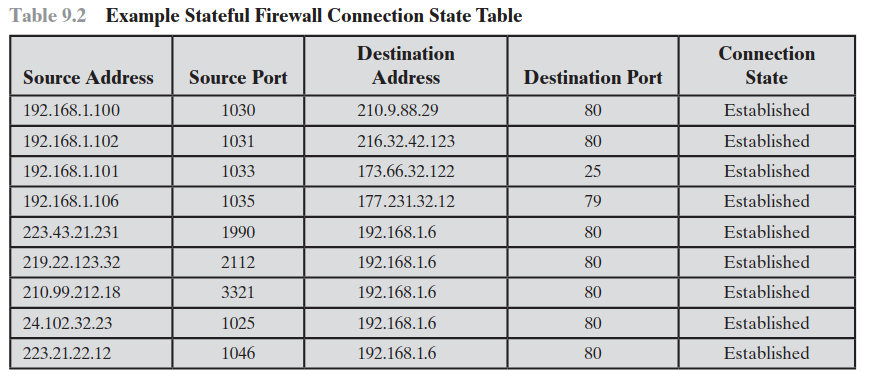
\includegraphics[width=\textwidth]{Figuras/firewall-filtro-de-pacotes-stateful.png}


    \end{figure}

\end{frame}

\begin{frame}{Tipo 3: Application-Level Gateway (Proxy de Aplicação)}
    \begin{itemize}
        \item Também chamado de \textbf{Application Proxy}.
        \item Atua como um \textbf{"relay" (retransmissor)} do tráfego em nível de aplicação (ex: Telnet, FTP).

        \item \textbf{Mecanismo de "Dupla Conexão" (Splice):}
              \begin{itemize}
                  \item O usuário contata o gateway (proxy).
                  \item O gateway solicita ao usuário o host remoto e as credenciais (ID/autenticação).
                  \item \textbf{Se válido:} O gateway (ele mesmo) contata a aplicação no host remoto.
                  \item O gateway retransmite (relays) os segmentos TCP (dados da aplicação) entre os dois \textit{endpoints}.
                  \item (Existem duas conexões "emendadas" (spliced): Cliente $\leftrightarrow$ Gateway e Gateway $\leftrightarrow$ Servidor).
              \end{itemize}
    \end{itemize}
\end{frame}

\begin{frame}{Application-Level Gateway: Vantagens e Desvantagens}
    \begin{itemize}
        \item \textbf{Controle Granular:}
              \begin{itemize}
                  \item Se o gateway não implementa o código proxy para uma aplicação, o serviço \textbf{não é suportado}.
                  \item Pode ser configurado para suportar apenas \textbf{recursos específicos} de uma aplicação (ex: permitir \texttt{GET} no HTTP, mas negar \texttt{POST}) que o admin considera aceitáveis.
              \end{itemize}

        \item \textbf{Vantagem: Mais Seguro que Filtros de Pacote}
              \begin{itemize}
                  \item Precisa apenas analisar \textbf{algumas aplicações permitidas}, em vez de inúmeras combinações complexas de IP/Porta/Flags.
              \end{itemize}

        \item \textbf{Vantagem: Auditoria (Logging)}
              \begin{itemize}
                  \item É fácil registrar e auditar todo o tráfego no nível da aplicação.
              \end{itemize}

        \item \textbf{Desvantagem: Sobrecarga de Processamento (Overhead)}
              \begin{itemize}
                  \item O gateway deve examinar e encaminhar todo o tráfego nas duas conexões "emendadas".
              \end{itemize}
    \end{itemize}
\end{frame}

\begin{frame}{Tipo 4: Circuit-Level Gateway (Proxy de Circuito)}
    \begin{itemize}
        \item Pode ser um sistema autônomo (stand-alone) ou uma \textbf{função especializada} de um Application-Level Gateway.

        \item \textbf{Mecanismo (Similar ao Proxy de Aplicação):}
              \begin{itemize}
                  \item \textbf{NÃO} permite uma conexão TCP ponta-a-ponta (end-to-end).
                  \item O gateway estabelece \textbf{duas conexões TCP}:
                        \begin{itemize}
                            \item 1. (Host Interno $\leftrightarrow$ Gateway)
                            \item 2. (Gateway $\leftrightarrow$ Host Externo)
                        \end{itemize}
              \end{itemize}

        \item \textbf{Diferença Chave (vs. Application Proxy):}
              \begin{itemize}
                  \item Uma vez estabelecidas as conexões, o gateway retransmite (relays) os segmentos TCP \textbf{sem examinar o conteúdo (payload)}.
                  \item A \textbf{função de segurança} consiste \textit{apenas} em determinar quais conexões serão permitidas.
              \end{itemize}

        \item \textbf{Caso de Uso Típico (Híbrido):}
              \begin{itemize}
                  \item Quando o admin \textbf{confia} nos usuários internos.
                  \item \textit{Inbound (Entrada):} Usa-se Application Proxy (caro, mas seguro).
                  \item \textit{Outbound (Saída):} Usa-se Circuit-Level (barato), pois não se gasta processamento examinando os dados de saída.
              \end{itemize}
    \end{itemize}
\end{frame}

\begin{frame}{Exemplo de Circuit-Level: SOCKS (RFC 1928)}
    \begin{itemize}
        \item SOCKS (versão 5, RFC 1928) é uma implementação de um Circuit-Level Gateway.

        \item \textbf{Definição (RFC):} Um framework para aplicações cliente-servidor (TCP e UDP) usarem os serviços de um firewall de forma conveniente e segura.

        \item \textbf{Posição na Pilha:}
              \begin{itemize}
                  \item É conceitualmente uma "camada de ajuste" (\textit{shim-layer}).
                  \item Fica \textbf{entre} a camada de Aplicação e a camada de Transporte.
                  \item (Não é um gateway de camada de Rede; não encaminha ICMP).
              \end{itemize}

        \item \textbf{Componentes do SOCKS:}
              \begin{itemize}
                  \item \textbf{SOCKS Server:} Roda no firewall (ex: UNIX, Windows).
                  \item \textbf{SOCKS Client Library:} Roda nos hosts internos (protegidos).
                  \item \textbf{Clientes "SOCKS-ificados":} Programas (FTP, TELNET) recompilados ou "relinkados" para usar a biblioteca SOCKS.
              \end{itemize}
    \end{itemize}
\end{frame}

\begin{frame}{SOCKS: Mecanismo de Operação (TCP e UDP)}
    \begin{itemize}
        \item \textbf{Fluxo de Conexão TCP:}
              \begin{itemize}
                  \item 1. O cliente (interno) abre uma conexão TCP com o \textbf{Servidor SOCKS} (na porta TCP \textbf{1080}).
                  \item 2. O cliente negocia o método de autenticação.
                  \item 3. O cliente se autentica.
                  \item 4. O cliente envia uma \textbf{solicitação de relay} (relay request) (ex: "quero conectar no IP 1.2.3.4, porta 80").
                  \item 5. O Servidor SOCKS avalia o pedido e (se permitido) estabelece a conexão externa.
              \end{itemize}

        \item \textbf{Tratamento de UDP (Similar):}
              \begin{itemize}
                  \item Uma conexão \textbf{TCP} é aberta primeiro (para o SOCKS, porta 1080) apenas para \textbf{autenticar} o usuário.
                  \item Os segmentos UDP são então encaminhados (relay) pelo firewall \textit{enquanto} essa conexão TCP de controle permanecer aberta.
              \end{itemize}
    \end{itemize}
\end{frame}

\begin{frame}{9.4 Plataformas de Firewall (Firewall Basing)}
    \begin{itemize}
        \item É comum instalar um firewall em uma \textbf{máquina "stand-alone"} (dedicada).
              \begin{itemize}
                  \item Rodando um S.O. comum (ex: UNIX, Linux).
                  \item \textbf{Ou que} ... Pode ser fornecido como um "security appliance" pré-configurado.
              \end{itemize}

        \item \textbf{Alternativas:}
              \begin{itemize}
                  \item A funcionalidade de firewall também pode ser implementada como um \textbf{módulo de software} em:
                        \begin{itemize}
                            \item Um Roteador.
                            \item Um Switch LAN.
                            \item Um Servidor.
                        \end{itemize}
              \end{itemize}

        \item Esta seção analisa considerações adicionais sobre essas plataformas.
    \end{itemize}
\end{frame}

\begin{frame}{Host Bastião: Definição}
    \begin{itemize}
        \item Um \textbf{Host Bastião} é um sistema identificado pelo administrador do firewall como um \textbf{"ponto forte crítico"} (critical strong point) na segurança da rede.

        \item \textbf{Função Típica:}
              \begin{itemize}
                  \item Serve como plataforma para \textbf{Gateways} (de Nível de Aplicação ou Nível de Circuito).
                  \item Pode suportar outros serviços (ex: IPsec).
              \end{itemize}

        \item \textbf{Característica Principal:}
              \begin{itemize}
                  \item A plataforma de hardware executa uma \textbf{versão segura} do seu S.O.
                  \item Isso o torna um \textbf{Sistema Reforçado} (Hardened System).
              \end{itemize}
    \end{itemize}
\end{frame}

\begin{frame}{Características do Host Bastião (Parte 1: Hardening e Acesso)}
    \begin{itemize}
        \item \textbf{Serviços Mínimos:}
              \begin{itemize}
                  \item \textbf{Apenas} os serviços que o administrador considera \textbf{essenciais} são instalados.
                  \item Ex: Proxies para DNS, FTP, HTTP, SMTP.
              \end{itemize}

        \item \textbf{Autenticação Adicional:}
              \begin{itemize}
                  \item O host pode exigir \textbf{autenticação extra} antes de permitir o acesso aos serviços de proxy.
                  \item Além disso, cada serviço de proxy (individualmente) pode exigir sua própria autenticação.
              \end{itemize}
    \end{itemize}
\end{frame}

\begin{frame}{Características do Host Bastião (Parte 2: Restrições de Proxy)}
    \begin{itemize}
        \item \textbf{Subconjunto de Comandos (Command Subset):}
              \begin{itemize}
                  \item Cada proxy é configurado para suportar apenas um \textbf{subconjunto} dos comandos padrão da aplicação (ex: bloquear certas funções do HTTP).
              \end{itemize}

        \item \textbf{Acesso Restrito a Hosts:}
              \begin{itemize}
                  \item Cada proxy é configurado para permitir acesso \textbf{apenas a sistemas host específicos} (internos).
              \end{itemize}

        \item \textbf{Auditoria Detalhada (Logging):}
              \begin{itemize}
                  \item Cada proxy mantém logs de auditoria detalhados (todo o tráfego, cada conexão, duração).
                  \item (Ferramenta essencial para descobrir e terminar ataques).
              \end{itemize}
    \end{itemize}
\end{frame}

\begin{frame}{Características do Host Bastião (Parte 3: Design de Software)}
    \begin{itemize}
        \item \textbf{Simplicidade do Software:}
              \begin{itemize}
                  \item Cada proxy é um pacote de software \textbf{muito pequeno}, desenhado especificamente para segurança.
                  \item \textbf{Vantagem:} Mais fácil de verificar (auditar) em busca de falhas de segurança.
                  \item \textit{Ex: App de e-mail UNIX (20.000+ linhas) vs. Proxy de e-mail (< 1.000 linhas).}
              \end{itemize}

        \item \textbf{Independência (Modularidade):}
              \begin{itemize}
                  \item Cada proxy é \textbf{independente} dos outros no host.
                  \item \textbf{Vantagem:} Se um proxy tiver uma vulnerabilidade, ele pode ser desinstalado sem afetar os outros.
                  \item \textbf{Vantagem:} Fácil de adicionar suporte a novos serviços instalando um novo proxy.
              \end{itemize}
    \end{itemize}
\end{frame}

\begin{frame}{Características do Host Bastião (Parte 4: Segurança em Runtime)}
    \begin{itemize}
        \item \textbf{Sem Acesso a Disco:}
              \begin{itemize}
                  \item Um proxy (geralmente) não realiza acesso a disco, exceto para ler seu arquivo de configuração inicial.
                  \item \textbf{Vantagem:} As partes do sistema de arquivos com código executável podem ser tornadas \textbf{somente-leitura}.
                  \item \textbf{Resultado:} Dificulta para um intruso instalar \textit{Trojan horses}, \textit{sniffers} ou outros arquivos.
              \end{itemize}

        \item \textbf{Sem Privilégios:}
              \begin{itemize}
                  \item Cada proxy roda como um \textbf{usuário não-privilegiado} (nonprivileged user).
                  \item Roda em um diretório privado e seguro no host bastião.
              \end{itemize}
    \end{itemize}
\end{frame}
\begin{frame}{Host-Based Firewalls }
    \begin{itemize}
        \item \textbf{O que é?}
              \begin{itemize}
                  \item Um \textbf{módulo de software} usado para proteger um \textbf{host individual}.
                  \item Disponível no S.O. ou como pacote add-on.
                  \item Filtra e restringe o fluxo de pacotes (assim como firewalls stand-alone).
                  \item Localização comum: em um \textbf{servidor}.
              \end{itemize}

        \item \textbf{Vantagens:}
              \begin{itemize}
                  \item \textbf{1. Regras Personalizadas:}
                        \begin{itemize}
                            \item As regras de filtragem podem ser adaptadas ao ambiente específico do host (ex: filtros diferentes para servidores de aplicações diferentes).
                        \end{itemize}
                  \item \textbf{2. Proteção Independente da Topologia:}
                        \begin{itemize}
                            \item Ataques \textbf{internos} e externos devem passar pelo firewall do host.
                        \end{itemize}
                  \item \textbf{3. Camada Adicional de Proteção:}
                        \begin{itemize}
                            \item Usado \textit{em conjunto} com firewalls stand-alone (defesa em profundidade).
                            \item Permite adicionar novos servidores à rede (com seus próprios firewalls) sem a necessidade de alterar a configuração do firewall da rede.
                        \end{itemize}
              \end{itemize}
    \end{itemize}
\end{frame}

\begin{frame}{Firewalls em Dispositivos de Rede}
    \begin{itemize}
        \item \textbf{O que são?}
              \begin{itemize}
                  \item Funcionalidades de firewall (especialmente filtro de pacotes e stateful inspection) implementadas diretamente em dispositivos de rede.
              \end{itemize}

        \item \textbf{Onde?}
              \begin{itemize}
                  \item Comumente em \textbf{roteadores} e \textbf{switches}.
              \end{itemize}

        \item \textbf{Função:}
              \begin{itemize}
                  \item Monitorar e filtrar os fluxos de pacotes que passam \textit{através} do dispositivo.
              \end{itemize}

        \item \textbf{Propósito (Defesa em Profundidade):}
              \begin{itemize}
                  \item Usados para fornecer \textbf{camadas adicionais de proteção}, em conjunto com bastion hosts e host-based firewalls.
              \end{itemize}
    \end{itemize}
\end{frame}

\begin{frame}{Virtual Firewalls (Firewalls Virtuais)}
    \begin{itemize}
        \item \textbf{Contexto: Ambientes Virtualizados}
              \begin{itemize}
                  \item Em vez de dispositivos físicos separados (servidores, switches, firewalls), usam-se versões \textbf{virtualizadas} que compartilham o mesmo hardware físico.
              \end{itemize}

        \item \textbf{Implementações (Duas Formas):}
              \begin{itemize}
                  \item \textbf{1. Appliance Virtual:} Pode ser um "bastion host" virtualizado (rodando como uma VM).
                  \item \textbf{2. No Hypervisor:} As capacidades de firewall podem ser fornecidas diretamente pelo \textbf{hypervisor} (o software que gerencia as máquinas virtuais).
              \end{itemize}
    \end{itemize}
\end{frame}

\begin{frame}{Locais de um firewall}


    \begin{figure}
        \centering
        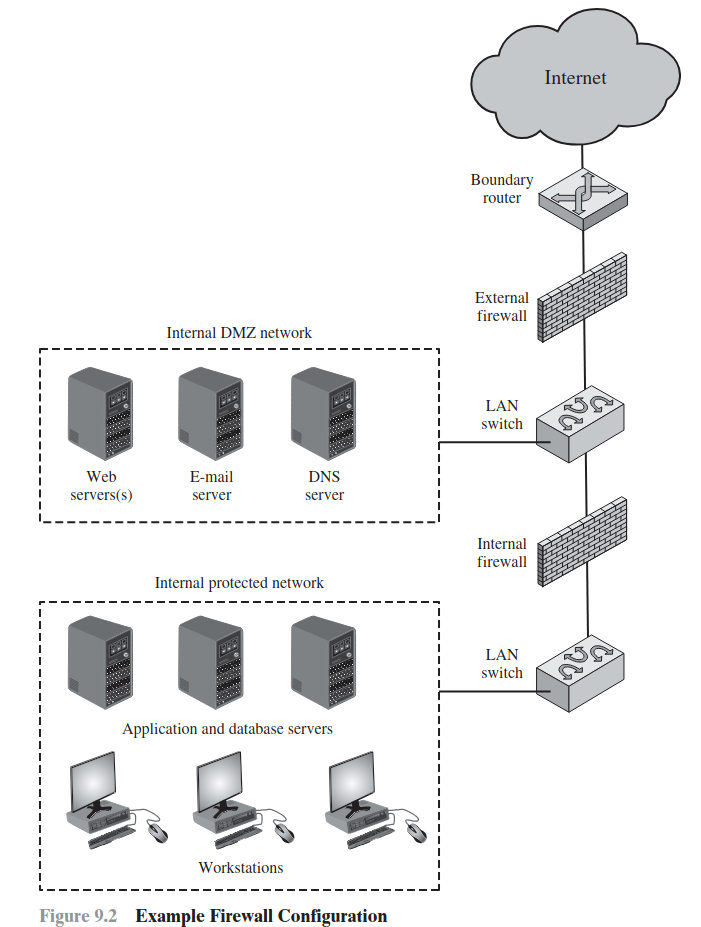
\includegraphics[width=0.4\textwidth]{Figuras/firewall-locations.png}


    \end{figure}

\end{frame}

\begin{frame}{Firewalls em dispositivos locais: Definição}
    \begin{itemize}
        \item \textbf{O que é?}
              \begin{itemize}
                  \item Controla o tráfego entre um \textbf{computador pessoal} (ou workstation) e a rede (Internet ou rede corporativa).
              \end{itemize}

        \item \textbf{Casos de Uso:}
              \begin{itemize}
                  \item Ambiente doméstico (home).
                  \item Intranets corporativas.
              \end{itemize}

        \item \textbf{Localização (Implementação):}
              \begin{itemize}
                  \item \textbf{1. Módulo de Software:} Tipicamente, roda no próprio computador pessoal.
                  \item \textbf{2. Roteador Doméstico:} Em ambientes com múltiplos computadores, a funcionalidade pode estar no roteador que se conecta ao modem (DSL/Cabo).
              \end{itemize}
    \end{itemize}
\end{frame}

\begin{frame}{Firewalls em dispositivos locais: Função e Implementações}
    \begin{itemize}
        \item \textbf{Complexidade:}
              \begin{itemize}
                  \item Tipicamente \textbf{muito menos complexos} que firewalls de servidor ou stand-alone.
              \end{itemize}

        \item \textbf{Função Principal (Defesa):}
              \begin{itemize}
                  \item Negar acesso remoto \textbf{não autorizado} ao computador.
              \end{itemize}

        \item \textbf{Função Secundária (Detecção):}
              \begin{itemize}
                  \item Monitorar atividade \textbf{de saída} (outgoing) na tentativa de detectar e bloquear malware (ex: worms).
              \end{itemize}

        \item \textbf{Implementações (Exemplos):}
              \begin{itemize}
                  \item Pacote \texttt{netfilter} (Linux).
                  \item Pacote \texttt{pf} (BSD e MacOS).
                  \item \texttt{Windows Firewall} (Windows).
              \end{itemize}

        \item \textbf{Configuração:}
              \begin{itemize}
                  \item Via linha de comando (CLI) ou interface gráfica (GUI).
              \end{itemize}
    \end{itemize}
\end{frame}

\begin{frame}{Firewalls em dispositivos locais: Política Padrão e Serviços}
    \begin{itemize}
        \item \textbf{Política Padrão (Default):}
              \begin{itemize}
                  \item \textbf{Conexões de Entrada (Inbound):} Geralmente \textbf{negadas}, exceto as que o usuário permite explicitamente.
                  \item \textbf{Conexões de Saída (Outbound):} Geralmente \textbf{permitidas}.
              \end{itemize}

        \item \textbf{Exemplos de serviços de entrada que podem ser reativados (portas):}
              \begin{columns}[T] % T = top aligned
                  \begin{column}{.5\textwidth}
                      \begin{itemize}
                          \item Personal file sharing (548, 427)
                          \item Windows sharing (139)
                          \item Personal Web sharing (80, 427)
                          \item Remote login—SSH (22)
                          \item FTP access (20-21, etc.)
                          \item Printer sharing (631, 515)
                          \item IChat Rendezvous (5297, 5298)
                          \item iTunes Music Sharing (3869)
                      \end{itemize}
                  \end{column}
                  \begin{column}{.5\textwidth}
                      \begin{itemize}
                          \item CVS (2401)
                          \item Gnutella/Limewire (6346)
                          \item ICQ (4000)
                          \item IRC (194)
                          \item MSN Messenger (6891-6900)
                          \item Network Time (123)
                          \item SMB (sem netbios–445)
                          \item VNC (5900-5902)
                      \end{itemize}
                  \end{column}
              \end{columns}
    \end{itemize}
\end{frame}

\begin{frame}{Firewalls em dispositivos locais: Regra de FTP e Recursos Avançados}
    \begin{itemize}
        \item \textbf{Exceção da Regra de FTP:}
              \begin{itemize}
                  \item Se o acesso FTP é habilitado, as portas 20 e 21 são abertas localmente.
                  \item Se \textit{outros} conectam \textit{a partir} das portas 20 ou 21, as portas 1024-65535 são abertas (para a conexão de dados do FTP).
              \end{itemize}

        \item \textbf{Recursos Avançados:}
              \begin{itemize}
                  \item \textbf{Stealth Mode:} "Esconde" o sistema na Internet ao \textbf{descartar (drop)} pacotes de comunicação não solicitados (fazendo parecer que o sistema não está presente).
                  \item \textbf{Bloqueio de UDP:} Restringe o tráfego (para portas abertas) apenas a pacotes TCP.
                  \item \textbf{Logging:} Ferramenta importante para verificar atividades indesejadas.
                  \item \textbf{Filtro de Aplicação:} Permite ao usuário especificar que \textbf{apenas aplicações selecionadas} (ou assinadas por uma CA válida) podem prover serviços na rede.
              \end{itemize}
    \end{itemize}
\end{frame}

\begin{frame}{9.5 Localização e Configurações do Firewall}
    \begin{itemize}
        \item O firewall é posicionado para prover uma \textbf{barreira protetora} entre uma fonte externa (potencialmente não confiável) e uma rede interna.

        \item O administrador de segurança deve decidir:
              \begin{itemize}
                  \item A \textbf{localização} do firewall.
                  \item O \textbf{número} de firewalls necessários.
              \end{itemize}

        \item Esta seção analisa algumas opções comuns de configuração e localização.
    \end{itemize}
\end{frame}

\begin{frame}{Configuração: Redes DMZ (Zona Desmilitarizada)}
    \begin{itemize}
        \item Uma configuração de firewall comum que inclui um \textbf{segmento de rede adicional} entre um firewall \textbf{externo} e um \textbf{interno}.

        \item \textbf{Firewall Externo:} Colocado na borda da rede (logo após o roteador de borda da Internet/WAN).

        \item \textbf{Firewall(s) Interno(s):} Protegem o grosso da rede corporativa (enterprise network).

        \item \textbf{A DMZ:} É a região (rede) localizada \textit{entre} esses dois firewalls.

        \item \textbf{Propósito da DMZ:}
              \begin{itemize}
                  \item Localizar sistemas que precisam ser \textbf{acessíveis externamente}, mas que ainda necessitam de \textbf{alguma proteção}.
                  \item \textbf{Exemplos de sistemas na DMZ:} Website corporativo, Servidor de e-mail (SMTP), Servidor DNS.
              \end{itemize}
    \end{itemize}
\end{frame}

\begin{frame}{DMZ: O Papel de Cada Firewall}
    \begin{itemize}
        \item \textbf{Função do Firewall Externo:}
              \begin{itemize}
                  \item Fornece controle de acesso e proteção (moderada) para os sistemas da DMZ (consistente com sua necessidade de conectividade).
                  \item Fornece um nível básico de proteção para o resto da rede interna.
              \end{itemize}

        \item \textbf{Três Propósitos do Firewall Interno:}
              \begin{enumerate}
                  \item \textbf{Filtragem mais rigorosa:} Adiciona capacidade de filtragem mais forte (comparado ao externo) para proteger os servidores/workstations internos de ataques externos.

                  \item \textbf{Proteção de Mão Dupla (vs. DMZ):}
                        \begin{itemize}
                            \item Protege a rede interna contra ataques lançados \textit{a partir} da DMZ (ex: se um servidor web for comprometido com malware, rootkits, bots).
                            \item Protege a DMZ contra ataques vindos da rede \textit{interna}.
                        \end{itemize}

                  \item \textbf{Segmentação Interna:}
                        \begin{itemize}
                            \item Múltiplos firewalls internos podem ser usados para proteger porções da rede interna umas das outras (ex: Servidores vs. Workstations, como na Fig 8.5).
                        \end{itemize}
              \end{enumerate}
    \end{itemize}
\end{frame}

\begin{frame}{Configuração: Redes Privadas Virtuais (VPNs)}
    \begin{itemize}
        \item \textbf{O Problema (Custo vs. Segurança):}
              \begin{itemize}
                  \item Organizações (com LANs em locais dispersos) precisam se interconectar.
                  \item Usar a \textbf{Internet} (rede pública) é mais barato e mais fácil de gerenciar (offloading) do que usar uma \textbf{rede privada} (linhas privadas).
                  \item \textbf{Mas:} A rede pública expõe o tráfego corporativo (eavesdropping, acesso não autorizado).
              \end{itemize}

        \item \textbf{A Solução (VPN):}
              \begin{itemize}
                  \item Um conjunto de computadores que se interconecta por uma rede insegura.
                  \item Usa \textbf{criptografia e autenticação} em camadas de protocolo inferiores.
                  \item Cria uma \textbf{conexão segura} através de uma rede insegura (Internet).
                  \item \textit{Pré-requisito:} Depende de ter o mesmo sistema de cripto/autenticação em ambas as pontas.
              \end{itemize}
    \end{itemize}
\end{frame}

\begin{frame}{VPNs: Implementação com IPsec}
    \begin{itemize}
        \item A criptografia pode ser feita pelo \textbf{software do firewall} ou por roteadores.
        \item Protocolo mais comum: \textbf{IPsec} (nível IP).

        \item \textbf{Cenário Típico:}
              \begin{itemize}
                  \item Protocolos IPsec operam em dispositivos de rede (roteador ou firewall) que conectam a LAN ao mundo externo.
                  \item O dispositivo IPsec \textbf{criptografa e comprime} todo o tráfego que \textit{sai} para a WAN.
                  \item O dispositivo IPsec \textbf{descriptografa e descomprime} todo o tráfego que \textit{vem} da WAN.
                  \item Esta operação é \textbf{transparente} para os servidores e workstations na LAN.
              \end{itemize}

        \item \textbf{Usuários Individuais (Remotos):}
              \begin{itemize}
                  \item Também podem usar IPsec, mas o \textit{próprio workstation} deve implementar os protocolos e ter alta segurança de host (tornando-se um alvo atraente).
              \end{itemize}
    \end{itemize}
\end{frame}

\begin{frame}{VPNs: Onde implementar o IPsec?}
    \begin{itemize}
        \item Um local lógico para implementar o IPsec é \textbf{no firewall}.

        \item \textbf{Problema 1: IPsec \textit{atrás} (interno) do firewall}
              \begin{itemize}
                  \item O tráfego VPN que passa pelo firewall (em ambas as direções) está \textbf{criptografado}.
                  \item \textbf{Consequência:} O firewall é \textbf{incapaz} de realizar suas funções (filtragem, scan de vírus, log, controle de acesso, etc.), pois não vê o tráfego em claro.
              \end{itemize}

        \item \textbf{Problema 2: IPsec \textit{no roteador de borda} (externo ao firewall)}
              \begin{itemize}
                  \item O dispositivo (roteador) é provavelmente \textbf{menos seguro} que o firewall.
                  \item Portanto, é uma plataforma menos desejável para o IPsec.
              \end{itemize}

        \item \textit{(Solução implícita: A implementação do IPsec no próprio firewall é a mais funcional).}
    \end{itemize}
\end{frame}

\begin{frame}{Configuração: Firewalls Distribuídos}
    \begin{itemize}
        \item \textbf{O que é?} Uma configuração que envolve:
              \begin{itemize}
                  \item Dispositivos de firewall stand-alone (de rede).
                  \item \textbf{E} Host-Based Firewalls (em servidores, workstations).
              \end{itemize}

        \item \textbf{Característica Chave:} Trabalham juntos sob um \textbf{controle administrativo central}.

        \item \textbf{Gerenciamento:}
              \begin{itemize}
                  \item Administradores configuram firewalls em centenas de servidores/workstations e firewalls pessoais (locais e remotos).
                  \item Ferramentas permitem ao admin definir políticas e monitorar a segurança em \textbf{toda a rede}.
              \end{itemize}

        \item \textbf{Vantagem:}
              \begin{itemize}
                  \item Proteção contra \textbf{ataques internos}.
                  \item Proteção \textbf{personalizada} (tailored) para máquinas e aplicações específicas.
              \end{itemize}
    \end{itemize}
\end{frame}

\begin{frame}{Configuração: Firewalls Distribuídos}
    \begin{itemize}
        \item \textbf{O que é?} Uma configuração que envolve:
              \begin{itemize}
                  \item Dispositivos de firewall stand-alone (de rede).
                  \item \textbf{E} Host-Based Firewalls (em servidores, workstations).
              \end{itemize}

        \item \textbf{Característica Chave:} Trabalham juntos sob um \textbf{controle administrativo central}.

        \item \textbf{Gerenciamento:}
              \begin{itemize}
                  \item Administradores configuram firewalls em centenas de servidores/workstations e firewalls pessoais (locais e remotos).
                  \item Ferramentas permitem ao admin definir políticas e monitorar a segurança em \textbf{toda a rede}.
              \end{itemize}

        \item \textbf{Vantagem:}
              \begin{itemize}
                  \item Proteção contra \textbf{ataques internos}.
                  \item Proteção \textbf{personalizada} (tailored) para máquinas e aplicações específicas.
              \end{itemize}
    \end{itemize}
\end{frame}
%\title{Aula 15 - IDS/IPS}

\author{Prof. Gabriel Rodrigues Caldas de Aquino}

\institute
{
    Instituto de Computação \\
    Universidade Federal do Rio de Janeiro\\
    gabrielaquino@ic.ufrj.br% Your institution for the title page
}
\date{Compilado em: \\ \today} % Date, can be changed to a custom date

%----------------------------------------------------------------------------------------
%    PRESENTATION SLIDE
%----------------------------------------------------------------------------------------



\begin{frame}
    % Print the title page as the first slide
    \titlepage
\end{frame}

\begin{frame}{A Ameaça: Intrusos e a Necessidade de Defesa}
    \begin{itemize}
        \item Uma das principais ameaças à segurança são os \textbf{intrusos}.



        \item Boa parte das violações são feitas por \textbf{outsiders}
        \item Mas existem algumas violações feitas por \textbf{insiders}.
        \item \textbf{Porém:} Insiders podem ser muito mais perigosos.


        \item \textbf{Preocupação:} Ataques \textbf{direcionados} a indivíduos e seus sistemas de TI.


        \item \textbf{Implicação:}
              \begin{itemize}
                  \item Ataques direcionados podem \textit{burlar} as defesas de perímetro (ex: Firewalls).
                  \item É necessário estratégias de \textbf{Defesa em Profundidade}.
              \end{itemize}
    \end{itemize}
\end{frame}

\begin{frame}{Classes de Intrusos (Parte 1): Ciber criminosos e Ativistas}
    Entender a \textbf{motivação} dos atacantes auxilia no design da estratégia defensiva.
    \begin{itemize}


        \item \textbf{Classe 1: Ciber criminosos}
              \begin{itemize}
                  \item \textbf{Motivação:} \textbf{Recompensa Financeira}.
                  \item \textbf{Atividades:} Roubo de identidade, roubo de credenciais financeiras, espionagem corporativa, roubo ou sequestro de dados.
                  \item \textbf{Perfil:} Organizam-se em fóruns \textit{underground} (ex: DarkMarket) para trocar dados e coordenar ataques.
              \end{itemize}

        \item \textbf{Classe 2: Ativistas}
              \begin{itemize}
                  \item \textbf{Motivação:} \textbf{Causas sociais ou políticas}.
                  \item \textbf{Nível de Habilidade:} Frequentemente baixo.
                  \item \textbf{Atividades:} Promover a causa através de \textit{website defacement}, DoS, ou vazamento de dados.
                  \item \textbf{Exemplos:} Anonymous, LulzSec, Manning, Snowden.
              \end{itemize}
    \end{itemize}
\end{frame}

\begin{frame}{Classes de Intrusos (Parte 2): APTs e Outros}
    \begin{itemize}
        \item \textbf{Classe 3: APTs}
              \begin{itemize}
                  \item \textbf{Quem são?} Grupos de hackers \textbf{patrocinados por governos}.
                  \item \textbf{Motivação:} Conduzir \textbf{espionagem} ou \textbf{sabotagem}.
                  \item \textbf{Alias:} \textbf{APTs (Advanced Persistent Threats)} – devido à natureza \textbf{secreta} e \textbf{persistência} por longos períodos.
                  \item \textbf{Escopo:} Generalizado (China, Rússia, EUA, UK, etc.).
              \end{itemize}

        \item \textbf{Classe 4: Outros}
              \begin{itemize}
                  \item \textbf{Hackers Clássicos:}
                        \begin{itemize}
                            \item \textbf{Motivação:} Desafio técnico, ou estima e reputação no grupo.
                            \item Ex: Responsáveis por descobrir novas vulnerabilidades, como buffer overflow.
                        \end{itemize}
                  \item \textbf{Hobby Hackers:}
                        \begin{itemize}
                            \item Usam \textit{attack toolkits} (ferramentas prontas) para explorar.
                            \item Potencialmente podem ser recrutados pelas outras classes.
                        \end{itemize}
              \end{itemize}
    \end{itemize}
\end{frame}

\begin{frame}{Exemplos de Intrusão (NIST SP 800-61) - Parte 1}

    O NIST SP 800-61 (Guia de Resposta a Incidentes) lista os seguintes exemplos de intrusão:
    \begin{itemize}

        \item Realizar um comprometimento \textit{root} remoto de um servidor de e-mail.

        \item Pichar (defacing) um servidor Web.

        \item Adivinhar e quebrar senhas.

        \item Copiar um banco de dados contendo números de cartão de crédito.

        \item Visualizar dados sensíveis (folha de pagamento, registros médicos) sem autorização.
    \end{itemize}
\end{frame}

\begin{frame}{Exemplos de Intrusão (NIST SP 800-61) - Parte 2}
    \begin{itemize}
        \item Executar um \textit{packet sniffer} em uma estação de trabalho para capturar nomes de usuário e senhas.

        \item Usar um erro de permissão em um servidor FTP anônimo para distribuir software pirata e arquivos de música.

        \item Acessar sistema inseguro e obter acesso à rede interna.

        \item \textbf{Engenharia Social}

    \end{itemize}
\end{frame}

\begin{frame}{O Papel e as Limitações do IDS/IPS}
    \begin{itemize}

        \item \textbf{IDS: Sistemas de Detecção de Intrusão}
        \item \textbf{IPS: Sistemas de Prevenção de Intrusão}


        \item \textbf{Onde funcionam bem:}
              \begin{itemize}
                  \item São razoavelmente eficazes contra ataques \textbf{conhecidos} e \textbf{menos sofisticados}.
                  \item Ex: Ataques de grupos ativistas ou golpes de e-mail em larga escala.
              \end{itemize}

        \item \textbf{Onde falham:}
              \begin{itemize}
                  \item São \textbf{menos eficazes} contra ataques sofisticados e direcionados (ex: cibercriminosos ou APTs patrocinados pelo Estado).
                  \item \textit{Por quê?} Esses atacantes usam \textbf{\textit{zero-day exploits}} e sabem como \textbf{obscurecer} suas atividades no sistema.
              \end{itemize}

        \item \textbf{Defesa em Profundidade}
              \begin{itemize}
                  \item O IDS/IPS precisa ser parte de uma estratégia de \textbf{Defesa em Profundidade}. Incluindo criptografia, trilhas de auditoria, autenticação forte e gerenciamento ativo de segurança.
              \end{itemize}
    \end{itemize}
\end{frame}

\begin{frame}{Comportamento do Intruso: Metodologia de Ataque}
    Padrões de comportamento dos intrusos mudam e constantemente

    \begin{itemize}
        \item \textbf{Porém existe} uma metodologia de ataque comum:
              \begin{itemize}
                  \item Phishing $\rightarrow$ Instalação de Malware $\rightarrow$ Roubo de Credenciais $\rightarrow$ Comprometimento.
              \end{itemize}
    \end{itemize}
    \textbf{Etapas:}

    \begin{itemize}


        \item \textbf{1. Aquisição de Alvo e Coleta de Informações}
              \begin{itemize}
                  \item Ossint - Open source intelligence
                  \item Usa informações publicamente disponíveis (técnicas ou não)
                  \item Uso de ferramentas de mapeamento de rede
                  \item \textbf{Objetivo}: Identificar e caracterizar os sistemas-alvo.
              \end{itemize}

        \item \textbf{2. Acesso Inicial}
              \begin{itemize}
                  \item Explorando uma vulnerabilidade de rede remota.
                  \item Explorando credenciais de autenticação fracas.
                  \item Instalando malware (via \textbf{engenharia social} ou \textbf{download direcionado}).
              \end{itemize}
    \end{itemize}
\end{frame}

\begin{frame}{Metodologia de Ataque (Continuação)}
    \begin{itemize}
        \item \textbf{3. Escalação de Privilégio}
              \begin{itemize}
                  \item Ações tomadas \textbf{dentro} do sistema \textbf{após o acesso inicial}.
                  \item Explora vulnerabilidades de acesso \textit{local}.
                  \item \textbf{Objetivo:} Aumentar os privilégios disponíveis para o atacante, permitindo que ele atinja seus objetivos no sistema-alvo.
              \end{itemize}

        \item \textbf{4. Coleta de Informações ou Exploração do Sistema}
              \begin{itemize}
                  \item Ações do atacante para acessar ou modificar informações/recursos no sistema.
                  \item Pode incluir mudar para outro sistema-alvo (\textbf{movimentação lateral}).
              \end{itemize}
    \end{itemize}
\end{frame}

\begin{frame}{Metodologia de Ataque (Finalização)}
    \begin{itemize}
        \item \textbf{5. Manutenção do Acesso}
              \begin{itemize}
                  \item Ações para permitir acesso contínuo (persistência) pelo atacante.
                  \item Instalação de \textbf{backdoors} ou outro software malicioso.
                  \item Adição de credenciais de autenticação "secretas" .
                  \item Outras mudanças de configuração no sistema.
              \end{itemize}

        \item \textbf{6. Apagando Rastros}
              \begin{itemize}
                  \item O atacante desabilita ou edita \textbf{logs de auditoria} para remover evidências da atividade de ataque.
                  \item Usa \textbf{rootkits} e outras medidas para esconder arquivos ou códigos instalados secretamente.
              \end{itemize}
    \end{itemize}
\end{frame}

\begin{frame}{Examplos de Comportamento do Intruso}
    \begin{itemize}
        \item \textbf{(a) Aquisição de Alvo e Coleta de Informações}
              \begin{itemize}
                  \item Explorar site corporativo (estrutura, pessoal, S.O.).
                  \item Usar DNS lookup (\texttt{dig}, \texttt{host}) e banco de dados \texttt{WHOIS}.
                  \item Mapear serviços de rede (\texttt{NMAP}).
                  \item Enviar e-mail de "sondagem" (ex: SAC) para analisar a resposta (tipo de cliente/servidor de e-mail).
                  \item Identificar serviços vulneráveis (ex: um CMS Web).
              \end{itemize}

        \item \textbf{(b) Acesso Inicial}
              \begin{itemize}
                  \item \textit{Brute force} (adivinhação) de senha (ex: do CMS).
                  \item Explorar uma vulnerabilidade em um plugin (ex: do CMS) para ganhar acesso ao sistema.
                  \item Enviar e-mail de \textit{spear-phishing} direcionado (com link para um \textit{exploit} de navegador).
              \end{itemize}
    \end{itemize}
\end{frame}
\begin{frame}{Examplos de Comportamento do Intruso}
    \begin{itemize}
        \item \textbf{(c) Escalação de Privilégio (Privilege Escalation)}
              \begin{itemize}
                  \item Escanear o sistema por aplicações com \textit{exploits} locais.
                  \item Explorar uma aplicação vulnerável para ganhar privilégios elevados (ex: root/admin).
                  \item Instalar \textit{sniffers} para capturar senhas de administrador na rede.
                  \item Usar a senha de admin capturada para acessar informação privilegiada.
              \end{itemize}

        \item \textbf{(d) Coleta de Informações ou Exploração do Sistema}
              \begin{itemize}
                  \item Escanear arquivos em busca da informação desejada (ex: dados financeiros, PII).
                  \item Transferir um grande número de documentos para um repositório externo (exfiltração de dados).
                  \item Usar senhas (capturadas) para acessar outros servidores na rede (movimentação lateral).
              \end{itemize}
    \end{itemize}
\end{frame}
\begin{frame}{Examplos de Comportamento do Intruso}
    \begin{itemize}
        \item \textbf{(e) Manutenção de Acesso }
              \begin{itemize}
                  \item Instalar uma ferramenta de administração remota (RAT) ou \textit{rootkit} com um \textit{backdoor} para acesso futuro.
                  \item Usar a senha de administrador (capturada) para acessar a rede posteriormente (persistência).
                  \item Modificar ou desabilitar programas de antivírus (AV) ou IDS rodando no sistema para evitar detecção.
              \end{itemize}

        \item \textbf{(f) Apagando Rastros }
              \begin{itemize}
                  \item Usar um \textit{rootkit} para esconder os arquivos (ex: RAT, sniffers) instalados no sistema.
                  \item Editar arquivos de log (\textit{logfiles}) para remover as entradas (evidências) geradas durante a intrusão.
              \end{itemize}
    \end{itemize}
\end{frame}

\begin{frame}{Detecção de Intrusão (Intrusion Detection): Definições}
    \begin{itemize}
        \item \textbf{Intrusão de Segurança:}
              \begin{itemize}
                  \item Um ato \textbf{não autorizado} de \textbf{burlar (bypassing)} os mecanismos de segurança de um sistema.
              \end{itemize}

        \item \textbf{Detecção de Intrusão :}
              \begin{itemize}
                  \item Uma função de hardware ou software que \textbf{coleta e analisa} informações de várias áreas (dentro de um computador ou rede).
                  \item \textbf{Objetivo:} Identificar possíveis intrusões de segurança.
              \end{itemize}
    \end{itemize}
\end{frame}

\begin{frame}{Componentes Lógicos de um IDS}
    \begin{itemize}
        \item Um IDS (Intrusion Detection System) é composto por três componentes lógicos:

        \item \textbf{1. Sensores }
              \begin{itemize}
                  \item Responsáveis por \textbf{coletar dados}.
                  \item A entrada pode ser qualquer parte do sistema que contenha evidência de intrusão
                  \item Ex: pacotes de rede, arquivos de log, system calls.
                  \item Os sensores coletam e encaminham esta informação para o Analisador.
              \end{itemize}

        \item \textbf{2. Analisadores }
              \begin{itemize}
                  \item Recebem a entrada de um ou mais Sensores.
                  \item A saída \textbf{determina se uma intrusão ocorreu}.
                  \item Pode incluir evidências e orientações sobre ações.
                  \item Os dados dos sensores também podem ser armazenados para análise futura.
              \end{itemize}

        \item \textbf{3. Interface de Usuário }
              \begin{itemize}
                  \item Permite ao administrador \textbf{visualizar} o sistema ou \textbf{controlar o seu comportamento}.

              \end{itemize}
    \end{itemize}
\end{frame}

\begin{frame}{Classificação de IDSs (Baseado na Fonte de Dados)}
    \textbf{Arquitetura:}


    \begin{itemize}
        \item \textbf{Simples:} Um IDS com um único sensor e analisador - Ex:  um HIDS ou  NIDS.
        \item \textbf{Distribuída:} Uso de \textbf{múltiplos sensores} em vários hosts e dispositivos de rede, enviando informações para um \textbf{analisador centralizado}.
    \end{itemize}

    \textbf{Classificação (Fonte e Tipo de Dados):}
    \begin{itemize}
        \item \textbf{1. Host-based IDS (HIDS)}
              \begin{itemize}
                  \item \textbf{O que monitora?} As características de um \textbf{único host} e os eventos ocorrendo nele.
                  \item \textit{Exemplos:} Identificadores de processo (PIDs), \textit{system calls} (chamadas de sistema).
              \end{itemize}

        \item \textbf{2. Network-based IDS (NIDS)}
              \begin{itemize}
                  \item \textbf{O que monitora?} O \textbf{tráfego de rede} de segmentos ou dispositivos específicos.
                  \item \textit{Exemplos:} Analisa tráfego da rede para identificar atividades suspeitas.
              \end{itemize}

        \item \textbf{3. Distributed ou Hybrid IDS (Distribuído/Híbrido)}
              \begin{itemize}
                  \item \textbf{O que faz?} Combina informações de vários sensores (HIDS e/ou NIDS) em um analisador central.
                  \item \textit{Vantagem:} Consegue identificar e responder melhor à atividade de intrusão.
              \end{itemize}
    \end{itemize}
\end{frame}

\begin{frame}{Princípios Básicos: Motivações para o IDS}
    \begin{itemize}
        \item Autenticação, Controle de Acesso e Firewalls ajudam a combater intrusões.
        \item A \textbf{Detecção de Intrusão (IDS)} é outra linha de defesa, motivada por várias considerações:

        \item \textbf{1. Detecção Rápida }
              \begin{itemize}
                  \item Se a intrusão for detectada rápido o suficiente, o intruso pode ser \textbf{ejetado} do sistema \textit{antes} de causar danos ou comprometer dados.
                  \item Mesmo se não for a tempo de "preempt" (impedir), quanto mais cedo a detecção, menor o dano e mais rápida a recuperação.
              \end{itemize}

        \item \textbf{2. Efeito desencorajador}
              \begin{itemize}
                  \item Um IDS eficaz pode desencorajar ataques, atuando assim para \textbf{prevenir} intrusões.
              \end{itemize}

        \item \textbf{3. Coleta de Informações}
              \begin{itemize}
                  \item A detecção permite a coleta de informações sobre \textbf{técnicas de intrusão}.
                  \item Essas informações podem ser usadas para fortalecer as medidas de \textbf{prevenção} (ex: regras de firewall, patches).
              \end{itemize}
    \end{itemize}
\end{frame}

\begin{frame}{Princípios Básicos: A Suposição Fundamental do IDS}
    \begin{itemize}
        \item \textbf{A Suposição:}
              \begin{itemize}
                  \item A detecção de intrusão baseia-se na suposição de que o comportamento do \textbf{intruso} difere do comportamento de um \textbf{usuário legítimo} de maneiras que podem ser \textbf{quantificadas}.
              \end{itemize}

        \item \textbf{O Desafio (A Realidade):}
              \begin{itemize}
                  \item Não podemos esperar que haja uma distinção \textbf{nítida (crisp) e exata} entre um ataque e o uso normal dos recursos.
              \end{itemize}

        \item \textbf{A Consequência (Falsos Positivos/Negativos):}
              \begin{itemize}
                  \item Devemos esperar que haverá alguma \textbf{sobreposição (overlap)} entre o comportamento legítimo e o comportamento de ataque.
                  \item (O trabalho do Analisador é minimizar essa sobreposição).
              \end{itemize}
    \end{itemize}
\end{frame}

\begin{frame}{O Desafio Central do IDS: O "Trade-Off"}
    \begin{itemize}
        \item O comportamento típico de um intruso e de um usuário autorizado não são perfeitamente distintos; existe uma \textbf{sobreposição (overlap)}.

        \item \textbf{O Dilema (Compromisso):}
              \begin{itemize}
                  \item \textbf{1. Interpretação "Frouxa" (Loose):}
                        \begin{itemize}
                            \item Tenta capturar o máximo de intrusos.
                            \item \textbf{Resultado:} Leva a um alto número de \textbf{Falsos Positivos} (Falsos Alarmes), onde usuários autorizados são identificados como intrusos.
                        \end{itemize}
                  \item \textbf{2. Interpretação "Restrita" (Tight):}
                        \begin{itemize}
                            \item Tenta limitar os Falsos Positivos.
                            \item \textbf{Resultado:} Leva a um aumento de \textbf{Falsos Negativos} (intrusos não identificados).
                        \end{itemize}
              \end{itemize}

        \item \textbf{O Objetivo Ideal:}
              \begin{itemize}
                  \item A prática do IDS é um "compromisso" (e uma "arte").
                  \item Maximizar a \textbf{Taxa de Detecção} (detectar ataques reais).
                  \item Minimizar a \textbf{Taxa de Falsos Alarmes} (ignorar uso normal).
              \end{itemize}
    \end{itemize}
\end{frame}

\begin{frame}{A Visão Clássica}

    A dificuldade de detecção depende do tipo de intruso:
    \begin{itemize}


        \item \textbf{Detectando Atacantes Externos (Outsiders):}
              \begin{itemize}
                  \item É possível (com confiança razoável) distinguir um atacante externo de um usuário legítimo.
                  \item \textbf{Como?} Padrões de comportamento legítimo podem ser estabelecidos (observando o histórico).
                  \item \textbf{Detecção:} Pode-se detectar \textbf{desvios significativos} (anomalias) desses padrões.
              \end{itemize}

        \item \textbf{Detectando Atacantes Internos (Insiders):}
              \begin{itemize}
                  \item (Um usuário legítimo agindo de forma não autorizada).
                  \item Anderson concluiu que esta é a tarefa \textbf{mais difícil}.
                  \item \textbf{Por quê?} A distinção entre o comportamento "anormal" (malicioso) e "normal" (legítimo) de um insider pode ser \textbf{muito pequena}.
                  \item \textbf{Conclusão:} A busca \textit{apenas} por anomalias seria \textbf{insuficiente} para detectar insiders.
                  \item \textbf{Solução (sugerida):} O comportamento do insider pode ser detectável através de uma \textbf{definição inteligente} de condições (regras) que sugerem uso não autorizado.
              \end{itemize}
    \end{itemize}
\end{frame}

\begin{frame}{O Desafio Prático do IDS}
    \begin{itemize}
        \item \textbf{O Objetivo Duplo (e Conflitante):}
              \begin{itemize}
                  \item \textbf{1. Alta Taxa de Detecção:} Detectar uma porcentagem substancial de intrusões (senão, o IDS gera uma \textit{falsa sensação de segurança}).
                  \item \textbf{2. Baixa Taxa de Falsos Alarmes:} Se os falsos positivos (alarmes) forem frequentes, os gerentes \textbf{passarão a ignorar os alarmes} ou perderão muito tempo analisando-os.
              \end{itemize}

        \item \textbf{A Falácia da Taxa-Base (Base-Rate Fallacy):}
              \begin{itemize}
                  \item É \textbf{extremamente difícil} atingir os dois objetivos.
                  \item \textbf{O Problema:} O número real de \textbf{intrusões} (taxa-base) é \textbf{muito baixo} em comparação com o número de \textbf{usos legítimos} (normal).
                  \item \textbf{A Consequência:} A menos que o teste (o IDS) seja \textit{extremamente discriminatório} (quase perfeito), a taxa de falsos alarmes será \textbf{alta}.
                  \item \textbf{O desafio está aqui}
              \end{itemize}
    \end{itemize}
\end{frame}

\begin{frame}{Requisitos de um IDS - Parte 1}

    Um IDS deve:
    \begin{itemize}


        \item \textbf{1. Rodar continuamente} com mínima supervisão humana.

        \item \textbf{2. Ser tolerante a falhas}, ou seja, capaz de se recuperar de \textit{crashes} e reinicializações.

        \item \textbf{3. Resistir à subversão.} O IDS deve ser capaz de monitorar a si mesmo e detectar se foi modificado por um atacante.

        \item \textbf{4. Impor um \textit{overhead} mínimo} no sistema onde está rodando.

        \item \textbf{5. Ser configurável} de acordo com as políticas de segurança do sistema que está sendo monitorado.
    \end{itemize}
\end{frame}

\begin{frame}{Requisitos de um IDS - Parte 2}sobrecarga
    \begin{itemize}
        \item \textbf{6. Ser capaz de se adaptar} a mudanças no comportamento do sistema e dos usuários ao longo do tempo.

        \item \textbf{7. Ser capaz de escalar } para monitorar um grande número de hosts.

        \item \textbf{8. Evitar parada completa} do serviço, ou seja, se alguns componentes pararem, o resto deve ser afetado o mínimo possível.

        \item \textbf{9. Permitir reconfiguração dinâmica}, ou seja, a capacidade de reconfigurar o IDS sem ter que reiniciá-lo.
    \end{itemize}
\end{frame}

\begin{frame}{Abordagens de Análise de um IDS}
    Os IDSs usam duas abordagens:
    \begin{itemize}


        \item \textbf{1. Detecção de Anomalia}


        \item \textbf{2. Detecção por Assinatura ou Heurística }

    \end{itemize}
\end{frame}



\begin{frame}{Abordagens de Análise de um IDS}

    \begin{itemize}


        \item \textbf{1. Detecção de Anomalia}
              \begin{itemize}
                  \item \textbf{Como funciona?} Envolve a coleta de dados sobre o comportamento de \textbf{usuários legítimos} ao longo do tempo (criando uma "linha de base" do que é \textbf{normal}).
                  \item \textbf{Análise:} O comportamento \textit{atual} observado é então analisado.
                  \item \textbf{Decisão:} O IDS determina se o comportamento atual é de um usuário legítimo ou se é uma \textbf{anomalia} desse padrão, indicando um intruso.
              \end{itemize}


    \end{itemize}
\end{frame}




\begin{frame}{Abordagem de Análise: Detecção de Anomalia (Definição)}
    Duas fases:
    \begin{itemize}

        \item \textbf{1. Fase de Treinamento}
              \begin{itemize}
                  \item Desenvolve um \textbf{modelo} do comportamento legítimo (normal) do usuário.
                  \item Como? Coletando e processando dados dos sensores durante a operação normal do sistema.
                  \item (Pode ocorrer em momentos distintos ou ser um processo contínuo de evolução do modelo).
              \end{itemize}

        \item \textbf{2. Fase de Detecção}
              \begin{itemize}
                  \item O comportamento \textbf{atual} observado é comparado com o modelo (normal).
                  \item O comportamento é então classificado como \textbf{legítimo} ou \textbf{anômalo} (suspeito).
              \end{itemize}
    \end{itemize}
\end{frame}

\begin{frame}{Detecção de Anomalia: Categorias de Classificação}
    Temos três abordagens:
    \begin{itemize}


        \item \textbf{1. Estatística}
              \begin{itemize}
                  \item Análise do comportamento observado usando modelos (univariados, multivariados, time-series) das métricas.
              \end{itemize}

        \item \textbf{2. Baseada em Conhecimento}
              \begin{itemize}
                  \item Usa um \textbf{sistema especialista} (expert system) que classifica o comportamento de acordo com um conjunto de \textbf{regras} que modelam o comportamento legítimo.
              \end{itemize}

        \item \textbf{3. Aprendizado de Máquina (Machine-learning)}
              \begin{itemize}
                  \item Determina \textbf{automaticamente} um modelo de classificação adequado a partir dos dados de treinamento, usando técnicas de mineração de dados.
              \end{itemize}


    \end{itemize}
\end{frame}

\begin{frame}{Abordagem 1: Estatística}
    Desenvolve um \textbf{perfil estatístico} das métricas observadas.
    \begin{itemize}
        \item \textbf{Uso de:}
              \begin{itemize}
                  \item \textit{Univariada:} Trata cada métrica como independente (muito "cru" (crude), ineficaz).
                  \item \textit{Multivariada:} Considera correlações entre métricas (melhor discriminação).
                  \item \textit{Séries Temporais (Time-series):} Usa a ordem e o tempo entre eventos (ainda melhor).
              \end{itemize}

        \item \textbf{Vantagens:}
              \begin{itemize}
                  \item Relativa simplicidade e baixo custo computacional.
                  \item Não necessita de suposições (assumptions) sobre o comportamento esperado.
              \end{itemize}

        \item \textbf{Desvantagens:}
              \begin{itemize}
                  \item Dificuldade em selecionar métricas adequadas (balanço de falsos positivos/negativos).
                  \item Nem todos os comportamentos podem ser modelados por esta abordagem.
              \end{itemize}
    \end{itemize}
\end{frame}

\begin{frame}{Abordagem 2: Baseada em Conhecimento}
    \begin{itemize}
        \item Classifica os dados observados usando um \textbf{conjunto de regras} (expert system).

        \item \textbf{Fase de Treinamento:}
              \begin{itemize}
                  \item As regras são desenvolvidas (podendo ser \textbf{manualmente}) para caracterizar os dados de treinamento em classes distintas.
                  \item Pode usar ferramentas formais: máquinas de estado finito, linguagens de descrição.
              \end{itemize}

        \item \textbf{Vantagens:}
              \begin{itemize}
                  \item Robustez e flexibilidade.
              \end{itemize}

        \item \textbf{Desvantagens:}
              \begin{itemize}
                  \item \textbf{Dificuldade e tempo} para desenvolver regras (conhecimento) de alta qualidade.
                  \item Necessidade de \textbf{especialistas humanos} (human experts) para auxiliar no processo.
              \end{itemize}
    \end{itemize}
\end{frame}

\begin{frame}{Abordagem 3: Aprendizado de Máquina (Conceito e Trade-offs)}
    \begin{itemize}
        \item Usa técnicas de \textit{data mining} para desenvolver \textbf{automaticamente} um modelo a partir dos dados de treinamento (normais).

        \item \textbf{Fase de Treinamento (Custo):}
              \begin{itemize}
                  \item Requer \textbf{tempo significativo} e \textbf{altos recursos computacionais}.
              \end{itemize}

        \item \textbf{Fase de Detecção (Eficiência):}
              \begin{itemize}
                  \item Uma vez que o modelo é gerado, a análise subsequente (classificação) é geralmente \textbf{bastante eficiente}.
              \end{itemize}

        \item \textbf{Vantagens:}
              \begin{itemize}
                  \item Flexibilidade e adaptabilidade.
                  \item Capacidade de capturar interdependências complexas entre as métricas.
              \end{itemize}

        \item \textbf{Desvantagens:}
              \begin{itemize}
                  \item Dependência de suposições sobre o comportamento "aceito".
                  \item Taxa de \textbf{falsos alarmes} (false alarm rate) \textbf{inaceitavelmente alta} (atualmente).
                  \item Alto custo de recursos (para treinar).
              \end{itemize}
    \end{itemize}
\end{frame}

\begin{frame}{Abordagem 3: Aprendizado de Máquina - Abordagens}
    Várias abordagens de ML foram tentadas com sucesso variado:

    \begin{itemize}

        \item \textbf{Redes Bayesianas:} Codifica relações probabilísticas.

        \item \textbf{Modelos de Markov:} Modelo com conjuntos de estados interligados por probabilidades de transição.

        \item \textbf{Redes Neurais:} Para classificar dados.

        \item \textbf{Lógica Fuzzy:} Raciocínio é aproximado; pode acomodar incerteza.

        \item \textbf{Algoritmos Genéticos:} Desenvolver regras de classificação.

        \item \textbf{Clusterização e Detecção de Outlier:} Agrupa dados por similaridade; novos dados são classificados como "dentro de um cluster" (normal) ou "outlier" (anomalia).
    \end{itemize}
\end{frame}

\begin{frame}{Abordagens de Análise de um IDS}

    \begin{itemize}




        \item \textbf{2. Detecção por Assinatura ou Heurística }
              \begin{itemize}
                  \item Também conhecida como \textbf{Detecção de Mau Uso }.
                  \item \textbf{Como funciona?} Usa um conjunto de \textbf{padrões maliciosos conhecidos} ou \textbf{regras de ataque}.
                  \item \textbf{Análise:} O comportamento atual é comparado com este conjunto de regras/assinaturas.
                  \item \textbf{Decisão:} Se houver uma correspondência, é considerado um intruso.
              \end{itemize}
    \end{itemize}
\end{frame}


\begin{frame}{Abordagem de Análise: Detecção por Assinatura }
    \begin{itemize}

        \item \textbf{Como Funciona:}
              \begin{itemize}
                  \item Compara os dados coletados com \textbf{padrões conhecidos de dados maliciosos}.
                  \item As assinaturas precisam dar detalhes o suficiente para minimizar falsos alarmes, mas ainda detectar uma fração suficiente de dados maliciosos.
              \end{itemize}

        \item \textbf{Onde é usado:} Amplamente utilizado em produtos antivírus, proxies de varredura de tráfego de rede e NIDS.

        \item \textbf{Vantagens:}
              \begin{itemize}
                  \item Custo relativamente baixo em tempo e uso de recursos.
                  \item Ampla aceitação.
              \end{itemize}

        \item \textbf{Desvantagens:}
              \begin{itemize}
                  \item Esforço significativo necessário para identificar e revisar novos comportamentos para criar assinaturas.
                  \item \textbf{Incapacidade de detectar ataques "zero-day"} onde nenhuma assinatura existe.
              \end{itemize}
    \end{itemize}
\end{frame}

\begin{frame}{Abordagem de Análise: Detecção Heurística}
    \begin{itemize}
        \item \textbf{Como Funciona:}
              \begin{itemize}
                  \item Envolve o uso de \textbf{regras} para identificar ataques \textbf{conhecidos} ou que explorariam \textbf{fraquezas conhecidas}.

                  \item As regras também podem identificar comportamento \textbf{suspeito}, mesmo que esse comportamento esteja dentro dos padrões de uso estabelecidos.
              \end{itemize}

        \item \textbf{Desenvolvimento das Regras:}
              \begin{itemize}
                  \item Abordagem mais frutífera: \textbf{Analisar ferramentas e scripts de ataque} coletados na Internet.
                  \item Suplementado por regras geradas por \textbf{especialistas}.
                  \item As regras são tipicamente específicas para a máquina e o S.O.
              \end{itemize}

        \item \textbf{Exemplo:}
              \begin{itemize}
                  \item O sistema \textbf{SNORT} é um exemplo de um \textbf{NIDS baseado em regras}.
                  \item Existe uma grande coleção de regras para ele detectar uma ampla variedade de ataques de rede.
              \end{itemize}
    \end{itemize}
\end{frame}

\begin{frame}{Host-Based IDS (HIDS): Introdução}
    \begin{itemize}
        \item \textbf{O que é?}
              \begin{itemize}
                  \item O HIDS adiciona uma \textbf{camada especializada de software de segurança} a sistemas vulneráveis ou sensíveis.
                  \item \textit{Exemplos:} Servidores de banco de dados, sistemas administrativos.
              \end{itemize}

        \item \textbf{Função:}
              \begin{itemize}
                  \item Monitora a atividade \textbf{dentro do sistema} de várias maneiras para detectar comportamento suspeito.
              \end{itemize}

        \item \textbf{Propósito Principal:}
              \begin{itemize}
                  \item 1. Detectar intrusões.
                  \item 2. Registrar (log) eventos suspeitos.
                  \item 3. Enviar alertas.
                  \item IDS/IPS
              \end{itemize}


        \item \textbf{Abordagens de Análise:}
              \begin{itemize}
                  \item HIDS usa as duas abordagens:
                  \item Detecção de Anomalia (Anomaly).
                  \item Detecção por Assinatura ou Heurística.
              \end{itemize}
    \end{itemize}
\end{frame}

\begin{frame}{HIDS: Fontes de Dados e Sensores (Parte 1)}
    \begin{itemize}
        \item Um componente fundamental do IDS é o \textbf{sensor} que coleta dados. Um registro da atividade (input) deve ser fornecido ao analisador.
        \item Fontes de dados comuns incluem:

        \item \textbf{1. Rastros de Chamadas de Sistema }
              \begin{itemize}
                  \item Um registro da sequência de \textit{system calls} feitas pelos processos.
                  \item Amplamente reconhecida como a \textbf{fonte de dados preferida} para HIDS.
                  \item \textbf{Vantagem:} Funciona bem em sistemas Unix e Linux.
                  \item \textbf{Desvantagem:} Problemático em sistemas Windows (devido ao uso extensivo de DLLs, que "obscurecem" quais processos usam quais chamadas).
              \end{itemize}

        \item \textbf{2. Registros de Auditoria }
              \begin{itemize}
                  \item A maioria dos S.O. modernos inclui software de "accounting" (auditoria) que coleta informações sobre a atividade do usuário.
                  \item \textbf{Vantagem:} Nenhum software de coleta adicional é necessário.
                  \item \textbf{Desvantagem (1):} Os registros podem não conter a informação necessária ou não estar em um formato conveniente.
                  \item \textbf{Desvantagem (2):} Intrusos podem tentar \textbf{manipular} esses logs para esconder suas ações.
              \end{itemize}
    \end{itemize}
\end{frame}

\begin{frame}{HIDS: Fontes de Dados e Sensores (Parte 2)}
    \begin{itemize}
        \item \textbf{3. Checksums de Integridade de Arquivos }
              \begin{itemize}
                  \item Abordagem comum: Escanear periodicamente \textbf{arquivos críticos} (ex: arquivos de sistema) em busca de mudanças.
                  \item \textbf{Como?} Comparando hash atuais com um registro de valores conhecidos (baseline).
                  \item \textbf{Desvantagem (1):} A necessidade de gerar e proteger os checksums "bons" (baseline).
                  \item \textbf{Desvantagem (2):} A dificuldade de monitorar arquivos que \textit{mudam} (legitimamente) o tempo todo.
              \end{itemize}

        \item \textbf{4. Acesso ao Registro}
              \begin{itemize}
                  \item Uma abordagem usada em sistemas \textbf{Windows}.
                  \item Monitora o acesso ao Registro (dada a quantidade de informação e acesso usados pelos programas).
                  \item \textbf{Desvantagem:} Muito específico do Windows; registrou sucesso limitado.
              \end{itemize}

        \item \textbf{Função Resumida do Sensor:}
              \begin{itemize}
                  \item Coleta dados $\rightarrow$ Filtra (padroniza formato) $\rightarrow$ Encaminha para o Analisador.
              \end{itemize}
    \end{itemize}
\end{frame}

\begin{frame}{HIDS por Anomalia (Sistemas Linux/UNIX)}
    \begin{itemize}
        \item A maioria dos trabalhos em HIDS por anomalia foi feita em UNIX/Linux (dada a facilidade de coletar dados).

        \item \textbf{Fonte de Dados Preferida:} \textbf{Rastros de Chamadas de Sistema} .
              \begin{itemize}
                  \item Logs de auditoria.
              \end{itemize}

        \item \textbf{Por que "System Calls"?}
              \begin{itemize}
                  \item São o meio pelo qual os programas acessam as funções do \textbf{kernel}.
                  \item Fornecem informação \textbf{detalhada} sobre a atividade do processo, permitindo classificar como normal ou anômalo.
              \end{itemize}

    \end{itemize}
\end{frame}

\begin{frame}{HIDS (Linux) - Motores de Decisão }
    \begin{itemize}
        \item Os \textit{system call traces} (coletados) são analisados por um motor de decisão.

        \item \textbf{Abordagem Original (STIDE):}
              \begin{itemize}

                  \item Compara sequências de chamadas observadas com sequências "normais" (do treinamento) para obter uma "taxa de disparidade" (mismatch ratio).
              \end{itemize}

        \item \textbf{Abordagens Alternativas (ML):}
              \begin{itemize}
                  \item Hidden Markov Models (HMM)
                  \item Redes Neurais Artificiais (ANN)
                  \item Support Vector Machines (SVM)
                  \item Extreme Learning Machines (ELM)
              \end{itemize}

        \item \textbf{Performance:}
              \begin{itemize}
                  \item taxa\% detecção, falsos positivos.
                  \item velocidade de detecção.
              \end{itemize}
    \end{itemize}
\end{frame}

\begin{frame}{HIDS: Detecção por Assinatura ou Heurística}
    \begin{itemize}


        \item \textbf{Implementação Comum:} É a base dos \textbf{Antivírus}.
              \begin{itemize}
                  \item Usado em: sistemas cliente (PCs), dispositivos móveis, e incorporado em proxies (e-mail, Web) e NIDS.
              \end{itemize}

        \item \textbf{Como Funciona (Duas Técnicas):}
              \begin{itemize}
                  \item \textbf{1. Assinaturas :}
                        \begin{itemize}
                            \item Um banco de dados de \textbf{padrões de dados} (file signatures) encontrados em malware \textbf{conhecido}.
                        \end{itemize}
                  \item \textbf{2. Heurísticas:}
                        \begin{itemize}
                            \item Um conjunto de \textbf{regras} que caracterizam o \textbf{comportamento} malicioso \textbf{conhecido}.
                        \end{itemize}
              \end{itemize}

        \item \textbf{Vantagem:}
              \begin{itemize}
                  \item \textit{Muito eficiente} para detectar malware \textbf{conhecido}.
              \end{itemize}

        \item \textbf{Desvantagem :}
              \begin{itemize}
                  \item \textbf{NÃO é capaz} de detectar ataques \textbf{"zero-day"} (ataques novos/desconhecidos).
                  \item Pois o novo ataque não corresponde a nenhuma assinatura ou regra conhecida.
              \end{itemize}

        \item \textbf{Uso Principal:}
              \begin{itemize}
                  \item Amplamente utilizado, especialmente em sistemas \textbf{Windows} (que continuam a ser um alvo principal de intrusos).
              \end{itemize}
    \end{itemize}
\end{frame}

\begin{frame}{HIDS Distribuído}
    \begin{itemize}
        \item \textbf{O Foco Tradicional:}
              \begin{itemize}
                  \item O trabalho em HIDS (Host-based) focava-se na operação \textbf{\textit{stand-alone}} (em um único sistema).
              \end{itemize}

        \item \textbf{A Realidade Organizacional:}
              \begin{itemize}
                  \item A organização típica precisa defender uma coleção \textbf{distribuída} de hosts (suportados por uma LAN ou inter-rede).
              \end{itemize}

        \item \textbf{A Evolução (A Defesa Eficaz):}
              \begin{itemize}
                  \item Embora seja possível usar HIDS \textit{stand-alone} em cada host...
                  \item Uma defesa \textbf{mais eficaz} é alcançada através da \textbf{coordenação e cooperação} entre os IDSs pela rede (ou seja, um HIDS Distribuído).
              \end{itemize}
    \end{itemize}
\end{frame}

\begin{frame}{Network-Based IDS (NIDS): Definição e Papel}
    \begin{itemize}
        \item \textbf{O que é um NIDS?}
              \begin{itemize}
                  \item Monitora o tráfego em \textbf{pontos selecionados} de uma rede.
                  \item Examina o tráfego \textbf{pacote a pacote} em tempo real (ou próximo a isso).
                  \item Analisa atividade nos protocolos de Rede (L3), Transporte (L4) e/ou Aplicação (L7).
              \end{itemize}

        \item \textbf{Contraste (NIDS vs. HIDS):}
              \begin{itemize}
                  \item \textbf{NIDS:} Examina o \textit{tráfego de pacotes} \textbf{direcionado aos} sistemas.
                  \item \textbf{HIDS:} Examina a \textit{atividade do usuário e do software} \textbf{dentro de} um host.
              \end{itemize}

        \item \textbf{Papel e Localização:}
              \begin{itemize}
                  \item Tipicamente incluído na infraestrutura de \textbf{segurança de perímetro} (incorporado ou associado ao firewall).
                  \item Foco: Monitorar tentativas de intrusão \textbf{externa}.
              \end{itemize}

        \item \textbf{Arquitetura Típica:}
              \begin{itemize}
                  \item Sensores (para monitorar tráfego).
                  \item Servidores de Gerenciamento (para análise).
                  \item Consoles de Gerenciamento (para interface humana).
              \end{itemize}
    \end{itemize}
\end{frame}

\begin{frame}{Funcionamento NIDS}


    \begin{figure}
        \centering
        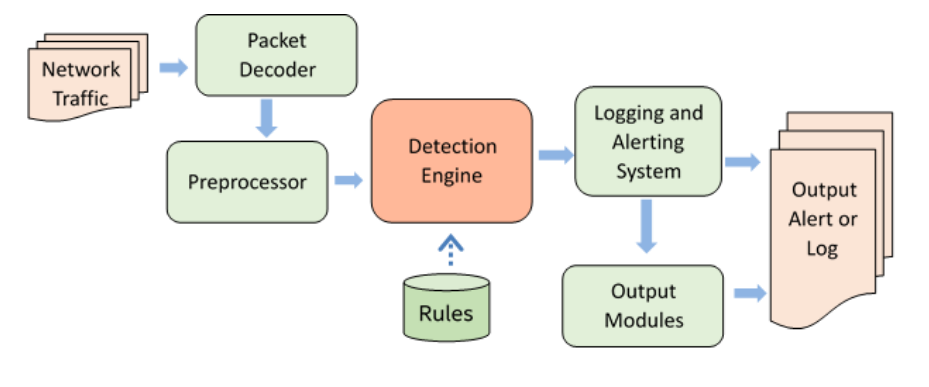
\includegraphics[width=0.7\textwidth]{Figuras/nids-funcionamento.png}


    \end{figure}

\end{frame}


\begin{frame}{NIDS: A Limitação da Criptografia e Modos de Sensor}
    \begin{itemize}
        \item \textbf{A Grande Limitação - Criptografia:}
              \begin{itemize}
                  \item Com o uso crescente de criptografia (ex: TLS/SSL), os NIDS \textbf{perderam o acesso ao conteúdo (payload)} significativo do tráfego.
                  \item Isso \textbf{prejudica (hindering)} sua capacidade de funcionar bem (ex: não podem ver comandos maliciosos dentro de uma sessão HTTPS).
                  \item \textbf{Conclusão:} NIDS são importantes, mas só podem formar \textbf{parte} da solução (Defesa em Profundidade).
              \end{itemize}

        \item \textbf{Tipos de Sensores de Rede (Modos):}

        \item \textbf{1. Sensor Inline }
              \begin{itemize}
                  \item Inserido em um segmento de rede; o tráfego \textbf{deve passar através} do sensor.
                  \item (Pode ser combinado com um firewall ou switch).
                  \item \textbf{Vantagem (IPS):} Permite \textbf{bloquear} um ataque quando detectado (atuando como IDS e \textbf{IPS} - Intrusion Prevention System).
              \end{itemize}

        \item \textbf{2. Sensor Passivo }
              \begin{itemize}
                  \item (Mais comum).
                  \item Monitora uma \textbf{cópia} do tráfego de rede; o tráfego real \textit{não} passa pelo dispositivo.
                  \item \textbf{Vantagem:} Mais eficiente, pois não adiciona um passo de manuseio extra (não contribui para o atraso/delay dos pacotes).
              \end{itemize}
    \end{itemize}
\end{frame}

\begin{frame}{NIDS: Configuração Passiva e Sensores Wireless (WIDS)}
    \begin{itemize}
        \item \textbf{Configuração Típica}
              \begin{itemize}
                  \item O sensor se conecta ao meio (ex: cabo de fibra óptica) através de um \textbf{"tap"} (derivação física).
                  \item O "tap" fornece ao sensor uma \textbf{cópia} de todo o tráfego da rede.
                  \item \textbf{Uso de Placas de Rede:}
                        \begin{itemize}
                            \item \textbf{NIC 1 (Coleta):} Conectada ao "tap". Geralmente \textbf{não possui um endereço IP}. Apenas coleta todo o tráfego (modo promíscuo).
                            \item \textbf{NIC 2 (Gerenciamento):} Conectada à rede \textbf{com um endereço IP}. Permite ao sensor se comunicar com o servidor de gerenciamento NIDS.
                        \end{itemize}
              \end{itemize}

        \item \textbf{Distinção: Sensores Wireless}
              \begin{itemize}
                  \item Pode ser \textit{inline} (incorporado em um Access Point - AP) ou \textit{passivo} (monitorando o tráfego "pelo ar").
                  \item \textbf{Função:} Apenas sensores wireless podem analisar o tráfego de \textbf{protocolo wireless} e detectar ataques específicos (ex: DoS wireless, sequestro de sessão, AP falso).
                  \item \textbf{WIDS (Wireless IDS):} Um NIDS focado exclusivamente em redes sem fio.
              \end{itemize}
    \end{itemize}
\end{frame}

\begin{frame}{Honeypots: Definição e Propósito}
    \begin{itemize}
        \item Honeypots (Potes de Mel) são \textbf{sistemas-isca (decoy systems)}.
        \item São projetados para \textbf{atrair (lure)} um atacante potencial para \textbf{longe} dos sistemas críticos.

        \item \textbf{Três Objetivos Principais:}
              \begin{itemize}
                  \item \textbf{1. Desviar (Divert):} Desviar um atacante de acessar sistemas críticos.
                  \item \textbf{2. Coletar Informações:} Coletar dados sobre a atividade do atacante (técnicas, ferramentas).
                  \item \textbf{3. Ganhar Tempo (Encourage):} Encorajar o atacante a ficar no sistema tempo suficiente para que os administradores possam responder.
              \end{itemize}

        \item \textbf{A Lógica Fundamental:}
              \begin{itemize}
                  \item O honeypot é preenchido com \textbf{informações fabricadas} (que parecem valiosas, mas um usuário legítimo nunca acessaria).
                  \item \textbf{Qualquer acesso} ao honeypot é, por definição, \textbf{suspeito}.
                  \item O sistema é instrumentado com monitores e loggers sensíveis.
                  \item Como o ataque "parece" ser bem-sucedido, os admins podem rastrear o atacante sem expor sistemas produtivos.
              \end{itemize}
    \end{itemize}
\end{frame}

\begin{frame}{Honeypots: Tipos de Interação (Low vs. High)}
    \begin{itemize}
        \item \textbf{Valor do Honeypot:} É um recurso sem valor de produção. Não há razão legítima para interação.
              \begin{itemize}
                  \item Qualquer comunicação \textit{de entrada} (inbound) é (provavelmente) uma sonda, scan ou ataque.
                  \item Se um honeypot inicia comunicação \textit{de saída} (outbound), ele (provavelmente) foi comprometido.
              \end{itemize}

        \item \textbf{Classificação (Nível de Interação):}

        \item \textbf{1. Low Interaction Honeypot (Baixa Interação)}
              \begin{itemize}
                  \item Um pacote de software que \textbf{EMULA} serviços ou sistemas (ex: finge ser um servidor FTP).
                  \item Fornece uma interação inicial realista, mas \textbf{não executa} a versão completa dos serviços.
              \end{itemize}

        \item \textbf{2. High Interaction Honeypot (Alta Interação)}
              \begin{itemize}
                  \item É um \textbf{sistema real}: S.O. completo, serviços e aplicações reais.
                  \item O sistema é instrumentado (monitorado) e colocado onde os atacantes podem acessá-lo.
              \end{itemize}
    \end{itemize}
\end{frame}

\begin{frame}{Trade-offs (High vs. Low) e Honeynets}
    \begin{itemize}
        \item \textbf{High Interaction (Vantagem):}
              \begin{itemize}
                  \item Um alvo \textbf{muito mais realista}.
                  \item Pode "ocupar" (prender) um atacante por um período extenso.
              \end{itemize}

        \item \textbf{High Interaction (Desvantagens / Riscos):}
              \begin{itemize}
                  \item Requer \textbf{significativamente mais recursos} (é um S.O. real).
                  \item \textbf{RISCO:} Se for comprometido, pode ser usado pelo atacante para iniciar ataques contra \textbf{outros sistemas} (na Internet).
                  \item Isso pode resultar em problemas \textbf{legais} ou de \textbf{reputação} indesejados para a organização.
              \end{itemize}

        \item \textbf{Low Interaction (Vantagem):}
              \begin{itemize}
                  \item Suficiente para detectar estágios iniciais do ataque (scan, probe) e alertar (como componente de um IDS distribuído).
              \end{itemize}

        \item \textbf{Honeynet (Rede Honeypot):}
              \begin{itemize}
                  \item Esforços recentes ("The Honeynet Project") focam em construir \textbf{redes inteiras} de honeypots que emulam uma empresa (com tráfego simulado).
              \end{itemize}
    \end{itemize}
\end{frame}

\begin{frame}{Implantação (Deployment) de Honeypots}
    \begin{itemize}
        \item A localização depende dos objetivos (tipo de info a coletar) e do nível de risco tolerado.
    \end{itemize}



    \begin{itemize}
        \item \textbf{1. Externo} (Internet, antes do firewall)
        \item \textbf{2. DMZ} (Rede de Serviços, entre firewalls)
        \item \textbf{3. Interno} (Rede Corporativa, após o firewall)
    \end{itemize}
\end{frame}

\begin{frame}{Implantação: Posição 1 (Externa)}
    \begin{itemize}
        \item \textbf{Localização:} Na Internet, \textbf{antes} do firewall externo.

        \item \textbf{Vantagens:}
              \begin{itemize}
                  \item Útil para rastrear tentativas de conexão a \textbf{IPs não utilizados} (scans).
                  \item \textbf{Não aumenta o risco} para a rede interna (o perigo de um sistema comprometido *atrás* do firewall é evitado).
                  \item \textbf{Reduz "ruído":} Atrai muitos ataques, reduzindo os alertas no firewall e nos sensores IDS internos (facilitando o gerenciamento).
              \end{itemize}

        \item \textbf{Desvantagem:}
              \begin{itemize}
                  \item Pouca ou nenhuma capacidade de capturar \textbf{atacantes internos}.
              \end{itemize}
    \end{itemize}
\end{frame}

\begin{frame}{Implantação: Posição 2 (DMZ)}
    \begin{itemize}
        \item \textbf{Localização:} Na rede de serviços (Web, Mail), ou seja, \textbf{dentro da DMZ} (entre o firewall externo e o interno).

        \item \textbf{Vantagem (Implícita):}
              \begin{itemize}
                  \item Monitora ataques direcionados aos serviços públicos (Web, Mail, DNS).
              \end{itemize}

        \item \textbf{Desvantagens (Trade-off):}
              \begin{itemize}
                  \item \textbf{Risco de Contaminação:} O admin deve garantir que os \textit{outros sistemas} (legítimos) na DMZ estejam seguros contra o honeypot (caso ele seja comprometido).
                  \item \textbf{Conflito com Firewall:} O firewall (externo) tipicamente \textbf{bloqueia} tráfego desnecessário para a DMZ (ex: permite só porta 80, 443).
                  \item \textbf{Dilema:} O admin deve (1) \textbf{abrir o firewall} (aumentando o risco) ou (2) \textbf{limitar a eficácia} do honeypot (que não verá os ataques bloqueados).
              \end{itemize}
    \end{itemize}
\end{frame}

\begin{frame}{Implantação: Posição 3 (Interna) e "Honeyfiles"}
    \begin{itemize}
        \item \textbf{Localização:} Na rede \textbf{totalmente interna}.

        \item \textbf{Vantagens:}
              \begin{itemize}
                  \item Vantagem mais importante: Pode capturar \textbf{ataques internos}.
                  \item Pode detectar um firewall \textbf{mal configurado} (que encaminha tráfego indevido da Internet para a rede interna).
              \end{itemize}

        \item \textbf{Desvantagens (Sérias):}
              \begin{itemize}
                  \item \textbf{Risco Alto:} Se o honeypot for comprometido, ele pode atacar \textbf{outros sistemas internos}.
                  \item (O firewall não bloquearia o tráfego do atacante para o honeypot, pois ele é visto como tráfego "permitido" para o honeypot).
                  \item (Similar à DMZ, o firewall interno precisa de regras de exceção).
              \end{itemize}
              \hrule
        \item \textbf{Tecnologia Relacionada: Honeyfiles}
              \begin{itemize}
                  \item Emulam \textbf{documentos} legítimos (com nomes realistas, ex: "Salarios\_Diretoria.xlsx").
                  \item Atuam como "isca" (bait) para intrusos.
                  \item \textbf{Qualquer acesso} a esses arquivos (que não deveriam ser acessados por usuários legítimos) é considerado \textbf{suspeito}.
              \end{itemize}
    \end{itemize}
\end{frame}



\begin{frame}[fragile]{Regra SNORT}
    \small
    \textbf{Regra Snort:}
    \begin{verbatim}
alert tcp $HOME_NET any -> $EXTERNAL_NET ![7680,1521] 
(msg:"ET P2P BitTorrent peer sync"; 
 flow:established,to_server; 
 content:"|00 00 00 0d 06 00|"; depth:6; 
 threshold: type limit, track by_dst, seconds 300, count 1; 
 reference:url,bitconjurer.org/BitTorrent/protocol.html; 
 classtype:policy-violation; sid:2000334; rev:14; 
 metadata:created_at 2010_07_30, confidence Medium, 
 signature_severity Informational, updated_at 2025_06_30;)
\end{verbatim}
\end{frame}



\begin{frame}{Cabeçalho da Regra}
    \small
    \texttt{alert tcp \$HOME\_NET any -> \$EXTERNAL\_NET ![7680,1521]}

    \begin{itemize}
        \item \textbf{alert}: gera um alerta quando a condição é atendida.
        \item \textbf{tcp}: apenas tráfego TCP.
        \item \textbf{\$HOME\_NET any}: origem na rede interna, qualquer porta.
        \item \textbf{\$EXTERNAL\_NET ![7680,1521]}: destino na rede externa, exceto portas 7680 e 1521.
    \end{itemize}
\end{frame}

\begin{frame}{Opções da Regra (1/2)}
    \small
    \texttt{msg:"ET P2P BitTorrent peer sync"; \\
        flow:established,to\_server; \\
        content:"|00 00 00 0d 06 00|"; depth:6;}

    \begin{itemize}
        \item \textbf{msg:} Mensagem exibida nos logs.
        \item \textbf{flow:established,to\_server:} Só considera conexões TCP já estabelecidas, indo para o servidor.
        \item \textbf{content:} Procura a sequência de bytes \texttt{00 00 00 0d 06 00}.
        \item \textbf{depth:6:} Pesquisa apenas nos primeiros 6 bytes do payload.
    \end{itemize}
\end{frame}

\begin{frame}{Opções da Regra (2/2)}
    \small
    \texttt{threshold: type limit, track by\_dst, seconds 300, count 1; \\
        reference:url,bitconjurer.org/BitTorrent/protocol.html; \\
        classtype:policy-violation; sid:2000334; rev:14;}

    \begin{itemize}
        \item \textbf{threshold:} Evita múltiplos alertas — 1 alerta por destino a cada 300s.
        \item \textbf{reference:} Link para a documentação do protocolo BitTorrent.
        \item \textbf{classtype:} Categoria: violação de política.
        \item \textbf{sid:} Identificador único (2000334).
        \item \textbf{rev:} Revisão nº 14.
    \end{itemize}
\end{frame}
%\title{Aula 16 - Vulnerabilidade de Software}

\author{Prof. Gabriel Rodrigues Caldas de Aquino}

\institute
{
    Instituto de Computação \\
    Universidade Federal do Rio de Janeiro\\
    gabrielaquino@ic.ufrj.br% Your institution for the title page
}
\date{Compilado em: \\ \today} % Date, can be changed to a custom date

%----------------------------------------------------------------------------------------
%    PRESENTATION SLIDE
%----------------------------------------------------------------------------------------



\begin{frame}
    % Print the title page as the first slide
    \titlepage
\end{frame}


\begin{frame}{Segurança de Software e Programação Defensiva}
    \begin{itemize}
        \item \textbf{A Raiz do Problema:}
              \begin{itemize}
                  \item Muitas vulnerabilidades de segurança resultam de \textbf{práticas de programação ruins}.
                  \item A conscientização sobre essas falhas é um passo inicial crítico para escrever código de programa mais seguro.
                  \item A lista dos 10 Principais Riscos de Segurança em Aplicações Web da OWASP inclui cinco falhas diretamente relacionadas a código de software inseguro.

                  \item \textbf{Estas falhas incluem:}
                        \begin{itemize}
                            \item Entrada de dados não validada.
                            \item Cross-site scripting (XSS).
                            \item Estouro de buffer.
                            \item Falhas de injeção.
                            \item Tratamento inadequado de erros.
                        \end{itemize}
              \end{itemize}
    \end{itemize}
\end{frame}

\begin{frame}{As Falhas Mais Perigosas (CWE/SANS Top 25)}
    \begin{itemize}
        \item A lista \textbf{CWE/SANS Top 25 Most Dangerous Software Errors} detalha o consenso sobre práticas que causam a maioria dos ciberataques.

        \item \textbf{As falhas são agrupadas em 3 categorias:}
              \begin{itemize}
                  \item \textbf{1. Interação Insegura entre Componentes.}
                  \item \textbf{2. Gerenciamento de Recursos Arriscado.}
                  \item \textbf{3. Defesas Porosas.}
              \end{itemize}
    \end{itemize}
\end{frame}

\begin{frame}{Categoria de Erro de Software: Interação Insegura entre Componentes}
    \begin{itemize}
        \item Neutralização Imprópria de Elementos Especiais usados em um Comando SQL (``Injeção de SQL'')
        \item Neutralização Imprópria de Elementos Especiais usados em um Comando do SO (``Injeção de Comando do SO'')
        \item Neutralização Imprópria de Entrada Durante a Geração de Página Web (``Cross-site Scripting'')
        \item Upload Irrestrito de Arquivo com Tipo Perigoso
        \item Falsificação de Solicitação entre Sites (CSRF)
        \item Redirecionamento de URL para Site Não Confiável (``Redirecionamento Aberto'')
    \end{itemize}
\end{frame}

\begin{frame}{Categoria de Erro de Software: Gerenciamento de Recursos Arriscado}
    \begin{itemize}
        \item Cópia de Buffer sem Verificar o Tamanho da Entrada (``Estouro de Buffer Clássico'')
        \item Limitação Imprópria de um Nome de Caminho para um Diretório Restrito (``Path Traversal'')
        \item Download de Código Sem Verificação de Integridade
        \item Inclusão de Funcionalidade de Esfera de Controle Não Confiável
        \item Uso de Função Potencialmente Perigosa
        \item Cálculo Incorreto do Tamanho do Buffer
        \item String de Formatação Não Controlada
        \item Estouro de Inteiro ou \textit{Wraparound}
    \end{itemize}
\end{frame}

\end{document}